\documentclass[a4paper,12pt]{extarticle}
\usepackage[utf8]{inputenc}
\usepackage{graphicx}
\usepackage{natbib}
\usepackage{amsmath}
\usepackage{caption}
\usepackage{subcaption}
\usepackage{geometry}
    \geometry{a4paper}
\bibliographystyle{plainnat}


\title{Discovering Focused Microgenre Communities}

\begin{document}
\maketitle
\subsubsection*{Abstract} 
Recent work in the sociology of taste has begun to grapple directly with the relational properties of traditional survey-based data using techniques inspired by network analysis. Despite the generally salutary results from this endeavor, critics rightly question the face and ecological validity of the vague macrogenre labels included in standard arts participation surveys (e.g., Classical, Rock, Rap). To deal with this issue, in this paper, I propose a link-clustering approach for discovering focused microgenres from standard survey-based information on cultural tastes, one that exploits the underlying relational patterns realized by the indirect connectivity structure of genres (via persons) in a two-mode network. The link-clustering approach partially answers two of the challenges of macro-genre critics: The fact that actual genres are overlapping and not crisply bounded and the fact that there is hidden heterogeneity within the broad labels we usually focus on. To demonstrate the validity of the approach, I contrast the application of the usual techniques to the same data, conceived in the usual ``macro" way, and after discovering hidden microgenres. The results reveal an intuitive partition of traditional macrogenres into focused microgenres, capable of separating audiences along relevant sociodemographic markers, such as education, ethnoracial identity, subjective class identification, and age/generation. 
\newpage

\section{Persons and Cultural Choices}
Recent work in the sociology of taste has blurred the distinction, foundational for much early work, between ``relational'' network data (codifying the relationships between people) and survey data (codifying the relationship between people and ``variables''). The basic idea is that all data, whether collected purposefully as ``network'' data or collected as part of a social survey, is \textit{relational} data. The main difference is the types of entities that are related \citep{borgatti_everett97}. That is, any data source that can be stored in matrix form has ``modes'' (how many types of entities are related) and ``ways'' (the number of entities linked by a relation, usually two at a time). The standard network data set is ``one mode'' (we usually look at one type of entity at a time, like people, organizations, schools, countries, and the like) and two ``ways'' (people-by-people or organization-by-organization pairs). In the same way, the usual person-by-variables survey data has two modes and two ways. The relations are not people-by-people but people-by-variables. People are connected to the survey items they answer by relations of affinity, disagreement, choice, or even negatively (by not answering). Following, \citet{breiger74}, it is possible to recover person-by-person (one mode, two ways) matrices from the usual person-by-variables data matrices. People can be connected to others if they share the same values, opinions, tastes, practices, or demographics recorded as variables in the columns of the matrix. 

When transplanted to the sociology of taste, for which survey data has been the workhorse source of insights and empirical generalizations \citep{peterson_kern96, bryson96, vaneijck01,savage_gayo11}, this blurring of the boundaries between the two main sources of relational data in the social sciences can be revelatory. This goes beyond the fact, to be exploited below, that once we treat survey data as network data, then the entire methodological panoply developed by social network analysts (and increasingly ``network scientists'' working across many disciplines) for the last fifty or so years becomes part of the analytic toolbox. In addition to this, the entire \textit{conceptual} arsenal of social network theory \citep{borgatti11} also becomes available. As \citet[244]{borgatti_everett97} note, once we convert ``2-mode data sets into 1-mode matrices{\dots}we can then apply the techniques (if not the theories) of network analysis.''

Accordingly, a spate of recent work has begun the job of theoretical translation, enriching the first-generation of work in the sociology of taste with network-flavored concepts. Accordingly, \citet{pachucki2010cultural} extend Ronald Burt's theory of structural holes for understanding how people can bridge gaps not just in one-mode person-to-person networks but in two-mode person-to-culture networks. Following this lead, \citet{lizardo14} provides a metric based on Burt's conception of network efficiency that is meant to characterize the slippery concept of ``omnivorousness" concerning genres and cultural forms that people engage in. This approach goes beyond just summing or counting people's cultural engagements to consider the audience overlap between the genres themselves. Thus, the true omnivore is a person who consumes genres with low audience overlap. Other work in this same vein extends ideas related to positional equivalence in networks \citet{breiger1976social} to uncover ``blocks'' of respondents that tend to dislike the same set of genres that others like \citep{okada2017structure}. A similar approach, based on ideas of positional equivalence in networks, can be extended beyond the study of beliefs and social attitudes more generally to identify respondents who share cultural schemas \citep{goldberg2011mapping}. \citet{lizardo18} adapts techniques first developed for the study of economic complexity in two-mode networks of geographic sites and products/technologies for the characterization of genres (e.g., popular versus niche) and audience (e.g., omnivore versus ``univore'') characteristics in survey data on cultural tastes. 

\section{The Problem of Genre in the Sociology of Taste}
In this paper, I continue to ride this wave of adapting network approaches to survey data on cultural tastes to tackle a fundamental problem (both substantive and measurement-wise) in the sociology of taste, namely, the problem of \textit{genre}. In a foundational paper, \citet{dimaggio1987classification} provided a prescient conceptualization of the core constructs of the sociology of taste in a way that exploited the network imagery that has become a routine reality of late. In the paper, \citet[244]{dimaggio1987classification} asked us to

\begin{quote}
   {\dots}imagine a matrix defined by persons on the vertical axis and artworks on the horizontal axis, with{\dots}signifying relationships (knowledge about, like for, dislike of) between person and artworks, genres consist of those sets of works which bear similar relations to the same set of persons. The logic behind this imagery will be familiar to students of network analysis as one of ``structural equivalence.''
\end{quote}

Thus, for DiMaggio, genres are dual entities precisely in Breiger's sense defined above. Genre categories are composed of the audiences that engage them (are subsets of the larger set of people). People, on the other hand, are related to one another (e.g., via relations of similarity, opposition, or non-overlap) by the genres they choose, and genres related to one another via overlaps (intersections) in the sets of people who choose them \citet{lizardo18}. 

This conceptualization, like a lot of network theorizing, is elegant but gets messy in the application. As \citet[149]{lena2015relational} has noted, ``[n]o ordering principle is as fundamental to culture as genre'' yet, none is also as vexed. One issue Lena raises is that sociologists have relational intuitions about genres but tend to default to musicological definitions for convenience's sake. Thus, when it comes to considering which genres to include in a survey on cultural tastes, the tendency is simply to pick off the shelf from the menu of genre categories. The problem with these folk genre classifications is that they tend to miss the fuzzy, overlapping ways that real-world genres are organized. This leads us to treat what are, in fact, contested boundaries as if they were natural, crisp boundaries (e.g., assigning respondents who like ``Rap" to a different taste community than those who like ``Opera."). This is the problem of \textit{overlapping boundaries among genre categories}. 

The other issue has to do with the level of aggregation. For convenience’s sake, survey data must settle on a ``middle'' level of categorization so as not to tax respondents' patience (or knowledge). Thus, the standard ``lists'' of cultural genres, such as ``Pop Art,'' ``Romantic Comedy," or ``Blues.'' However, as recent work points out, people, venues, fandoms, scenes, subcultures, communities, organizations, critics, gatekeepers, and even states and other powerful institutions, make sociologically relevant distinctions within macro-genres categories \citep{hesmondhalgh2005subcultures, Holt2007, Van_Poecke2018}. Genres may also develop and accumulate subvariations as they ``travel'' across production, dissemination, and consumption sites in their historical trajectory \citep{Lena2012}. These ``micro-genres'' are embedded within larger macro-genres in complex ways that the standard survey approach misses. 

\section{What to do about the problem of genre}
One solution to the problem posed by vague macro-genre labels, suggested by \citet{vlegels2015music, vlegels2017music} concerning musical genres, is to ``change the mode'' and ``drop the label'' by asking respondents not just for their levels of engagement or liking of broad macro-genre labels but for performers within those labels. This work shows that once these ``micro-genre'' distinctions based on performers are made, some core empirical generalizations in the sociology of taste (e.g., highly educated people like classical music) are controverted or at least heavily qualified. This \textit{micro-genre heterogeneity} critique thus asserts that the standard genre labels studied by social scientist hide as much as they reveal because micro-genre communities can be internally diverse and even contain mutually opposed groups in the social space \citep{flemmen_etal18}. For people, the unit of selection and judgment is the {\em micro-genre}, not the broad genre classification, so it is unclear what to do (and how to interpret) the usual data collected by sociologists who study taste using surveys. 

But what happens when all the data we have (as it is with the long-standing surveys such as the Survey for Public Participation in the Arts or the General Social Survey) is at the macro-genre label? Both overlapping boundary and micro-genre heterogeneity critics of traditional genre labels would say to simply ignore these data and collect new data that does not rely on misleading macro-genre labels. Here I propose another solution: {\em Exploit the inherent relationality embedded in survey data responses} \citep{goldberg2011mapping, boutyline2017belief, lizardo18}. 

More specifically, my point will be that by exploiting the inherent relationality already contained in the usual survey data (when treated as two-mode network data), old data can reveal insights that pertain to the very features sociological critics of the macro-genre label concept say is missing. In particular, it is possible to use embedded sets of relations between people and genres to discover the very heterogeneous micro-genre communities critics say are hidden by the macro-genre label (thus my point is that these are hidden but not necessarily absent). This approach is thus ideal for making new use of old data. 	

\subsection{Precursors of the Proposed Approach}
The approach proposed here builds on the core ideas of ``duality'' and ``relationality'' that have  become foundational for formal approaches to measuring culture in the sociology of taste \citep{mutzel2020duality, mohr2015formal}. In this sense, I followed a path already trailed by others. For instance, Goldberg's \citeyearpar{goldberg2011mapping} {\em Relational Class Analysis} (RCA) ``classifies the people'' (in the terms developed below when reviewing standard data-analytic approaches in the sociology of taste) included a survey by partitioning a person-by-person matrix built from higher order similarities (sums of differences of differences) between each pair of person's corresponding response vector coding their stances (e.g., like, dislike, neutral) toward a set of cultural objects (e.g., genres, attitude items). Boutyline's 
\citeyearpar{boutyline2017improving} {\em Correlational Class Analysis} (CCA) also classifies the people but this time by using the absolute value of the correlation distance between response vectors to build the person-by-person similarity matrix. Boutyline and Vaisey's {\em Belief Network Analysis} (BNA) classifies the objects people connect to (in their case, beliefs, but could also be genres) by creating a weighted object network, where the weight of the tie between two objects (attitude toward government spending and attitude toward immigration) is given by the magnitude of their correlation coefficient in the survey. 

As we will see, I propose an approach thoroughly complementary to and synergistic with these previous efforts. More to the point, the relational identification of microgenres should be able to improve the applicability of techniques like RCA, CCA, and BNA (and related techniques), because, just like standard statistical approaches (like Factor Analysis, Principal Component Analysis, Latent Class Analysis and so forth), and even techniques (like Multiple Correspondence Analysis that are sometimes opposed to the traditional statistical ones, these newfangled relational techniques are also dragged down by the macrogenre curse. Thus, RCA and CCA are bound to compute relationality and correlation distances within people but have to rely on vague macrogenre labels. The resulting evaluation logics are thus interpreted using a macrogenre lens---e.g., ``Anything but Heavy Metal'' or ``Highbrow versus Lowbrow" \citep[e.g.,][]{goldberg2011mapping, willekens2022cultural}. But what if what one group means by "Heavy Metal" differs from what another group means by the same vague label? Are we sure that certain {\em all} types of classical music are ``opposed'' to or divergent from engagement with Country or Hip Hop? Some versions of Indie/Alt Rock are considered today as ``highbrow'' as Classical music (used to be) \citep{Van_Poecke2018}; or there may exist types of Country music that appeal to highly educated audiences and, thus, to people who might also listen to musicals? Overall, all quantitative techniques used by researchers in the sociology of taste must work with the (broad) genre categories included in the survey they are powerless to deal with these (reasonable) objections. 

Importantly, this implies that the clumping of vague macrogenre labels into even vaguer meta-macrogenres (discourses, styles, logics, schemas) like ``highbrow'' could be a spurious by-product of the vague labeling (as micro-genres critics have long suspected). This matters because such macrogenre clumping does much conceptual (and technical) work in our data reduction, data interpretation, and substantive theorizing efforts. The result is that it is likely that people are classified as following the same cultural logic of genre valuation and evaluation when they, in fact, follow distinct logics. In fact, a key implication of the approach to be described below is that regardless of the particular technique used, sociologists of taste are likely to underestimate population heterogeneity in the logics of classification and evaluation people use to navigate the cultural space \citep{lahire2008individual}. This heterogeneity has to be {\em revealed} before constructing belief or attitude networks, classifying people into schematic classes, embedding genres into a dimensional space, or putting people into latent classes.

\subsection{Data to be Used in the Study}
The empirical part of the study uses data on the musical tastes of American collected with Sara Skiles in the summer of 2012 \citep{lizardo_skiles15, lizardo_skiles16}. The survey was (partially) designed to replicate the General Social Survey (GSS) 1993 Culture Module. This is now a canonical data set providing the empirical basis for a variety of analyses (and reanalyses) in the sociology of taste \citep[e.g.,][]{bryson96, goldberg2011mapping, schultz2010strength, han2003unraveling, tampubolon2008revisiting, okada2017structure}.  The data were collected by an organization then called Survey Sample International (SSI), a private firm specializing in sampling, data collection, and analysis. SSI managed recruitment and participation invitation tasks to generate a panel of adults from which our working sample was drawn. Survey respondents were selected from the panel for participation based on age, gender, race, education, and geographic region to approximate a sample representative of the U.S. population ($n = 2,263$). Like GSS 1993, SSI 2012 included items assessing respondents’ likes and dislikes (as well as a middle category of ``mixed feelings'') for 20 categories of musical style: classical/ symphony and chamber, opera/operetta, jazz, Broadway musicals/show tunes, mood/easy listening, big band/swing, classic rock/oldies, country, bluegrass, folk, hymns/gospel, Latin/Spanish/salsa, rap/hip hop, blues/R\&B, reggae, top 40/pop music, contemporary rock, indie/alternative rock, dance/club/electronic, and hard rock/heavy metal. In addition to providing a taste judgment for each item, respondents were also asked if they regularly listened to each macro-genre. The following analyses are based on a data frame in which people are coded as engaging the macro-genre if they report both liking and listening to it. The two-mode network we will be working with is thus of dimensions and has $2263$ people and $20$ genres. This defines an affiliation matrix $A_{PG}$ of the same dimensions, with entries equal to 1 if person $P$ likes \textit{and} listens to macro-genre label $G$ and zero otherwise. 

\subsection{The Link Clustering Approach}
I propose that exploiting {\em relationality} hidden in the usual survey data collecting information on people and genres can help us make headway on the micro-genre critique outlined in the preceding. As noted at the outset, this requires that we stop looking at the usual survey data that forms the bulk of empirical material in the quantitative study of taste as ``survey data'' (e.g., data collected on the characteristics of individuals in the form of ``variables''). This is a presumption that is baked into traditional techniques (like Factor Analysis or Latent Class Analysis) that fit statistical models to such data. It is also embedded in ``relational'' techniques like Multiple Correspondence Analysis which, while not steeped in the preoccupations of standard statistical inference (although it could be), divert our attention to the indirect relations between macro-genres (or between people), usually conceptualized as distances in a social space. This kind of indirect relationality is fine and dandy but as already noted in the case of RCA, CCA, and BNA, all the relationality built into MCA is powerless, if what is fed {\em into} the process is the same old, limited, overextended macro-genre categories. 

I address the micro-genre issue using a technique for overlapping community detection called link clustering \citep{ahn_etal10}. The basic idea is simple and is illustrated in the toy example shown in Figure~\ref{fig:link-toy1}. Breaking with approaches that attempt to cluster people and genres by focusing on the people or the genres, we take the person-to-genre {\em link} as the unit of analysis and focus our classification energies on those. Classifying the links gives (by definition) a classification of the entities at the end of each link (people and genres) for free. Not only that, because most people choose multiple genres, and all genres ``choose'' multiple people, this classification guarantees that genres get assigned to multiple \textit{overlapping} clusters, at the same time splitting up the macro-genres into more relationally focused clumps. This allows us to make headway on both horns of the micro-genre critique---namely, overlapping categories and internal differentiation---at once.

\begin{figure}[ht!]
     \centering
     \begin{subfigure}[b]{0.6\textwidth}
        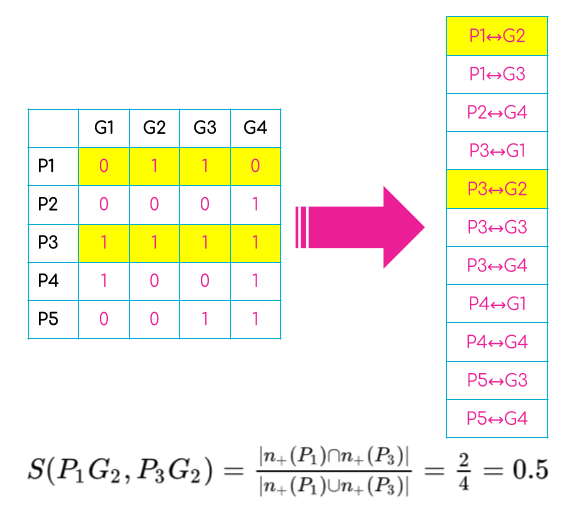
\includegraphics[width=1.0\textwidth]{Figs/Toy/link-clust-toy1.png}
        \caption{Two person-genre edges sharing the same genre.}
        \label{fig:link-toy1}
    \end{subfigure} 
     \begin{subfigure}[b]{0.3\textwidth}
        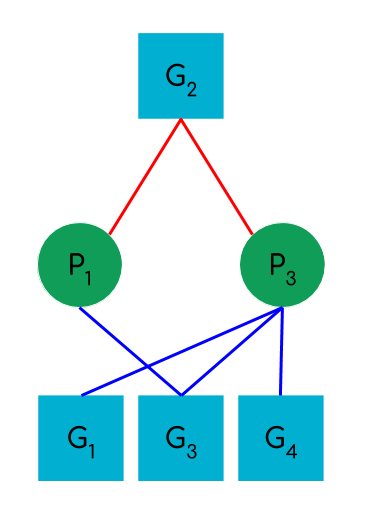
\includegraphics[width=1.0\textwidth]{Figs/Toy/link-clust-toy2.png}
        \caption{Similarity between person-genre edges depends on the other genres people are linked to.}
        \label{fig:link-toy2}
    \end{subfigure}
     \begin{subfigure}[b]{0.45\textwidth}
        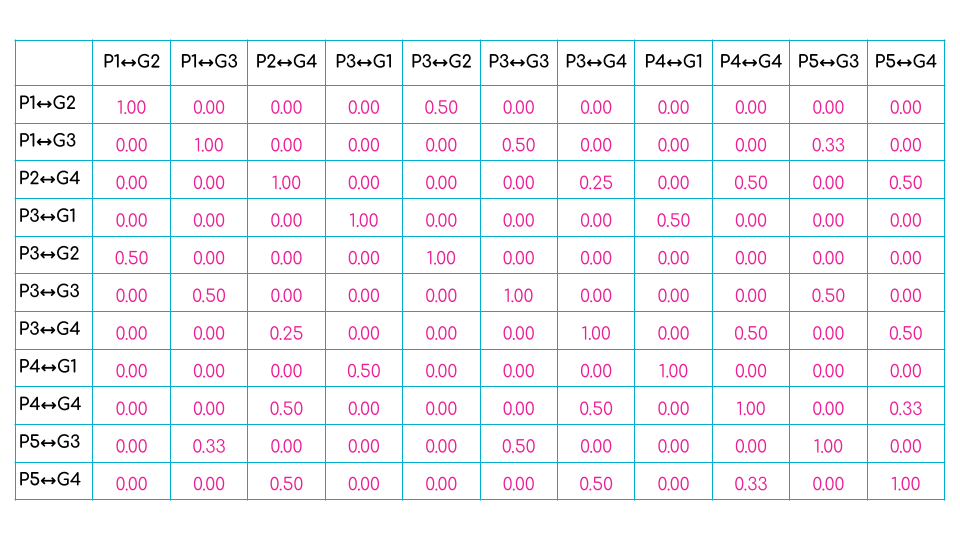
\includegraphics[width=1.0\textwidth]{Figs/Toy/link-clust-toy3.png}
        \caption{Edge similarity matrix from toy example.}
        \label{fig:link-toy3}
    \end{subfigure}
     \begin{subfigure}[b]{0.45\textwidth}
        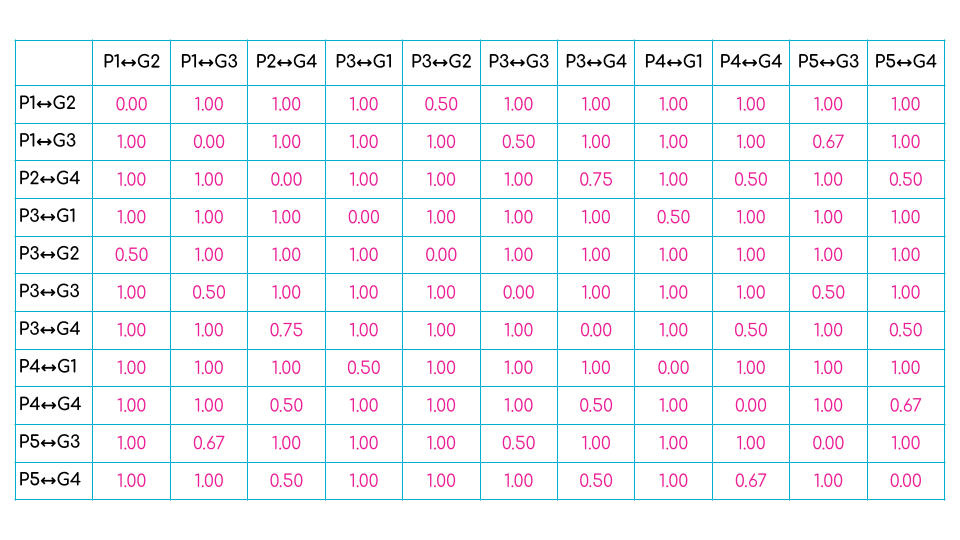
\includegraphics[width=1.0\textwidth]{Figs/Toy/link-clust-toy4.png}
        \caption{Edge distance matrix from toy example.}
        \label{fig:link-toy4}
    \end{subfigure}
     \begin{subfigure}[b]{0.6\textwidth}
        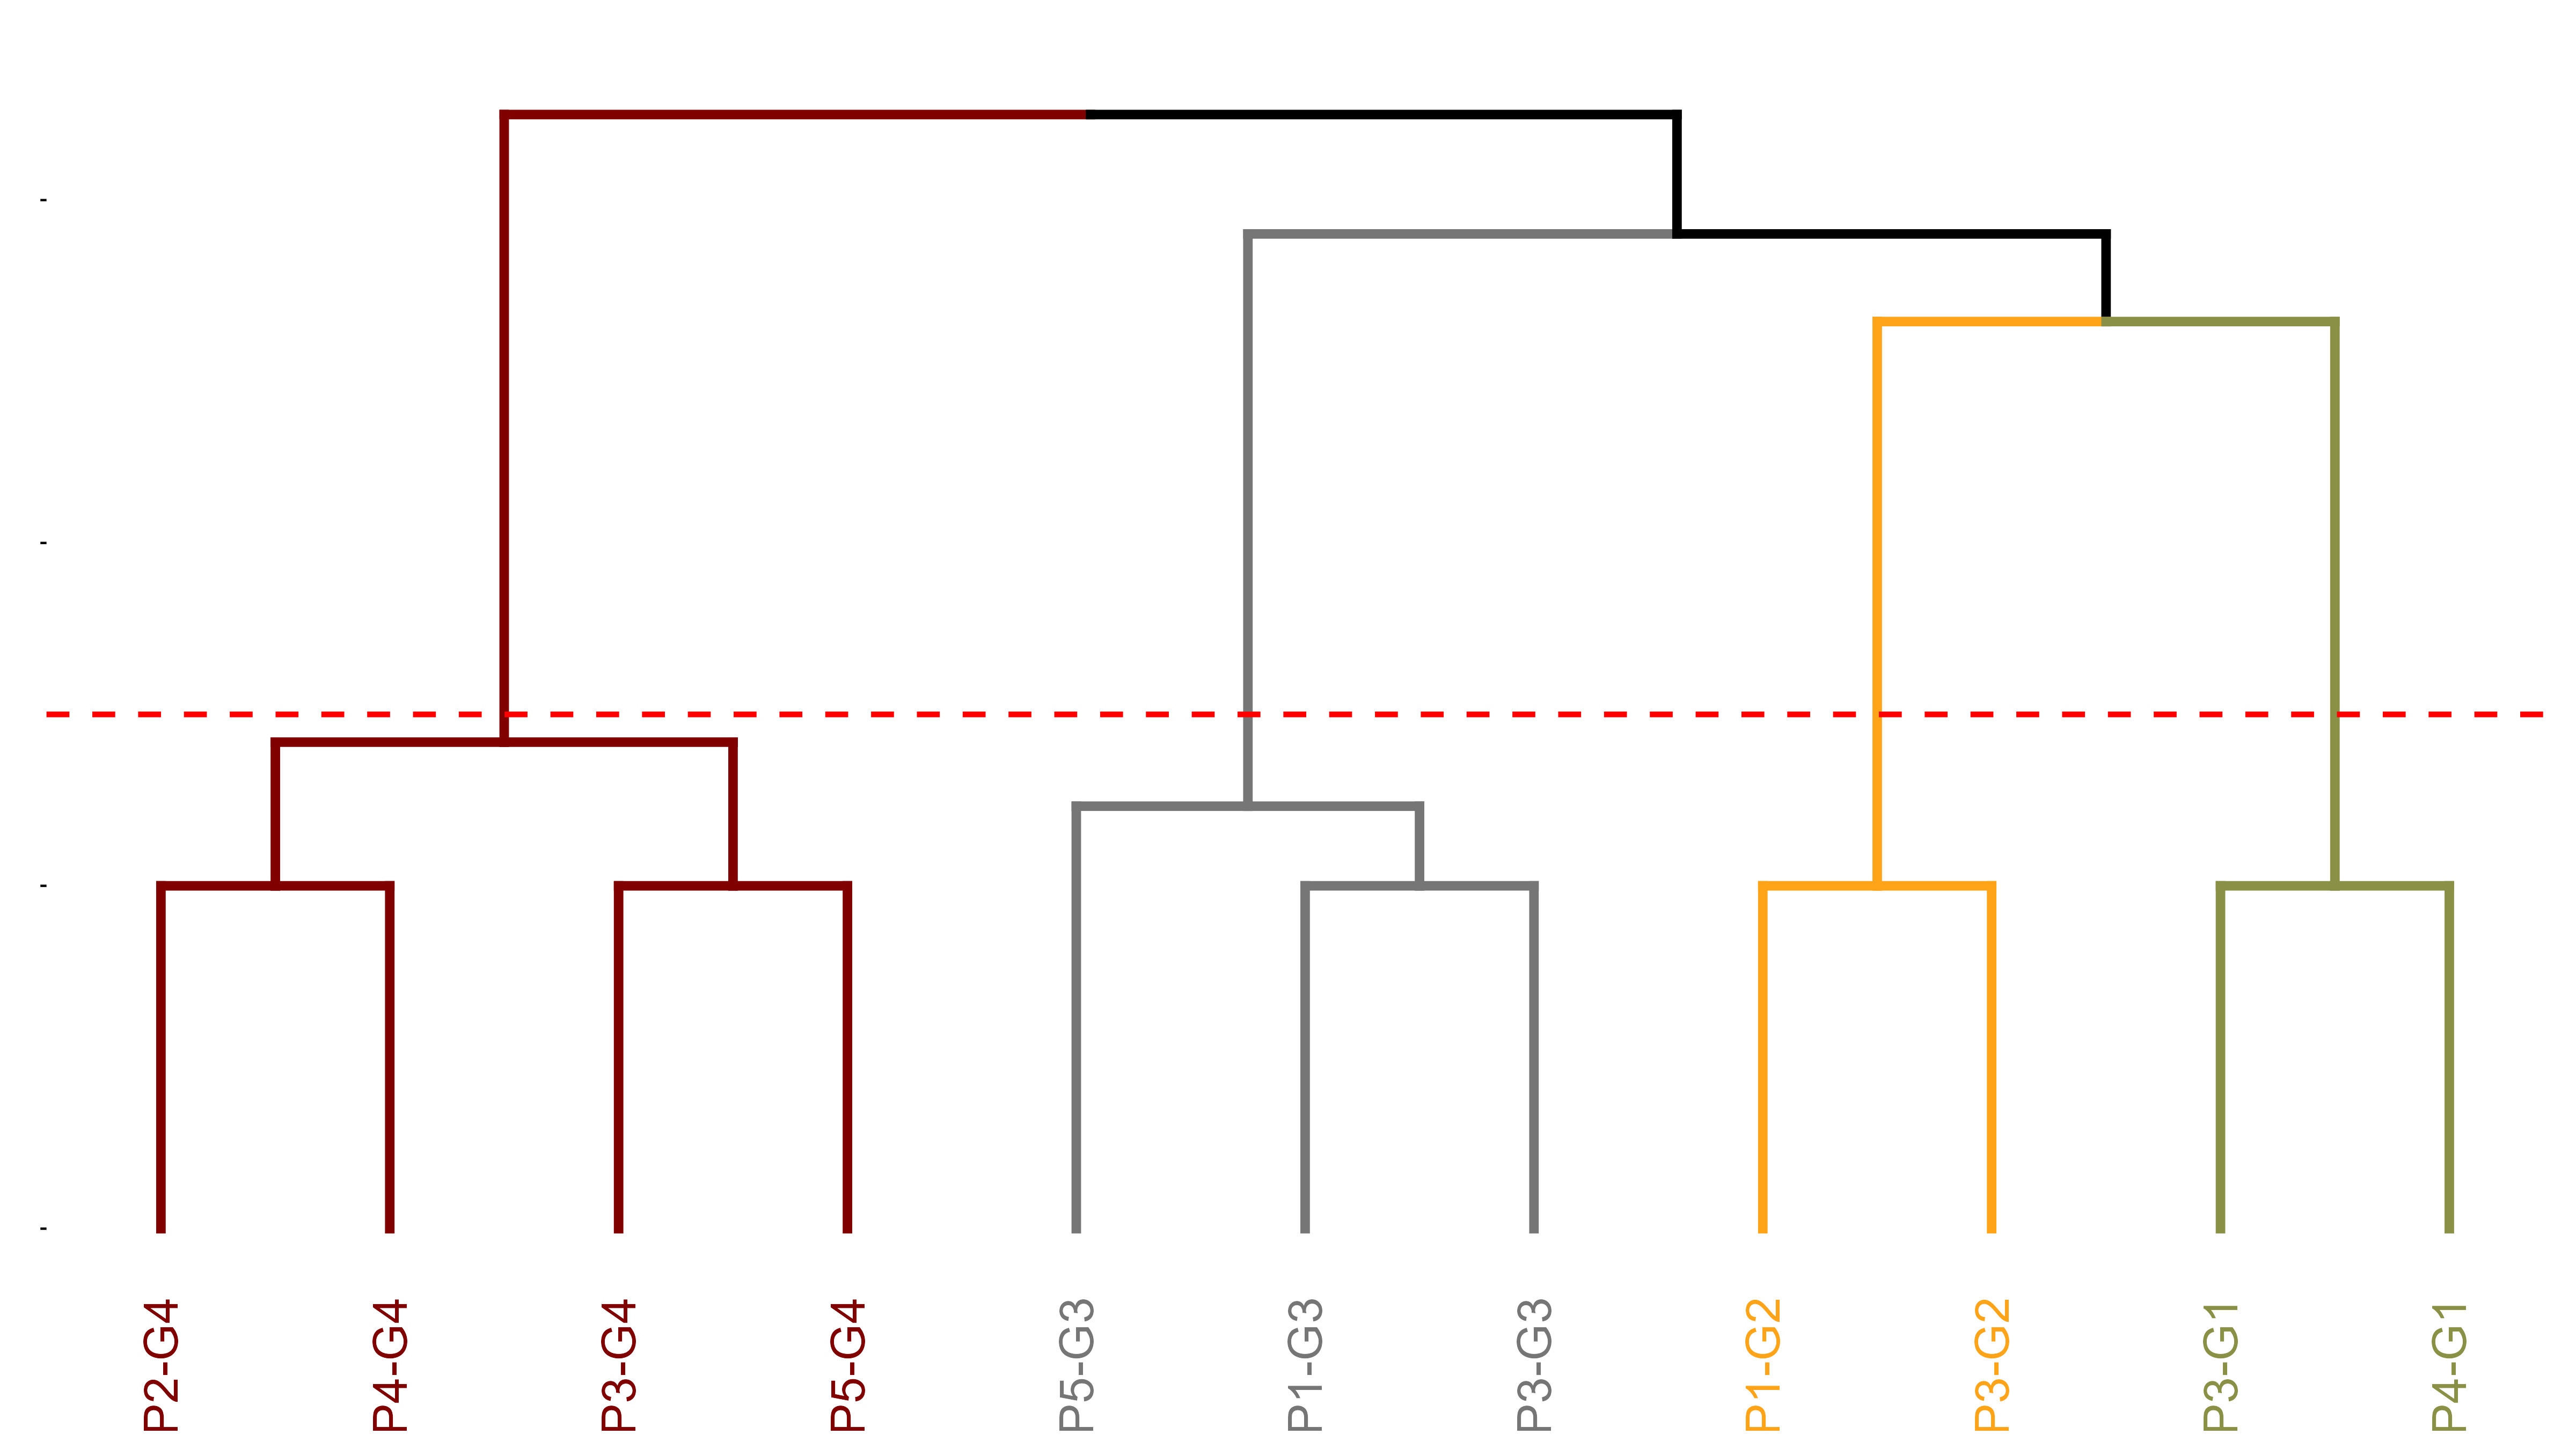
\includegraphics[width=1.0\textwidth]{Figs/Toy/link-clust-toy5.png}
        \caption{Dendrogram from Ward clustering of toy example edge distance matrix cut at four clusters.}
        \label{fig:link-toy5}
    \end{subfigure}
    \caption{Toy illustration of how the link clustering approach works.}
    \label{fig:link-toy}
 \end{figure}
 
How does this work? As Figure~\ref{fig:link-toy1} shows, once we string out the original two-mode person-by-network in our toy example into an edge list (now containing eleven person-genre edges), where the cases are the person to genre pairs that are marked by a ``1'' in the original matrix, it is possible to ask: ``How similar is one edge to another?'' We can answer that question as follows. The similarity of one person-to-genre edge to another, when both edges point to the same genre \citep{ahn_etal10}, should be proportional to the overlap between the ``cultural ego networks'' of the two people at the tail end of the edges. As \citet{lizardo14} defines it, for any respondent $i$, in a survey on cultural taste, the cultural ego network is simply the set of genres $\{G_1, G_2,\dots G_k\}$ chosen by the person. 

Going back to our running toy example, we are tasked with computing the similarities between $\frac{11 \times (11-1)}{2} = 55$ person to genre pairs. Suppose we wanted to calculate the similarity between the $P_1-G_2$ and $P_3-G_2$ person-to-genre edges in the two-mode network. In Figure~\ref{fig:link-toy1}, these two links are highlighted in yellow the ``strung out'' edgelist and are shown in red in the corresponding bipartite subgraph shown in Figure~\ref{fig:link-toy2}. The similarity ($S$) between the two links is then given by:

\begin{equation}
    S(P_1G_2, P_3G_2) = \frac{n_+(P_1) \cap n_+(P_3)}{n_+(P_1) \cup n_+(P_3)}
\end{equation}

Where $n_+(P_1)$ is the cultural ego network of Person 1 and $n_+(P_3)$ is the cultural ego network of Person 3. The formula says that the similarity between two person-to-genre links sharing a genre, in this case, the similarity between the $P_1-G_2$ edge and the $P_3-G_2$ edge, is given by the intersection of Person 1's and Person 3's cultural ego network divided by their union (also known as Jaccard's coefficient). When the cultural ego networks of two people are the same then $S=1$, when they are completely disjoint (share no genres, meaning the intersection is the empty set), then $S = 0$. All other cases of person-to-genre edges sharing the same genre return a number between zero and one ($0 > S < 1$).\footnote{Note that the only substantive similarities we care about are between person-to-genre edges that shared the same genre but have different people attached to them at the other end. All other person-to-genre edges, featuring people connected to different genres are set to zero.} In the toy example case, $P_1$ and $P_3$ consume two genres out of the four possible ones they could consume in common, resulting in an edge similarity score of $\frac{2}{4} = 0.50$. 

If we do that for all pairs of person-to-culture genres sharing one genre node in common, we end up with the two-way, one-mode (now the only mode is edges) $11 \times 11$ similarity matrix shown in Figure~\ref{fig:link-toy3}. Note two features of the similarity matrix. First, by definition two person-to-genre links that go from different genres to the same person are maximally similar (as the overlap is 1.0). This means that only links that go from different people to the same genre exhibit overlap variation, and this is driven (``reflectively'' \citep{lizardo18}) by the overlap between the neighborhoods of the other mode (people). Next, we transform the similarity matrix into a {\em dissimilarity} matrix by subtracting one from each entry (shown in  Figure~\ref{fig:link-toy4}). We then subject this matrix to hierarchical clustering using Ward's \citeyearpar{ward63} method. 

The resulting dendrogram from the cluster analysis is shown in Figure~\ref{fig:link-toy5}. Note that moving from the top down, the dendrogram splits person-to-genre links according to the macro-genre label. That is macro-genre information is preserved in the clustering, and can be recovered by splitting the dendrogram at a height where the number of clusters is equal to the original number of macro-genres (in this case, four as shown in Figure~\ref{fig:link-toy5}). Moving from the bottom up, the hierarchical clustering of the dissimilarity matrix yields {\em link communities} \citep{ahn_etal10}, in which both people nodes, but, most crucially, genres nodes are assigned to different clumps. In the limiting case (the bottom-most ``leafs'' of the dendrogram, each person-to-genre links are assigned to their cluster. The more interesting thing is that as we move up to a point below macro-genres clusters and above the leafs, we see a partition of {\em varieties} of macro-genres. For instance, macro-genre $G4$ is split into two focused micro-genre varieties. The first is attached to persons $P2$ and $P4$ and the second attached to persons $P3$ and $P5$ respectively. The idea then, is that the macro-genre nodes (e.g., ``Classical,'') assigned to different clumps represent micro-variations of the macro-genre label that differ primarily in a relational or structural way; different ``types'' of ``Classical'' are different because their audiences make distinct choices {\em with respect} to the other genres in the survey. 

\begin{figure}[ht!]
     \begin{subfigure}[b]{0.5\textwidth}
        \centering
        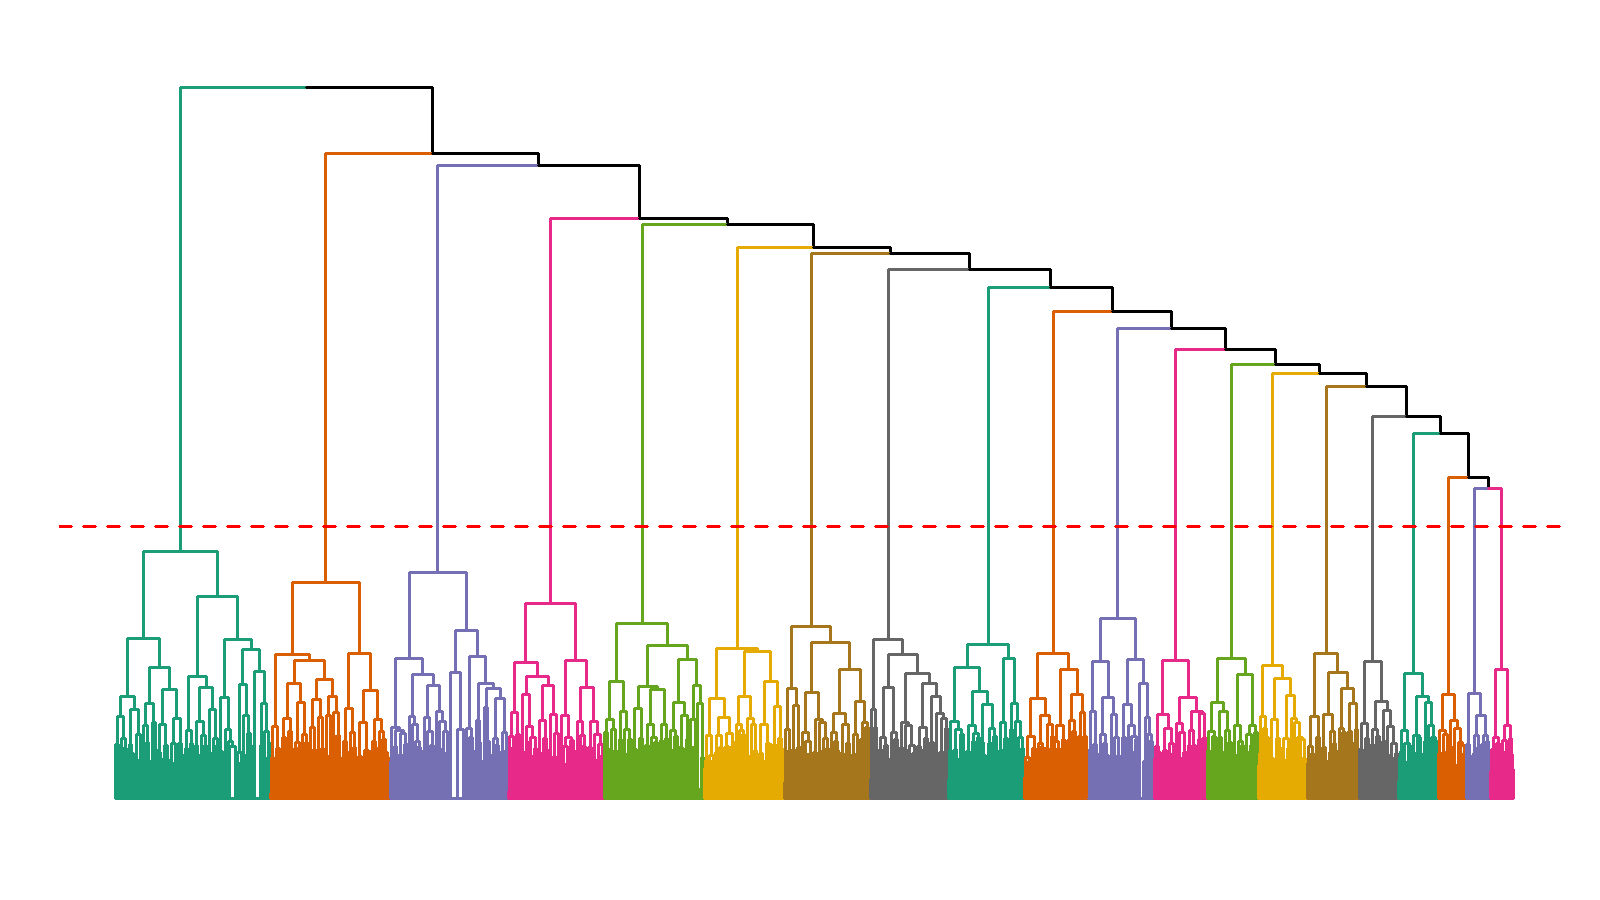
\includegraphics[width=1.0\textwidth]{Figs/Dend/all-branches-macro.png}
        \caption{c = 8, k = 20}
        \label{fig:dend-macro}
    \end{subfigure} 
     \begin{subfigure}[b]{0.5\textwidth}
        \centering
        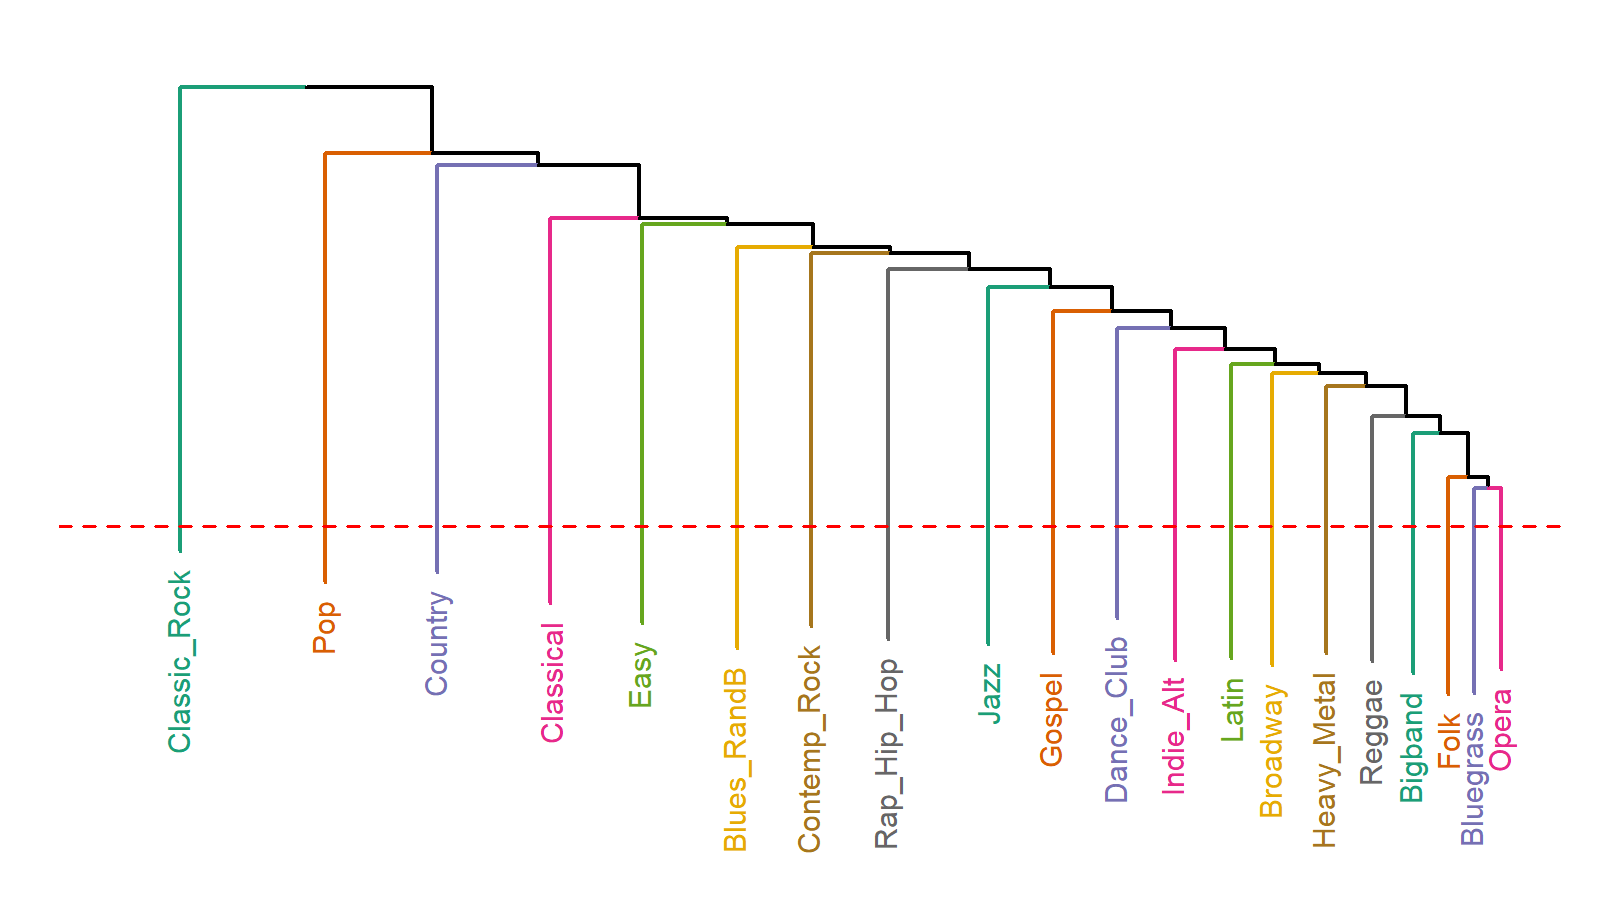
\includegraphics[width=1.0\textwidth]{Figs/Dend/all-branches-macro-labels.png}
        \caption{c = 8, k = 20}
        \label{fig:dend-macro-labels}
    \end{subfigure} 
     \begin{subfigure}[b]{0.5\textwidth}
        \centering
        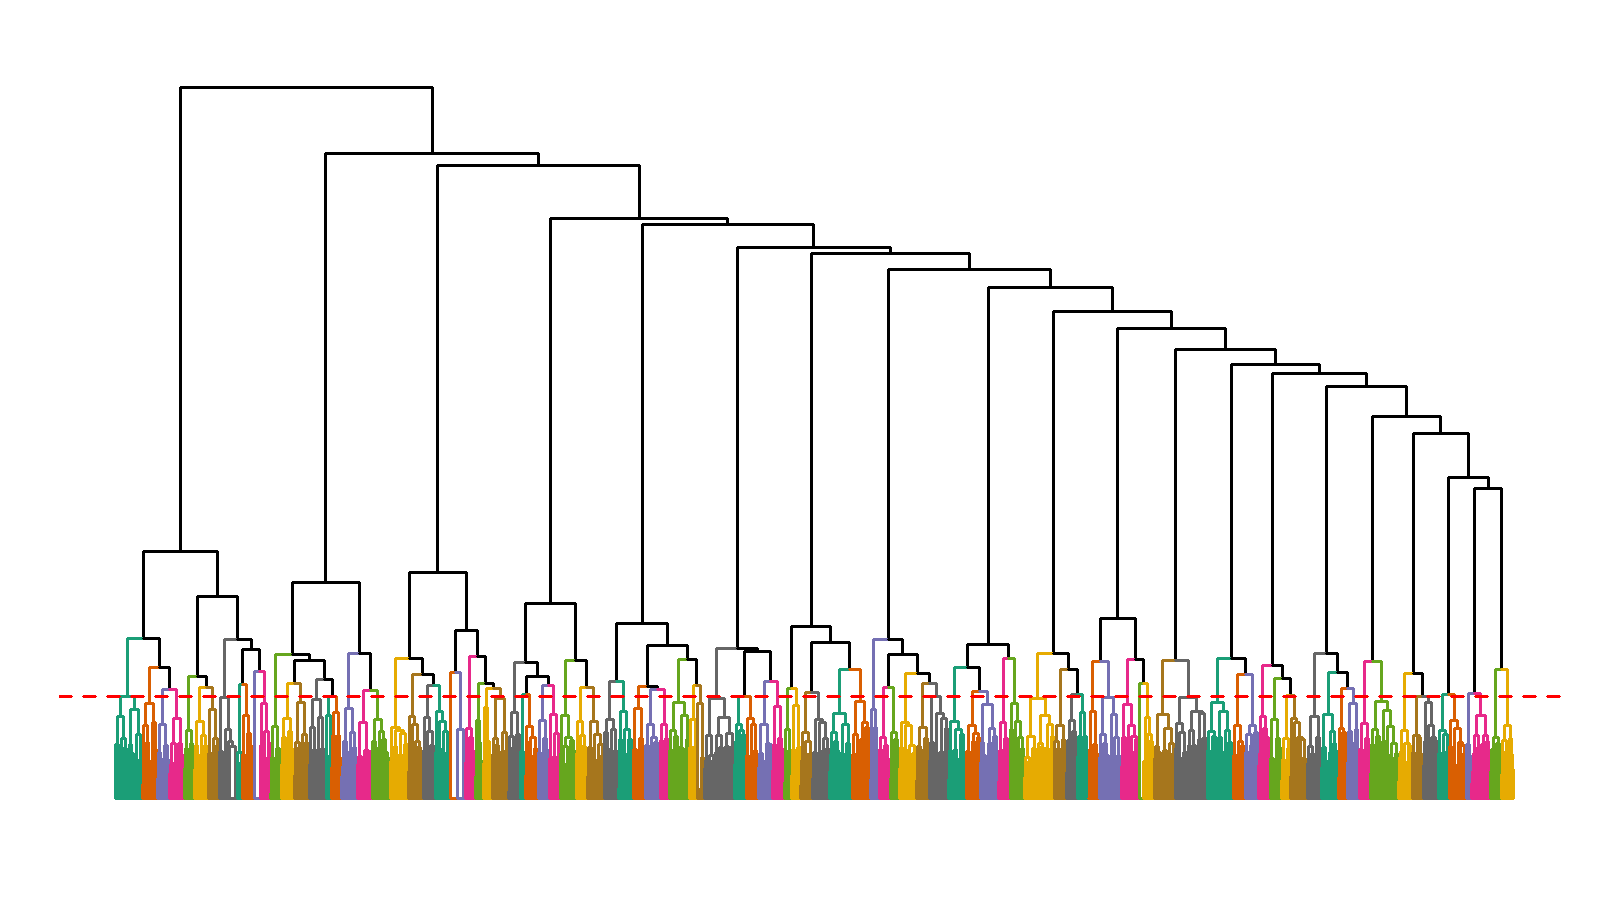
\includegraphics[width=1.0\textwidth]{Figs/Dend/all-branches-micro.png}
        \caption{c = 3, k = 102}
        \label{fig:dend-micro}
    \end{subfigure} 
     \begin{subfigure}[b]{0.5\textwidth}
        \centering
        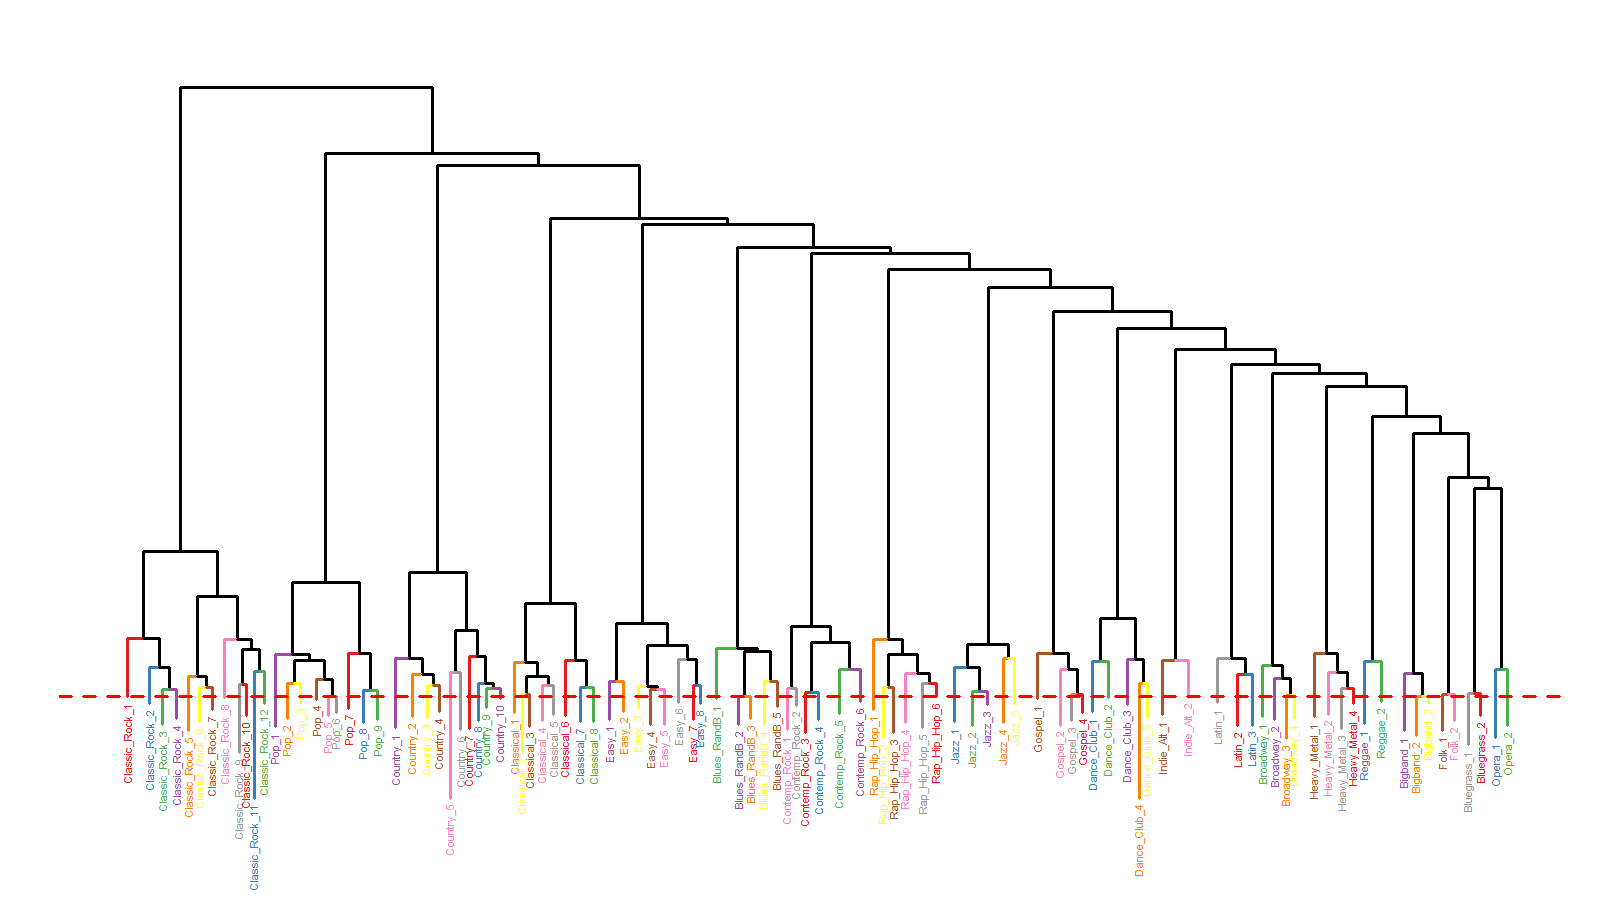
\includegraphics[width=1.0\textwidth]{Figs/Dend/all-branches-micro-labels.png}
        \caption{c = 3, k = 102}
        \label{fig:dend-micro-labels}
    \end{subfigure}
     \begin{subfigure}[b]{0.32\textwidth}
        \centering
        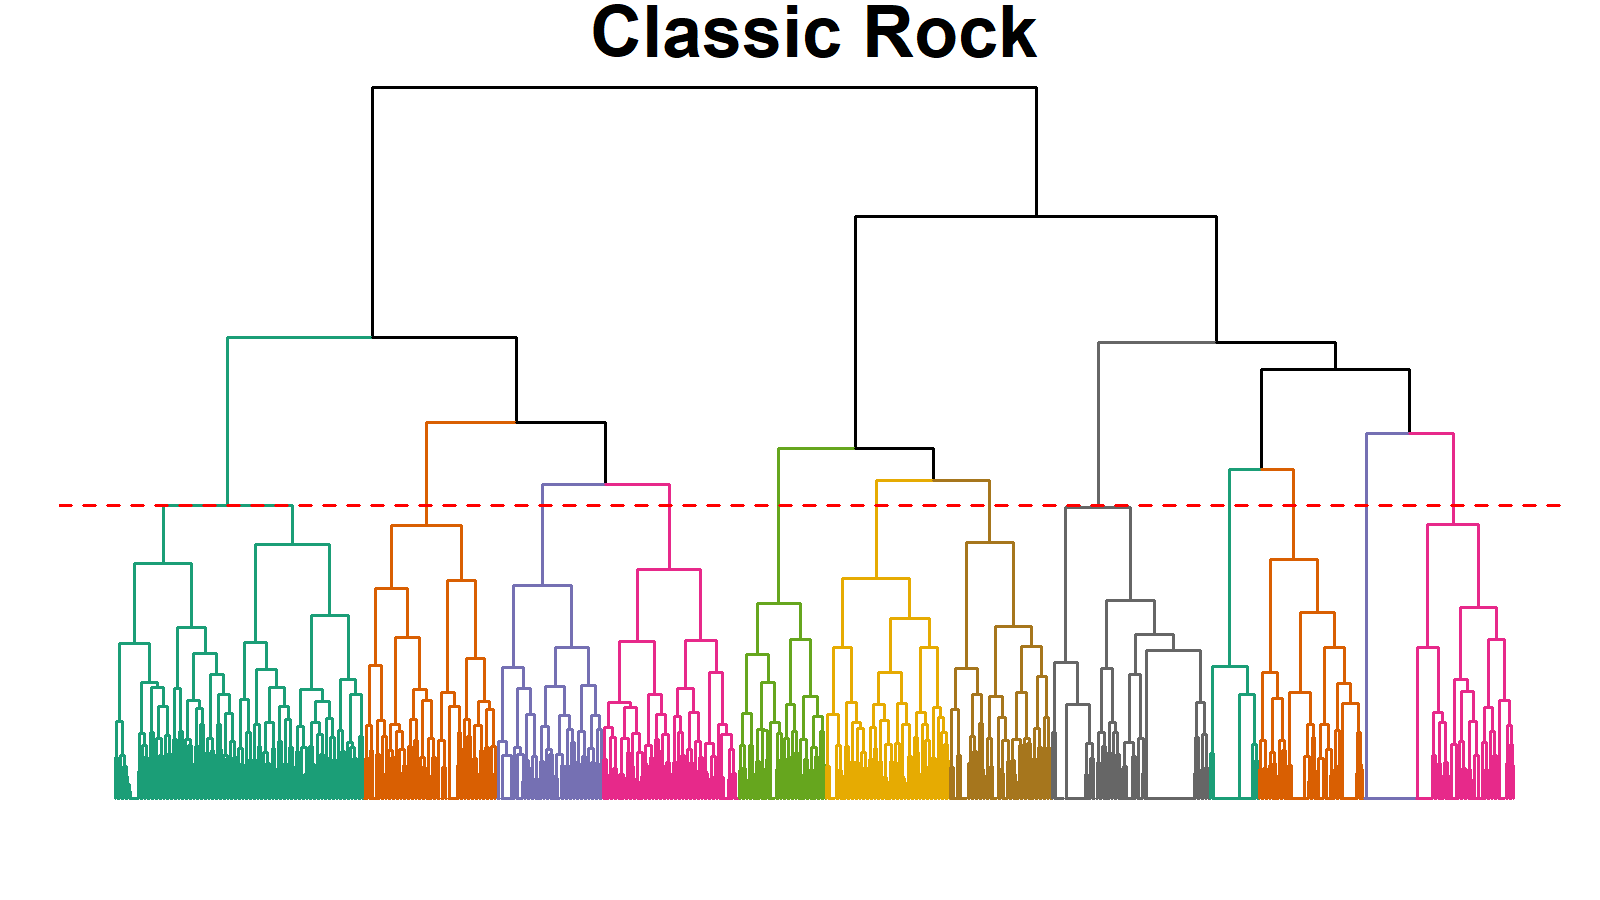
\includegraphics[width=1.0\textwidth]{Figs/Dend/classic-rock-branches.png}
        \caption{c = 3, k = 12}
        \label{fig:dend-micro-classic-rock}
    \end{subfigure} 
     \begin{subfigure}[b]{0.32\textwidth}
        \centering
        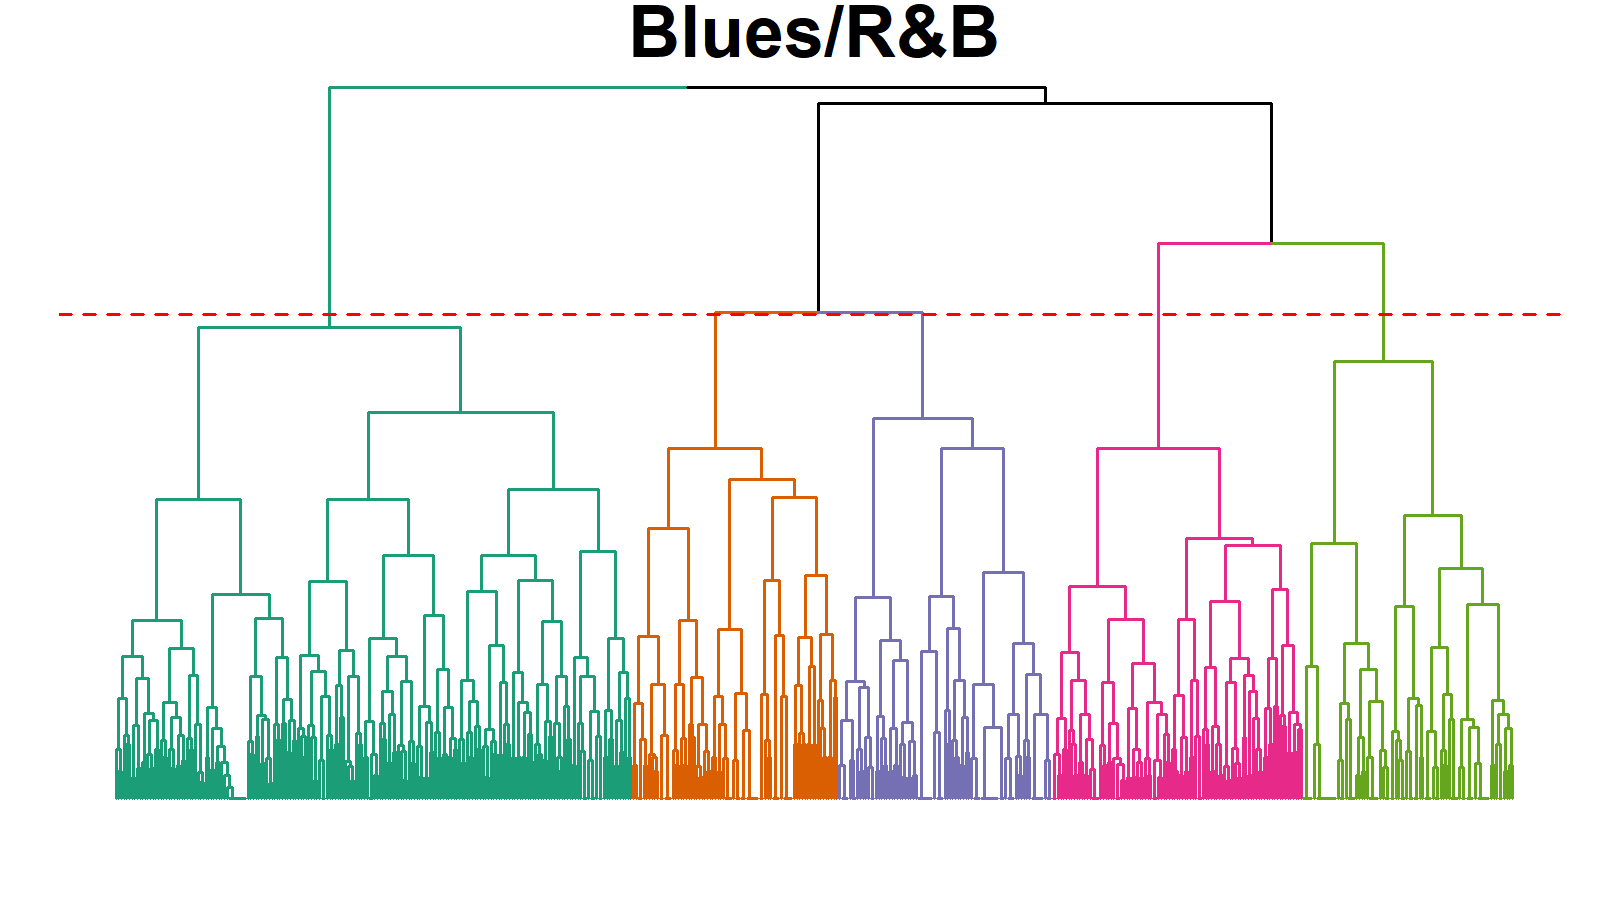
\includegraphics[width=1.0\textwidth]{Figs/Dend/blues-branches.png}
        \caption{c = 3, k = 5}
        \label{fig:dend-micro-blues}
    \end{subfigure}
     \begin{subfigure}[b]{0.32\textwidth}
        \centering
        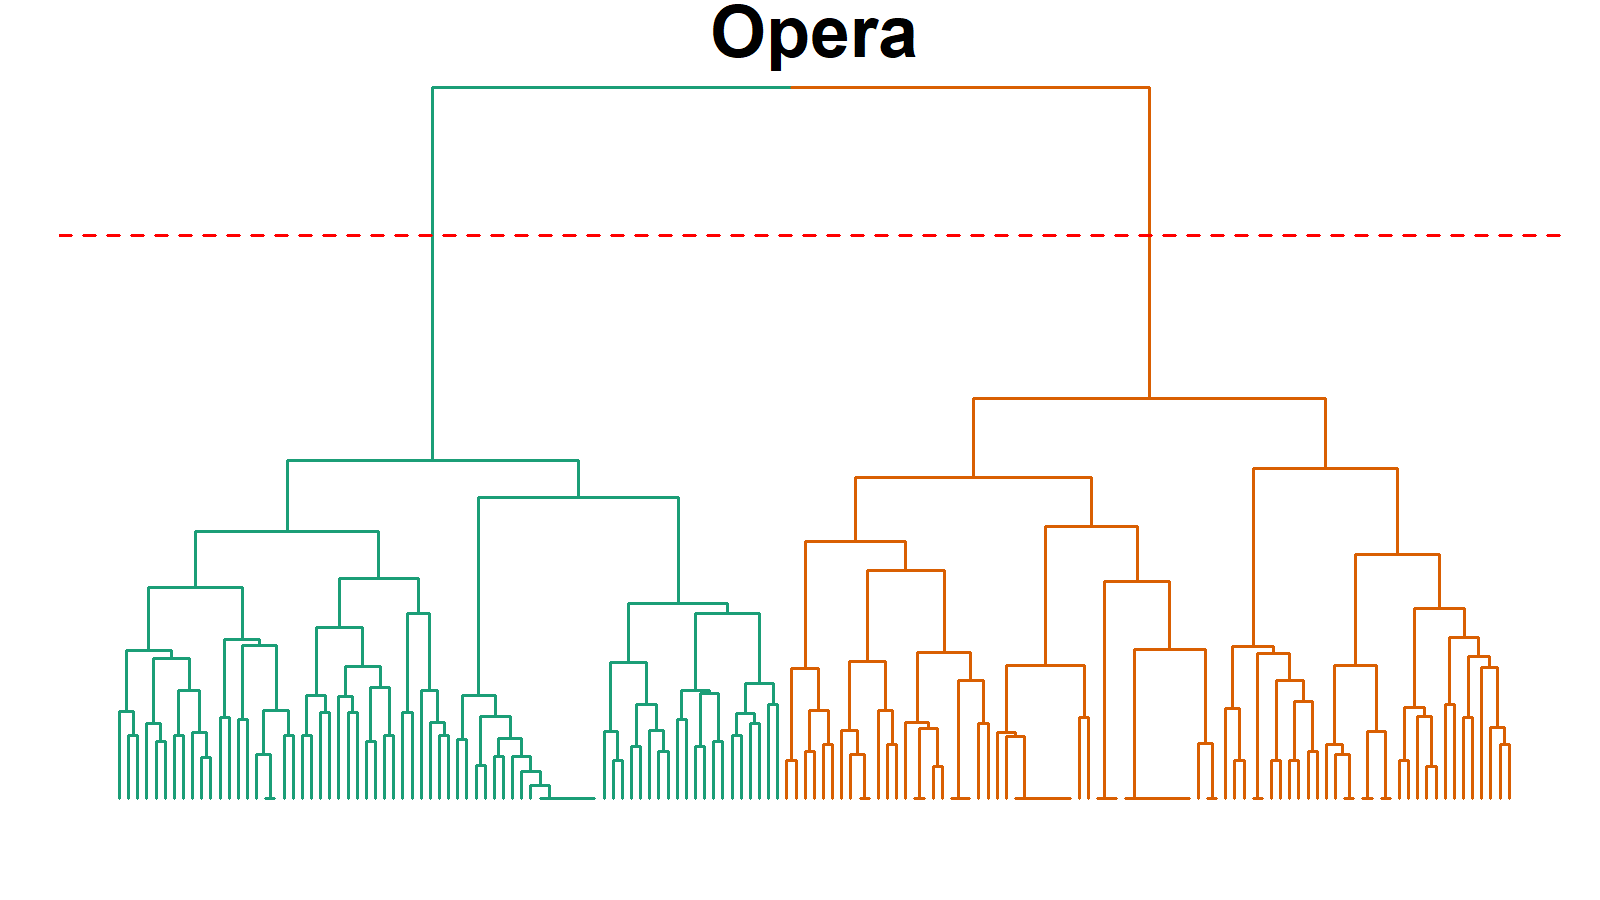
\includegraphics[width=1.0\textwidth]{Figs/Dend/opera-branches.png}
        \caption{c = 3, k = 2}
        \label{fig:dend-micro-opera}
    \end{subfigure}
    \caption{}
    \label{fig:dend}
 \end{figure}
 
The resulting partition has two interesting (and desirable) properties. First, the number of genre communities that \textit{people} belong to is deterministic, and it is given by the number of macro-genre labels they initially chose. Thus, link clustering preserves the cultural ego network degrees (omnivorousness by volume) of the people mode \citep{lizardo14}. Second, the number of micro-genres into which the macro-genres are split is {\em not} deterministic. Instead, it is data-driven (discovered or learned) and cannot be pre-specified in advance. It is a function of relational information implicit in the overlap structure of the cultural ego networks of people in the data. Thus, link community detection of the person-to-genre network allows us to go from  a situation starting with a person-to-genre network featuring a relatively small number of macro-genres and end up with an enlarged two-mode network with the same number of nodes in one mode (the people) but many more nodes in the other mode (the micro-genres). How many micro-genres ($N_m$) emerge is up to the analyst as it depends on where we ``cut'' the resulting clustering dendrogram. This will be somewhere in between $N_g \geq N_m \leq N_l$, where $N_g$ is the number of original (macro) genres and $N_l$ is the number of person-to-genre links.

\section{Analysis and Results}
\subsection{Discovering Micro-genre Communities in Real Data}
Let us see how this process works in real data. We will see that link clustering can uncover valid micro-genres. Recall that the data feature 2,263 people choosing up to 20 macro-genre labels. When strung out as an edgelist, this results in 9,216 person-to-genre connections in the data, the resulting $9216 \times 9,216$ matrix, containing Jaccard similarities among person-to-genre links sharing a node in either of the two modes, is then the input to an agglomerative hierarchical clustering algorithm using Ward's \citep{ward63} method. The hierarchical clustering process proceeds as follows. Initially  each person-to-genre link is initially assigned to its own community. Then, in the second time step, the pairs of links with the largest Jaccard similarities are put in the same clump. This continues at each time step, where pairs of links with the largest similarity are chosen, and their respective communities are merged. This process is repeated until all links belong to a single cluster. The history of the clustering process is then stored in a dendrogram, which encodes all the information on the hierarchical organization of the genre communities. The height of the dendrogram provides information about the strength of the genre communities. As we have seen, the highest levels reproduce the original macro-genres, while the lower levels uncover more focused micro-genres embedded within them. This is shown in Figure~\ref{fig:dend}. 

Figure~\ref{fig:dend-macro} shows that when we cut the dendrogram at a high level (e.g., $C = 8$), we reproduce the original twenty macro-genres we began with as the ``discovered'' link communities. Note that, as Figure~\ref{fig:dend-macro-labels} shows, the agglomerative link clustering procedure arranges the macro-genre levels roughly by their original popularity (number of person-to-genre links). From left to right, these are Classic Rock/Oldies, Pop/Top 40, Country, Classical, Easy Listening, Blues/R\&B, Contemporary Rock, Rap/Hip Hop, Jazz, Gospel, Dance/Club, Indie Alternative, Latin, Broadway/Musicals, Heavy Metal/Hard Rock, Reggae, Big Band, Folk, Bluegrass, and Opera. As shown in Figure~\ref{fig:dend-micro}, micro-genre communities are produced by cutting the link clustering dendrogram at a lower level. When we choose a cutoff value of $c = 3$ results in $k = 102$ micro-genre communities extracted from the original twenty macro-genre labels. Data scientists wring their hands when performing cluster analysis about choosing a cut value. One advantage of the link clustering approach is that we always know what we are doing because micro-genres are strictly nested within the original macro-genres. On the other hand, choosing a smaller cut value produces finer-grained micro-genres (perhaps at the expense of analytic tractability and interoperability), and selecting a higher value returns us to broader genre communities closer to the original macro-genre labels we began with (with the limiting case as shown in Figure~\ref{fig:dend-macro} being the original macro genre labels themselves). As Figure~\ref{fig:dend-micro-labels} shows, at any cut value $C$, the more popular macro-genres produce more micro-genre communities, while the less popular ones produce a smaller number. For instance, as shown in Figure~\ref{fig:dend-micro-classic-rock}, at $c = 3$, the macro-genre ``Classic Rock/Oldies'' (the leftmost set of branches in the dendrogram in Figure~\ref{fig:dend-macro}) is split (at the point at which the branches intersect the red dashed cut line) into $k_{(CR)} = 12$ distinct micro-variations, while, as Figure~\ref{fig:dend-micro-opera} shows, the macro-genre ``Opera" (the rightmost set of branches in the dendrogram in Figure~\ref{fig:dend-macro}) is split into only $k_{(Op)} = 2$  micro-genre communities. Figure~\ref{fig:dend-micro-blues} shows that ``Blues/R\&B'' falls somewhere in between, with $k_{(BRB)} = 5$  micro-genre communities uncovered.

Each cut point in the dendrogram will have a micro-genre size distribution $N$ associated with it. Lower cut points return a micro-genre size distribution dominated by many micro-genres with tiny ($N_{mg} < 10$) or trivial $N_{mg} = 2$ audiences. In this respect, although I have been using the labels ``macro'' and ``micro'' as if they referred to substantive or objective partitions, they are best interpreted as {\em relative} to a given classification level. Thus, micro-genres are ``micro'' relative to the usual (perhaps ``basic'' in Rosch's \citeyearpar{Rosch1978-ue} sense) level of vague macro-genre labels that populate most arts participation surveys. But these may be micro, as we will see, relative to the (logics, discourses, schemas) meta-groupings that we generate when applying the usual suite of statistical and data reduction techniques (e.g., such as ``highbrow'' or ``Folk"). Further, at any given classification level, further micro-genres will be nested within any given micro-partition. In this way, micro-genre communities reflect a substantively valid way in which people partition the cultural world, whereby there is always the possibility of making finer-grained distinctions within fine-grained distinctions (e.g., ``old school rap," ``1980s old school rap,", ``early 1980s old school rap," and the like). 

Ultimately, there is no magical ``right'' answer here, but for analytic purposes $c = 3, k = 102, max(N_{mg}) = X, min(N_{mg}) = Y$ is sufficiently fine-grained to showcase the analytic advantages of the micro-genre approach. The resulting size distribution is shown in Figure~\ref{fig:size-dist}. The main panel shows the micro-genre communities chosen by 75 or more people, and the inset shows the entire size distribution. micro-genre communities are named according to the original macro-genre label, followed by a number. As the figure shows, the largest micro-genre communities in the data pertain to micro-variants of Indie/Alternative Rock, Contemporary Rock, Reggae, Classic Rock, Blues/R\&B, and Gospel. 

 \begin{figure}[ht!]
 \centering
 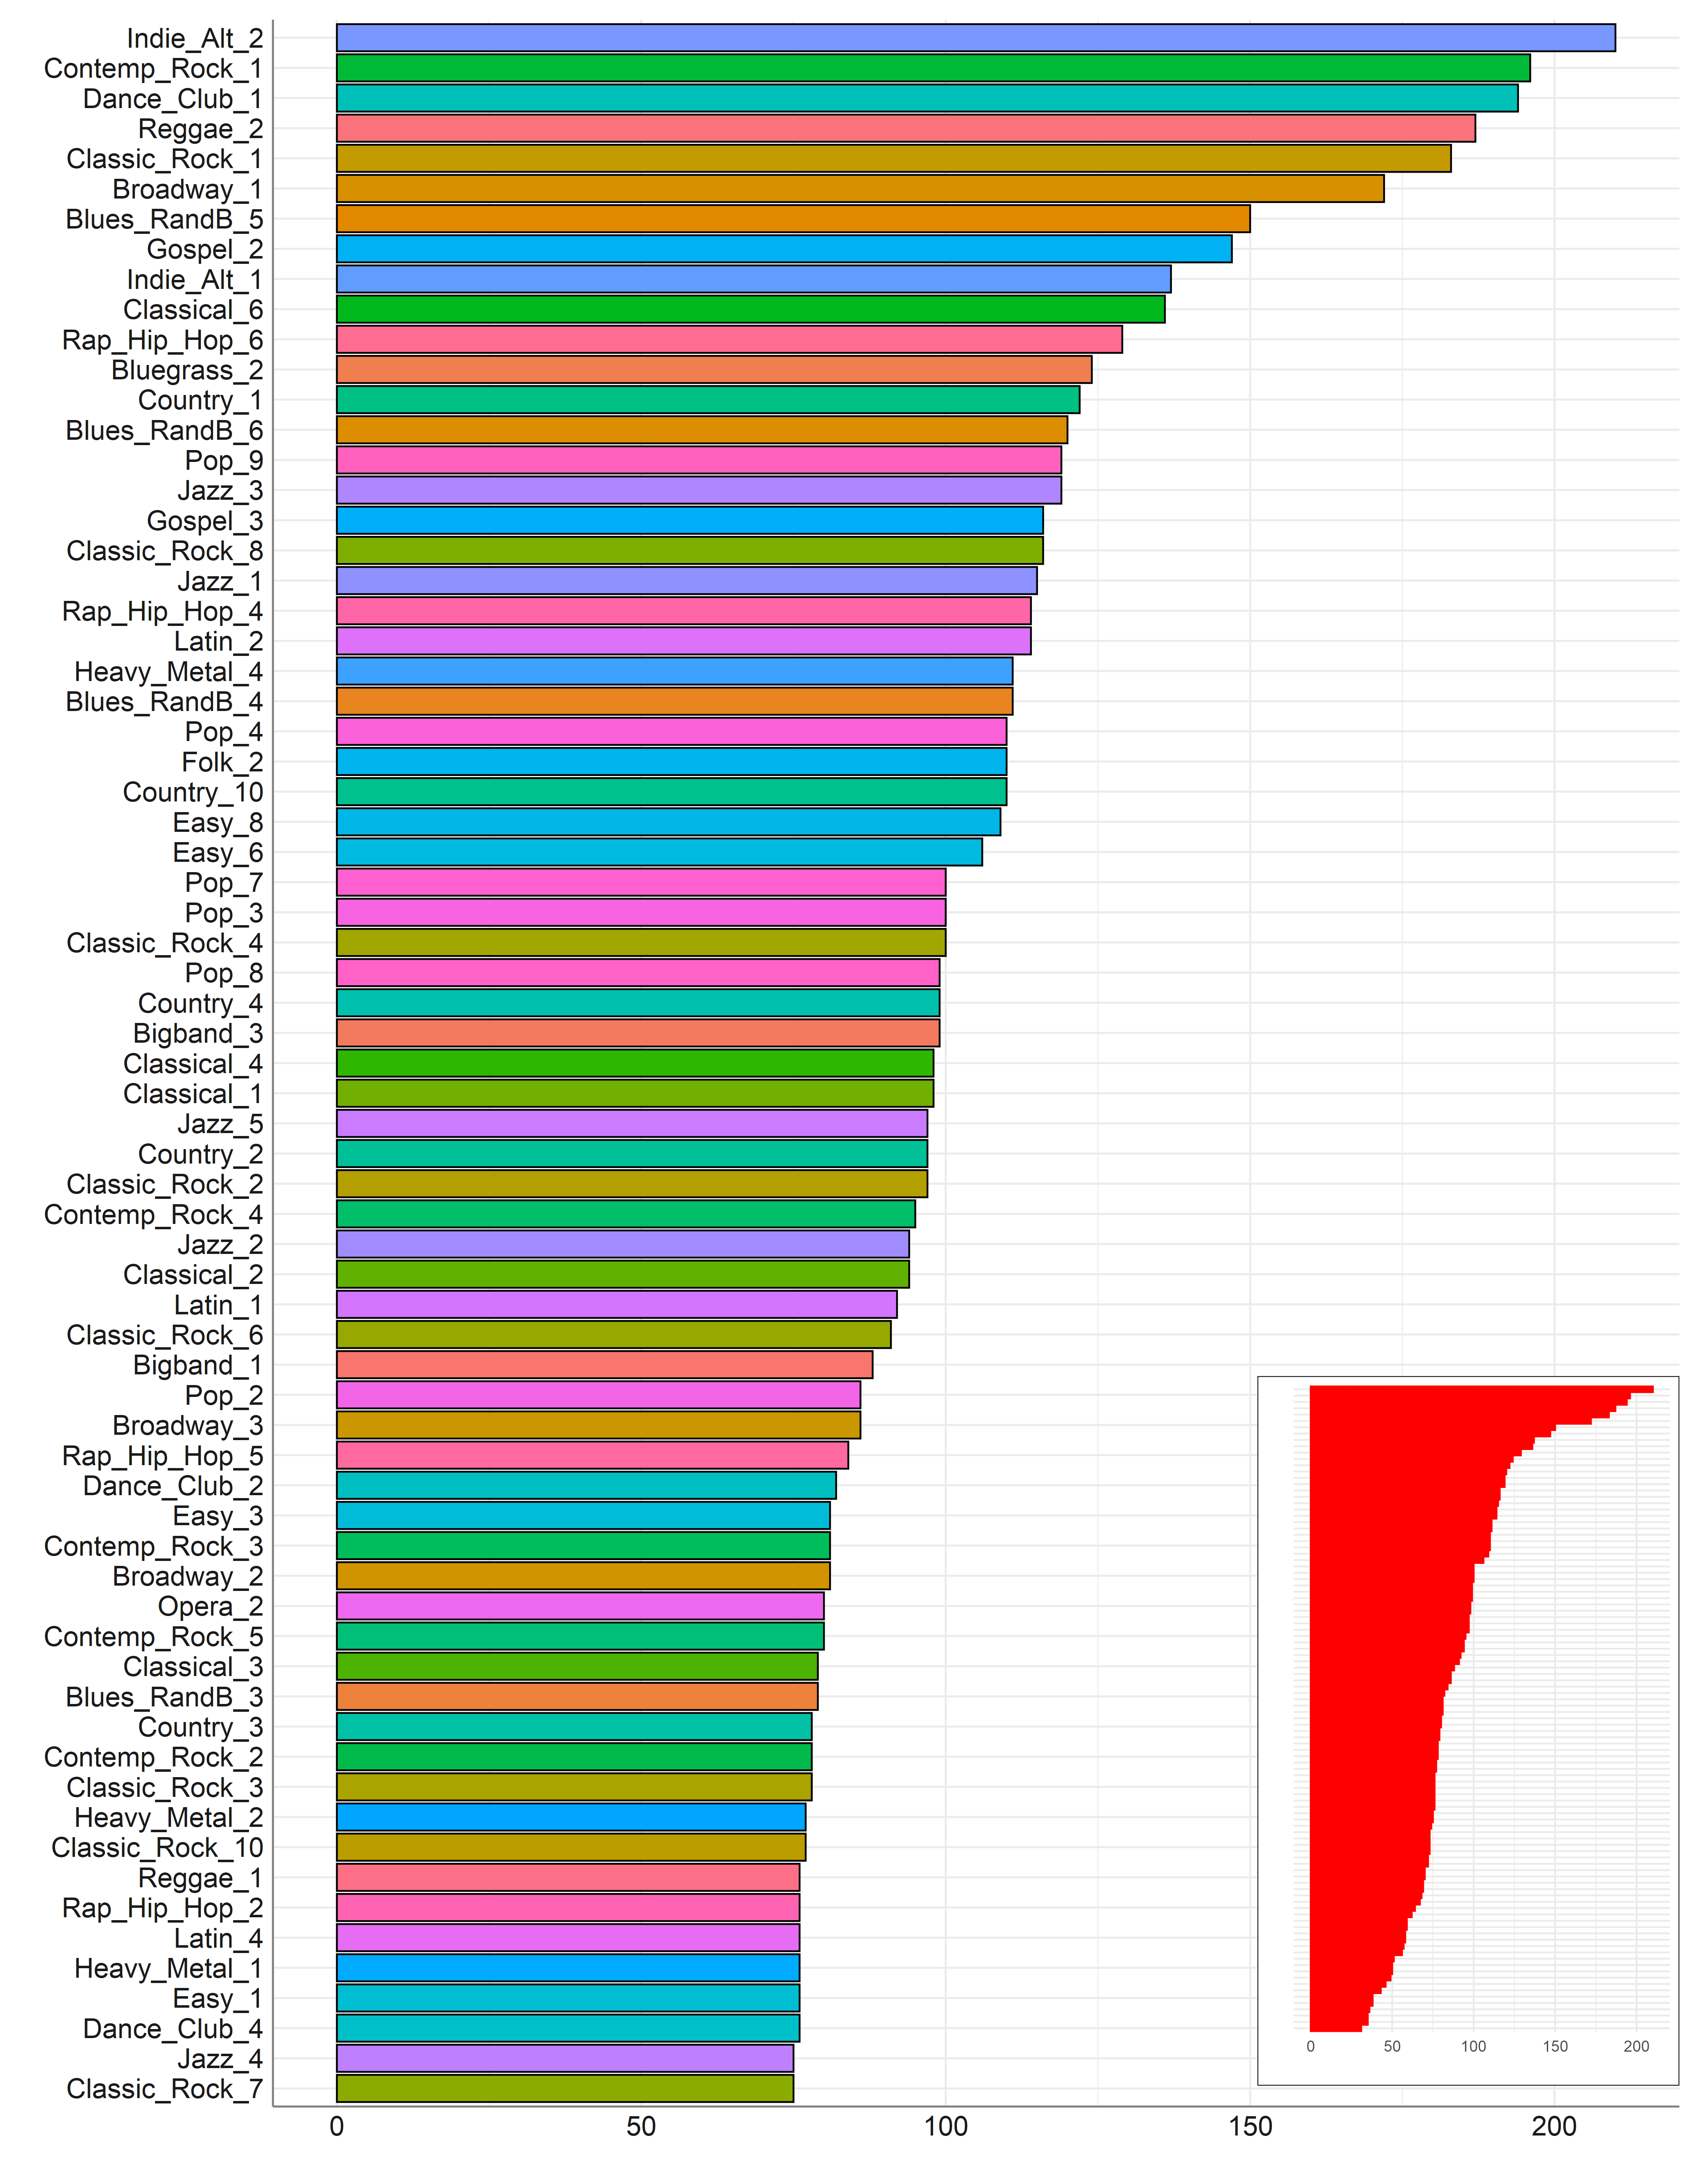
\includegraphics[width=0.7\textwidth]{Figs/Link Clust/micro-genre-size-dist.png}
 \caption{}
  \label{fig:size-dist}
 \end{figure}
 
\subsection{What Micro-Genre Communities Reveal}
\subsubsection{Hidden Dimensionality}
So what do we learn about people's tastes and about the micro-genres themselves after subjecting our data to link clustering? Comparing the answers we get from applying a standard, relatively undemanding (in terms of statistical assumptions foisted upon the data), namely, Principal Components Analysis, to the original and link-clustered cultural network data (hereafter OD, and LCD, respectively) can be illuminating in this respect. Particularly in terms of showing what is revealed by the link clustering in exposing the hidden relationality in the data and in what ways relying on vague macro-genre levels leads us astray both substantively and theoretically.

\begin{figure}[ht!]
    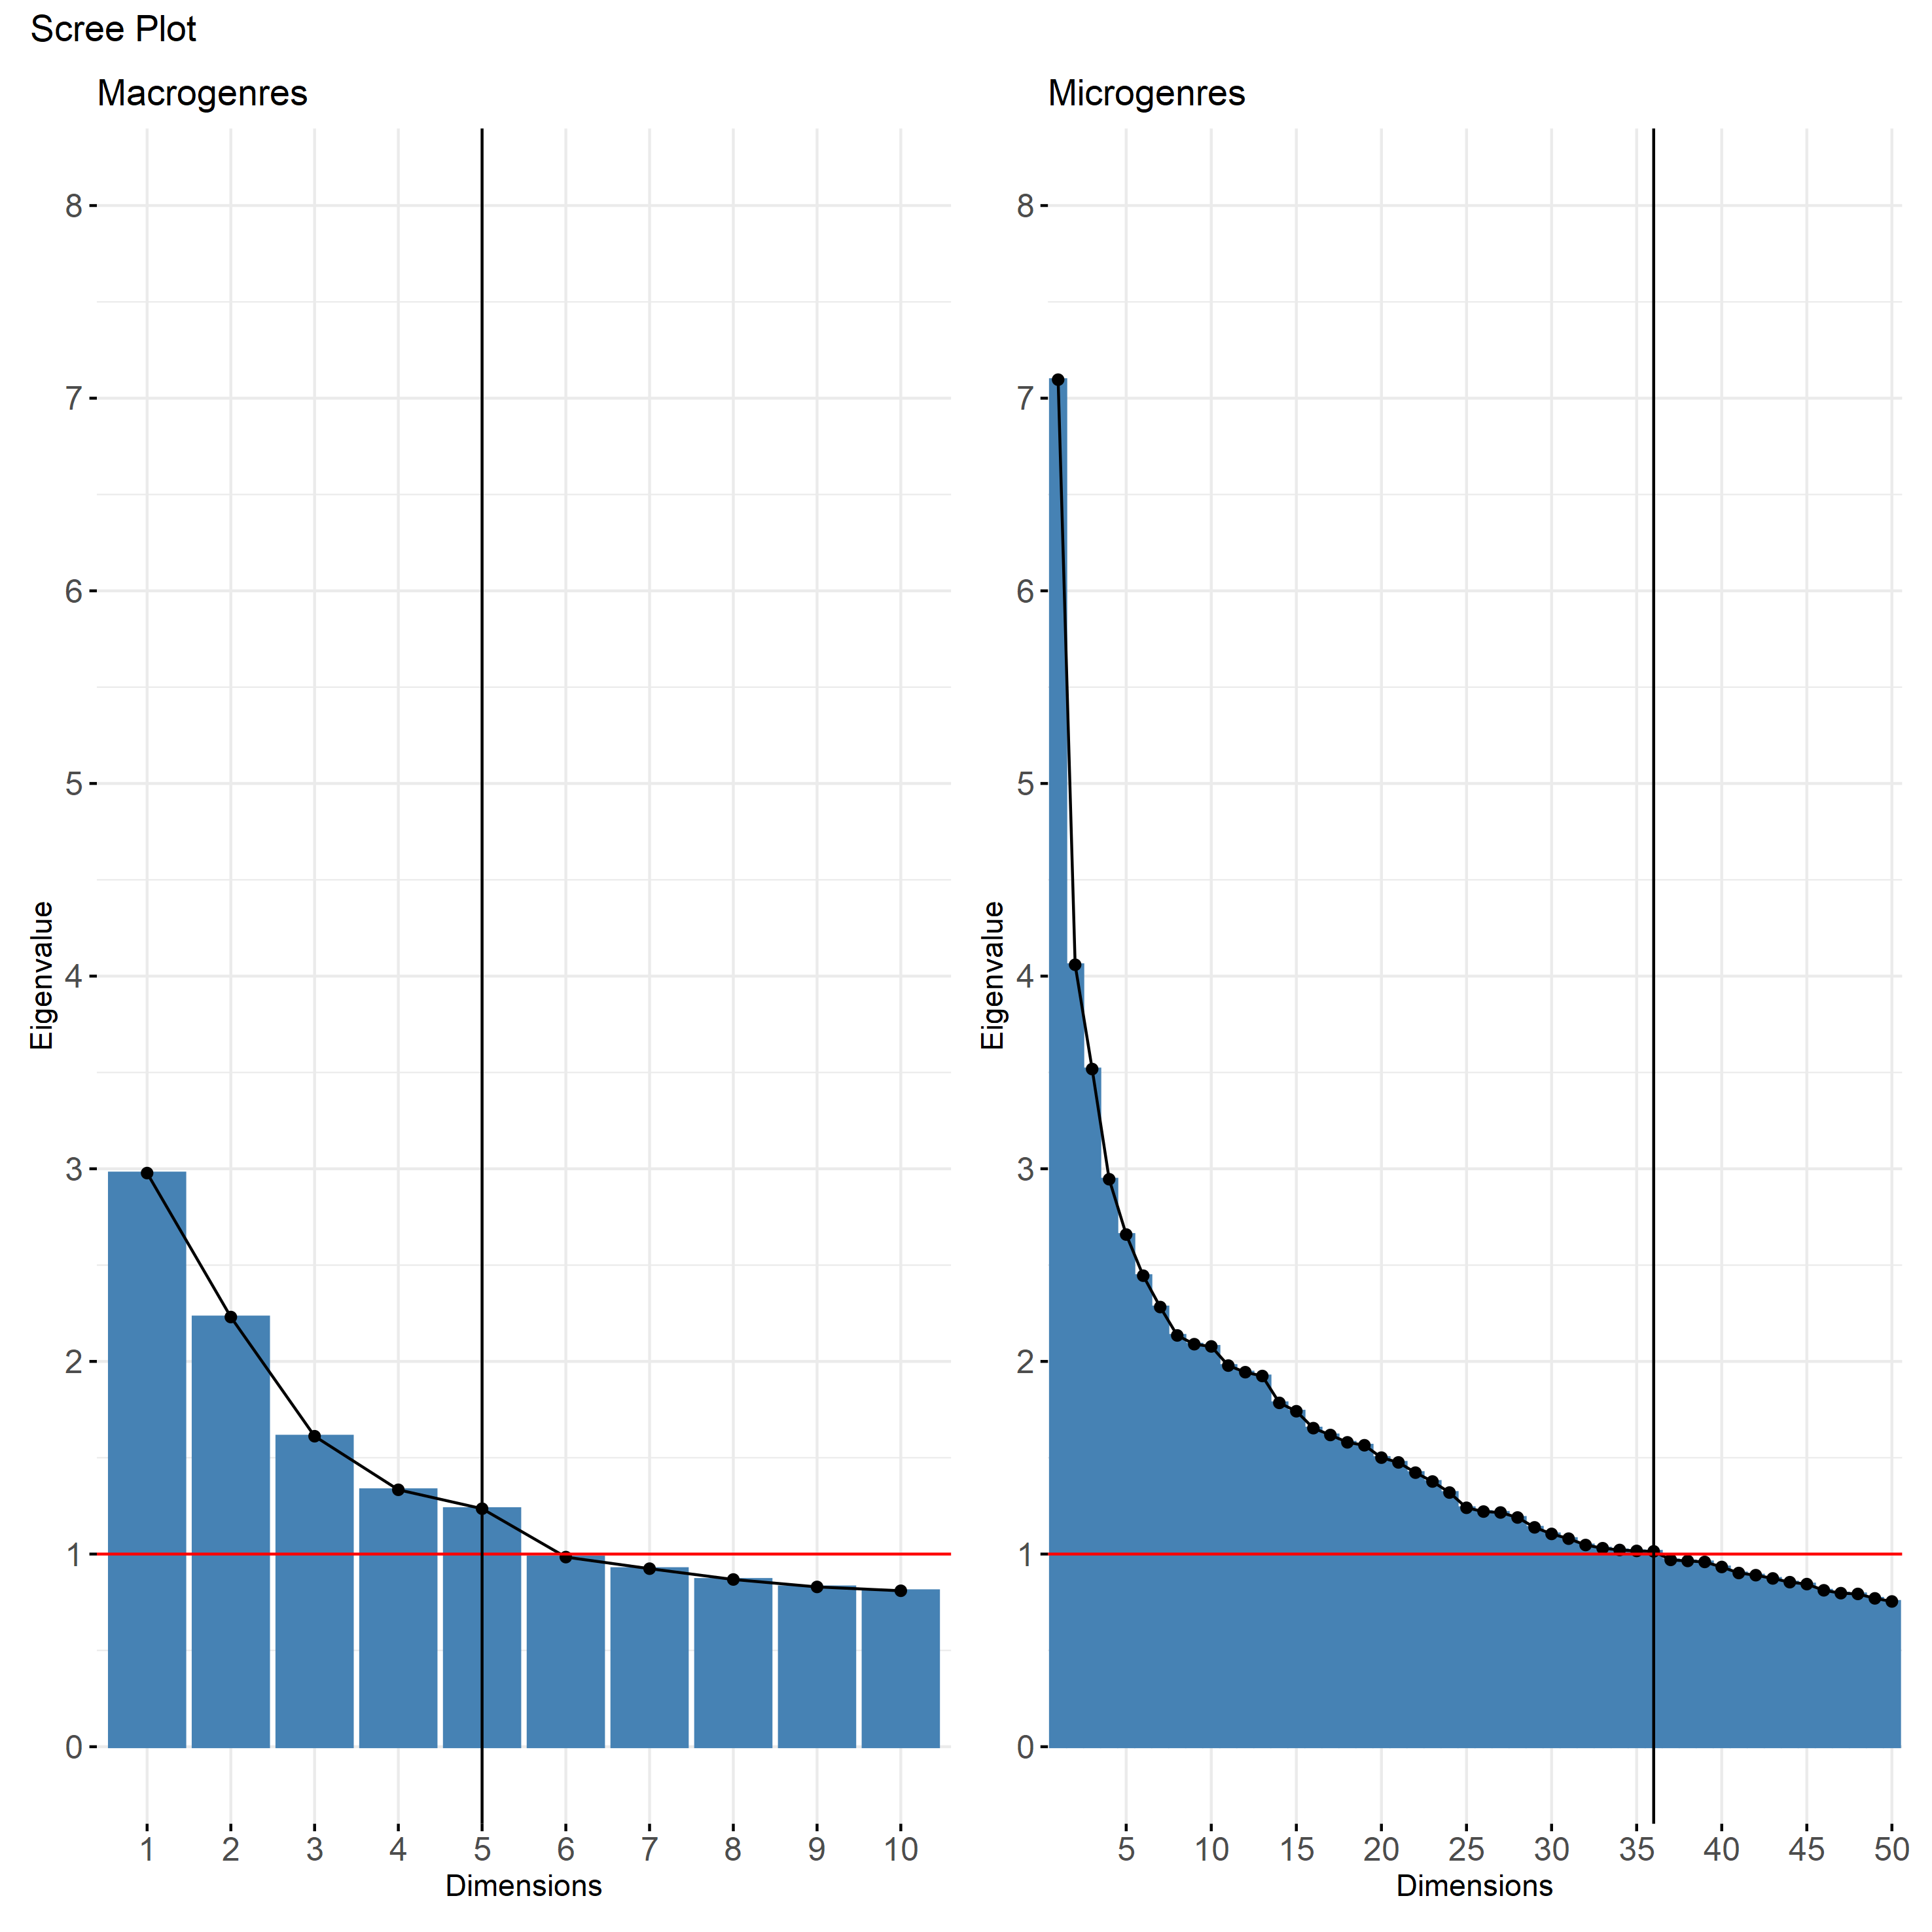
\includegraphics[width=1.0\textwidth]{Figs/Link Clust/macro-v-micro-pca-eig.png}
    \caption{}
    \label{fig:eig}
 \end{figure}

The first---perhaps already evident---thing we learn is that macrogenre labels hide underlying multidimensionality in cultural taste data, which the link clustering reveals. To show this, Figure \ref{fig:eig} shows the scree plot of the PCA analysis of the OD and the LCD. In the figure, the size of the eigenvalue is shown on the y-axis; the order (first, second, third, and so forth) of the corresponding eigenvalue is shown on the x-axis. The vertical red line going across the plot corresponds to the value on the y-axis where $\lambda = 1$. The black vertical line separates the eigenvalues for which $\lambda >= 1$ (on the left side of the plot) from those for which $\lambda < 1$ (on the right side of the plot). Using the rule of thumb that the number of eigenvalues for which $\lambda > 1$ point to significant dimensions of variation in the data, the PCA on the OD suggests the relevance of perhaps four dimensions that we may want to consider (usually, most analysts stick to the first two). The corresponding scree plot for the LCD reveals upwards of {\em twenty-five} dimensions that could be relevant. 

The first lesson we learn is that {\em macro-genre labels hide relevant dimensions of genre-level (and thus potential person-level) of differentiation in the data}. As we will see next, the artificial lower-dimensionality of the data considered by relying on macro-genre levels leads to substantively misleading answers to our questions.  

\subsubsection{Misleading Answers to Substantive Questions}
 What does the dimension-reduction analysis reveal substantively? Figures \ref{fig:macro-pca} and \ref{fig:micro-pca} show the result of ``classifying'' the genres using the first four dimensions of the PCA on the OD and the first twenty-five dimensions of the PCA on the LCD. In the figures, genres are classified using a ``hybrid'' (hierarchical/k-means) clustering of the (Euclidean) genre distance matrix in four-dimensional space (for the OD) and twenty-five-dimensional space (for the LCD). The number of clusters corresponds to the number of dimensions in the space; four macro-genre clusters ($k_{MG}$) and twenty-five micro-genre clusters ($k_{mg}$). After clustering, macro and micro-genres are re-embedded into two-dimensional space using their respective scores along the first two Principal Coordinates. 
 
\begin{figure}[ht!]
     \begin{subfigure}[b]{1.0\textwidth}
        \centering
        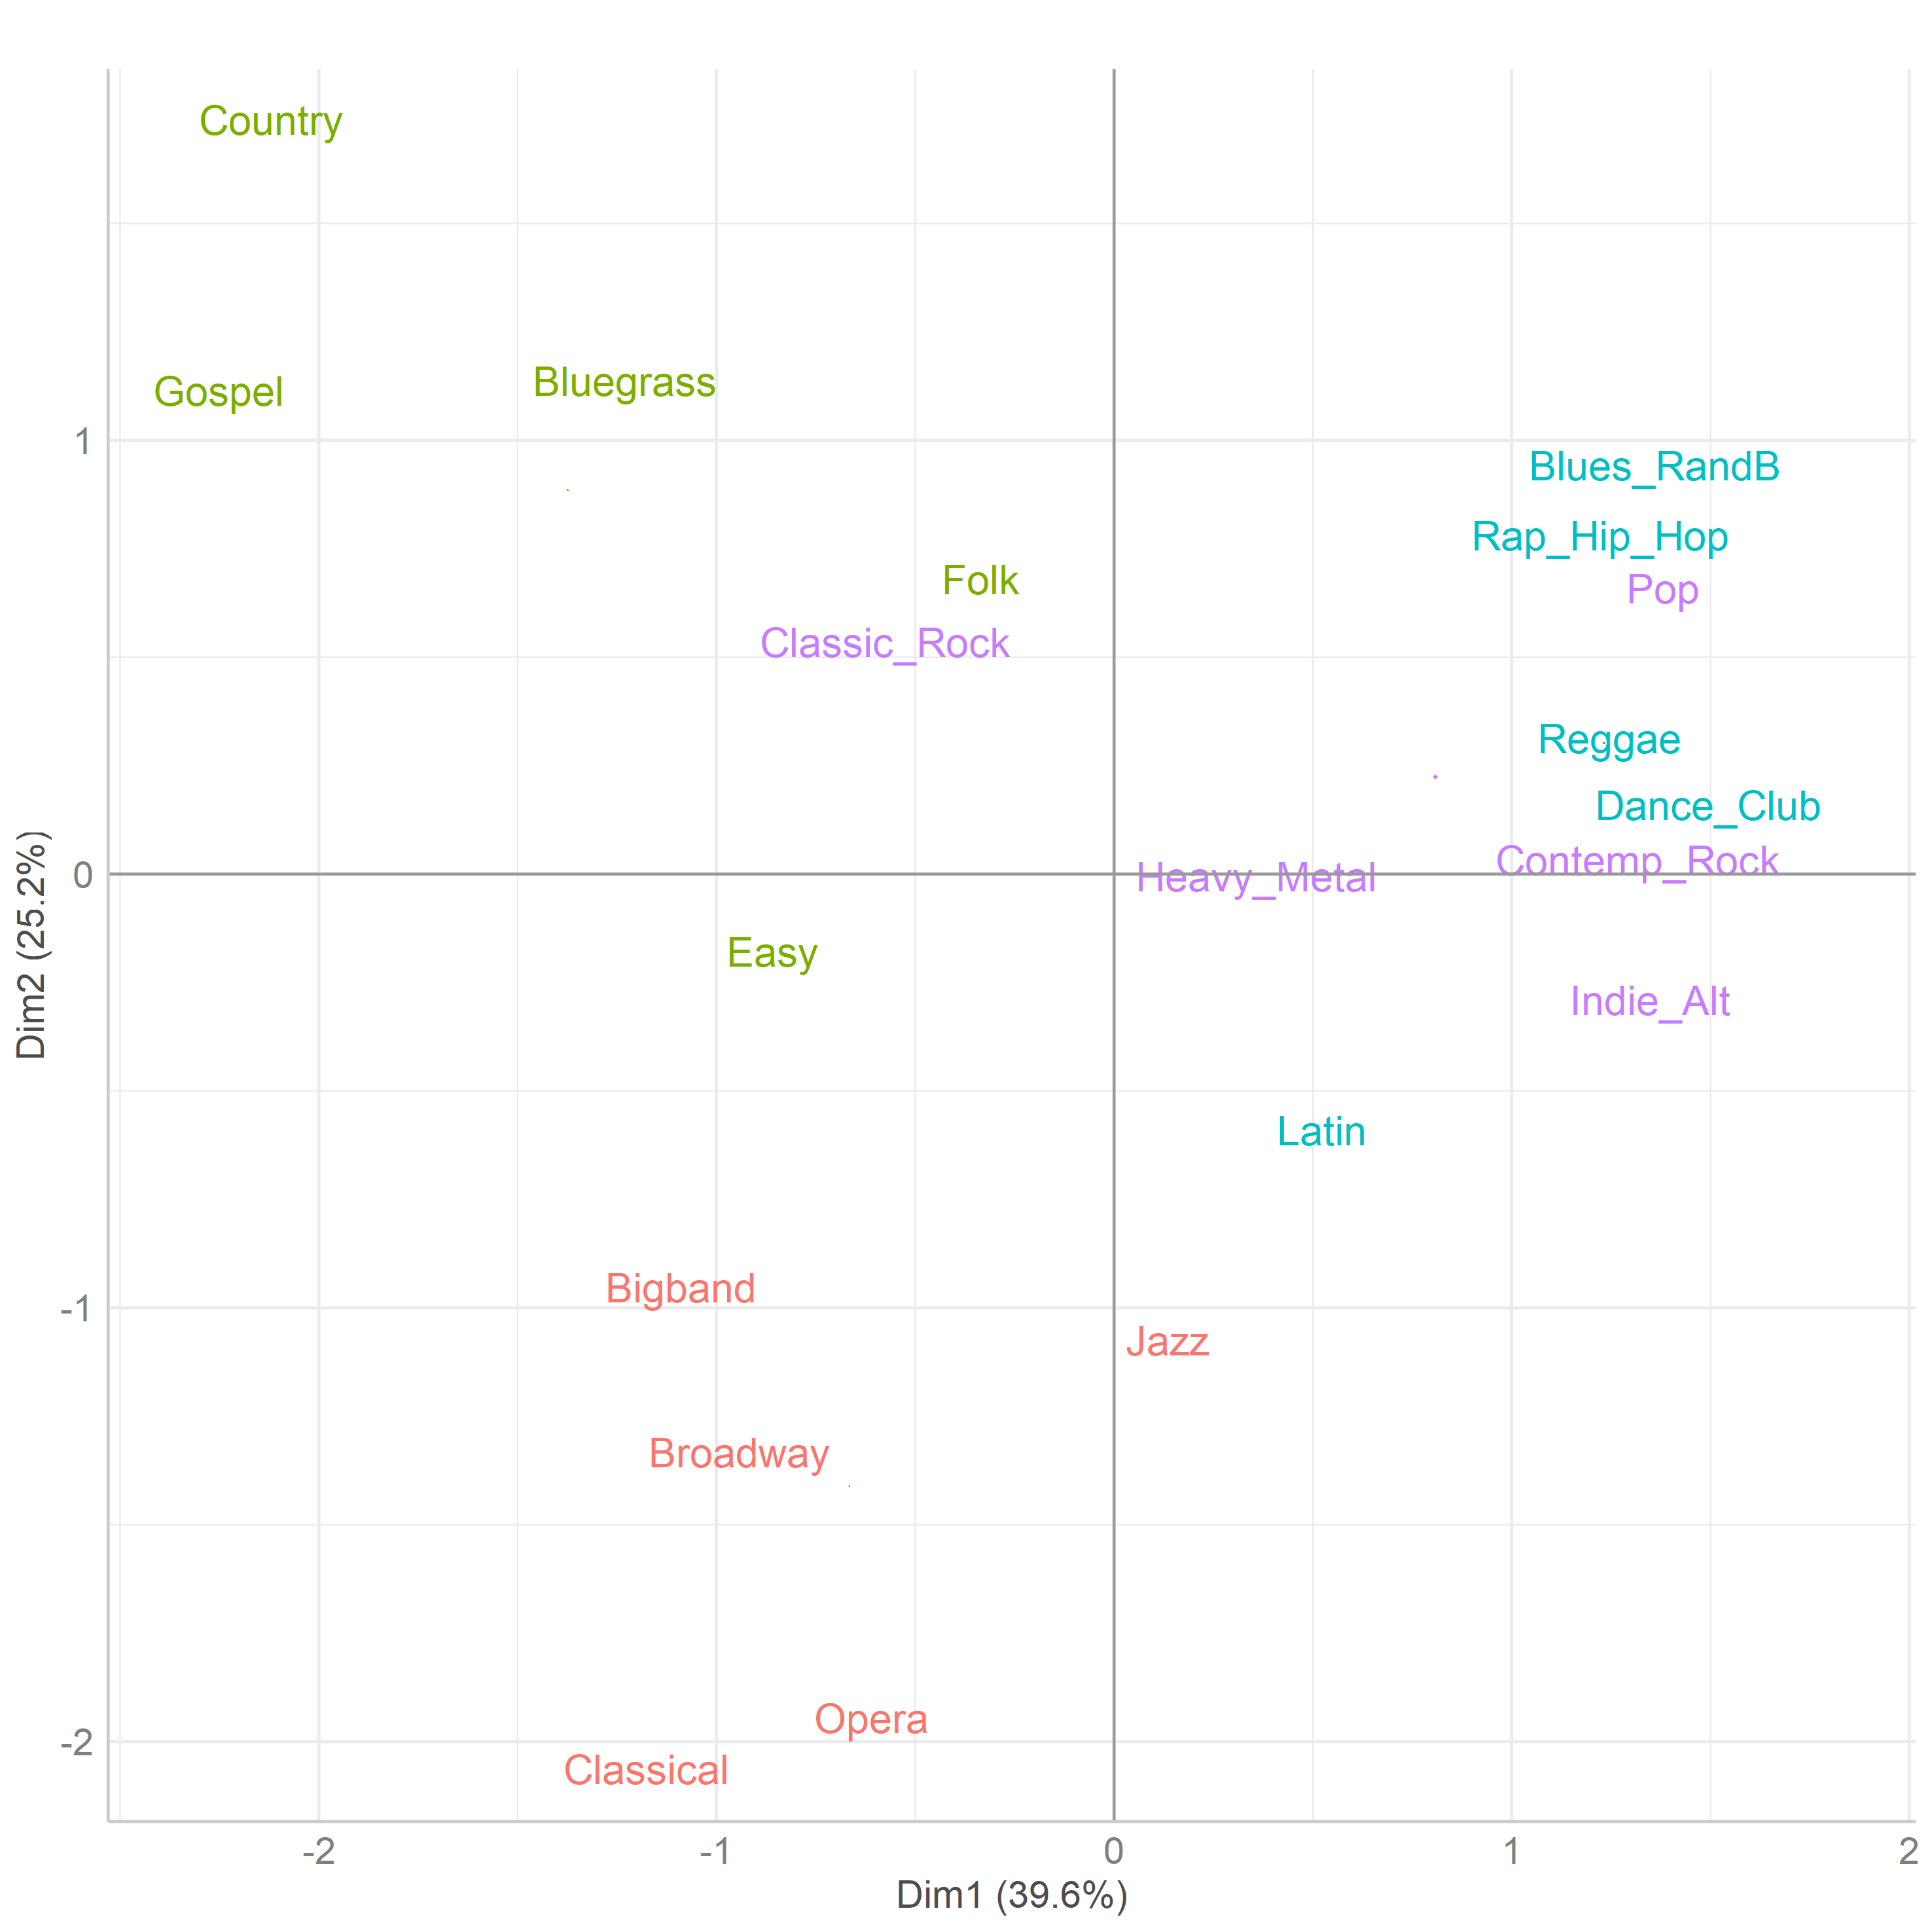
\includegraphics[width=0.6\textwidth]{Figs/Link Clust/macro-pca-clust.png}
        \caption{}
        \label{fig:macro-pca}
    \end{subfigure} 
     \begin{subfigure}[b]{1.0\textwidth}
        \centering
        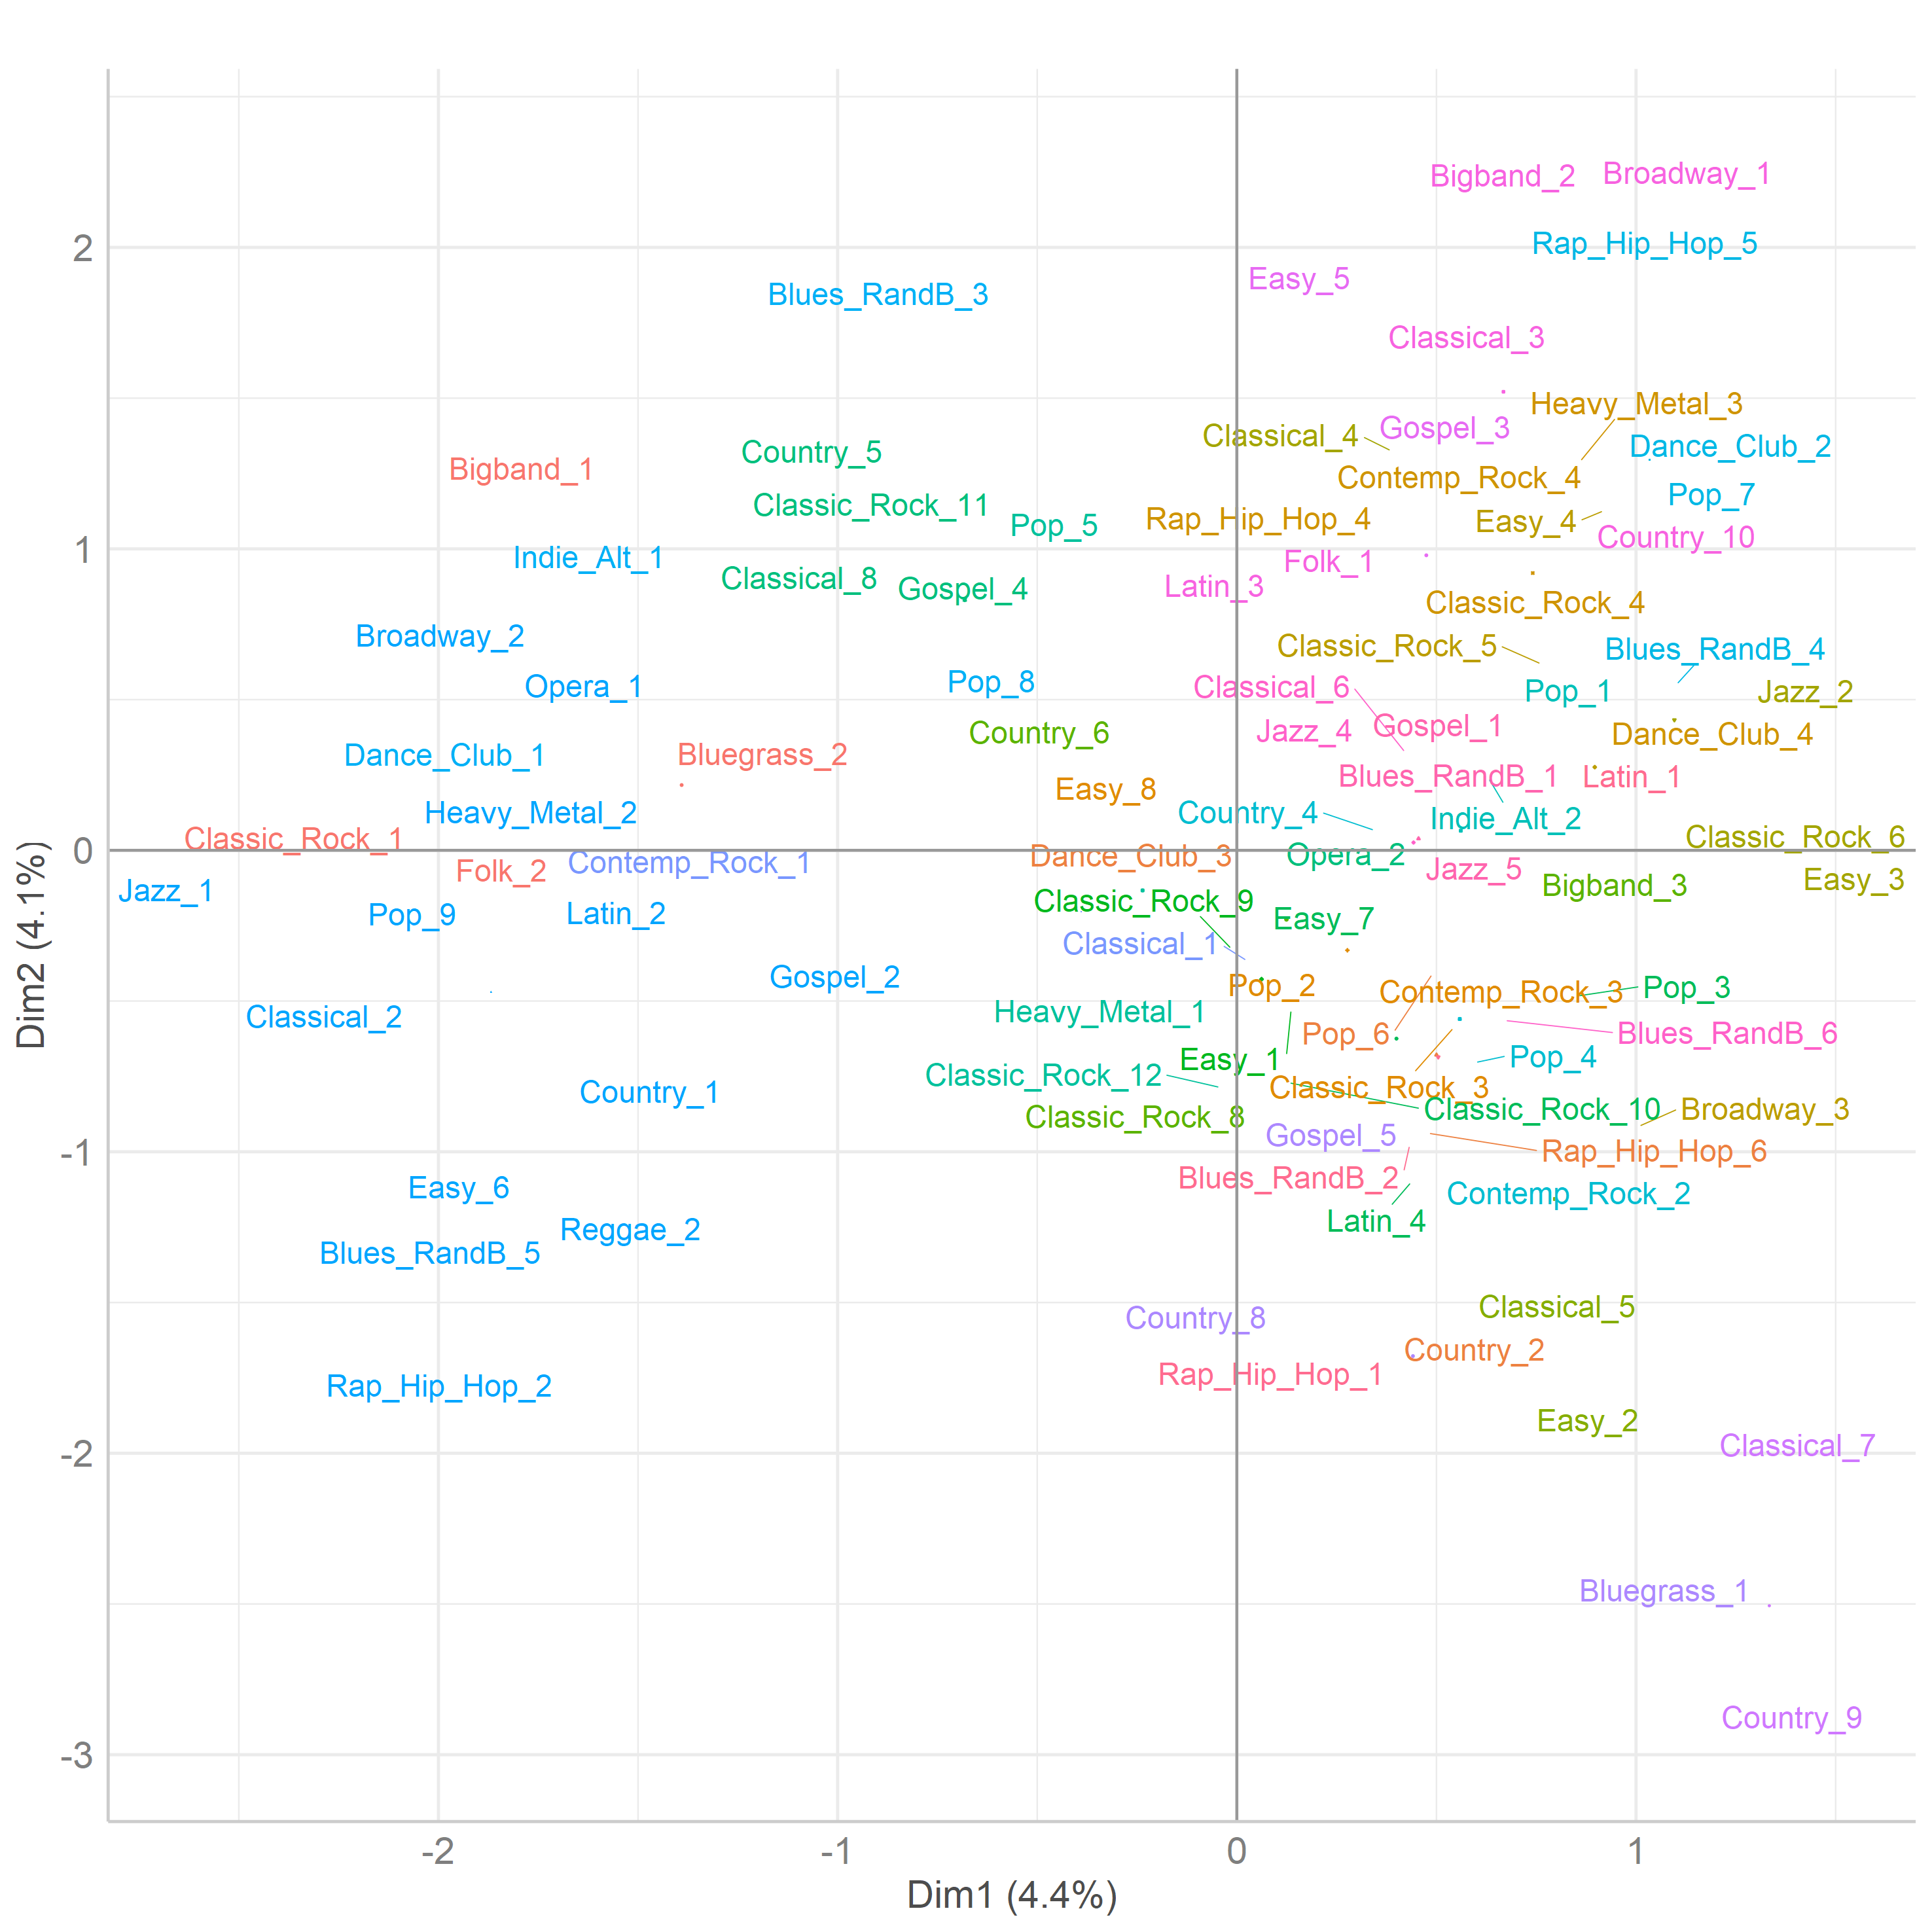
\includegraphics[width=0.6\textwidth]{Figs/Link Clust/micro-pca-clust.png}
        \caption{}
        \label{fig:micro-pca}
    \end{subfigure} 
    \caption{}
    \label{fig:macro-v-micro-pca}
 \end{figure}
 
 Figure~\ref{fig:macro-pca} suggests that a two-dimensional space does a good job of representing distinctions between macro-genres (accounting for about 65\% of the variance). Moreover, the macro-genre clusters correspond to the usual logics or discourses that populate many studies in the sociology of taste. On the upper-left, we have a variety of ``folk'' genres, including Country, Gospel, Bluegrass, and the eponymous Folk (with ``Easy'' as a boundary macrogenre). On the lower-left, we have the usual set of ``highbrow'' genres (with Jazz as a boundary macrogenre). On the right, we have the standard set of ``Pop/Industry'' macrogenres, perhaps partitioned, in the four-cluster solution, into ``Rock/Pop" (the varieties of Rock and Roll, with ``Classic Rock/Oldies as a boundary macrogenre) and ``Afro/Pop" (Rap, Reggae, Blues) variants (with ``Latin/Spanish" as a boundary macrogenre). 
 
 Suppose we follow the now well-established ``structuralist'' approach to interpreting these types of embeddings of cultural objects as a space governed by binary oppositions popularized by Bourdieu \citeyearpar{bourdieu84}. In that case, we might say that the first dimension separates or opposes Highbrow and Folk discourses to Pop/Industry logics. The second dimension opposes the (perhaps high-status) highbrow discourse to the perhaps lower-status folk discourse. The fact that Pop/Industry genres are less differentiated on this second, seemingly status-focused dimension might indicate less relevance of status distinctions among these macro-genres. This is all consistent with the usual story of the persistence of these broad meta-macro-genre distinctions and oppositions over time (e.g., in the case of the U.S.) or across national settings. 

\begin{figure}[ht!]
    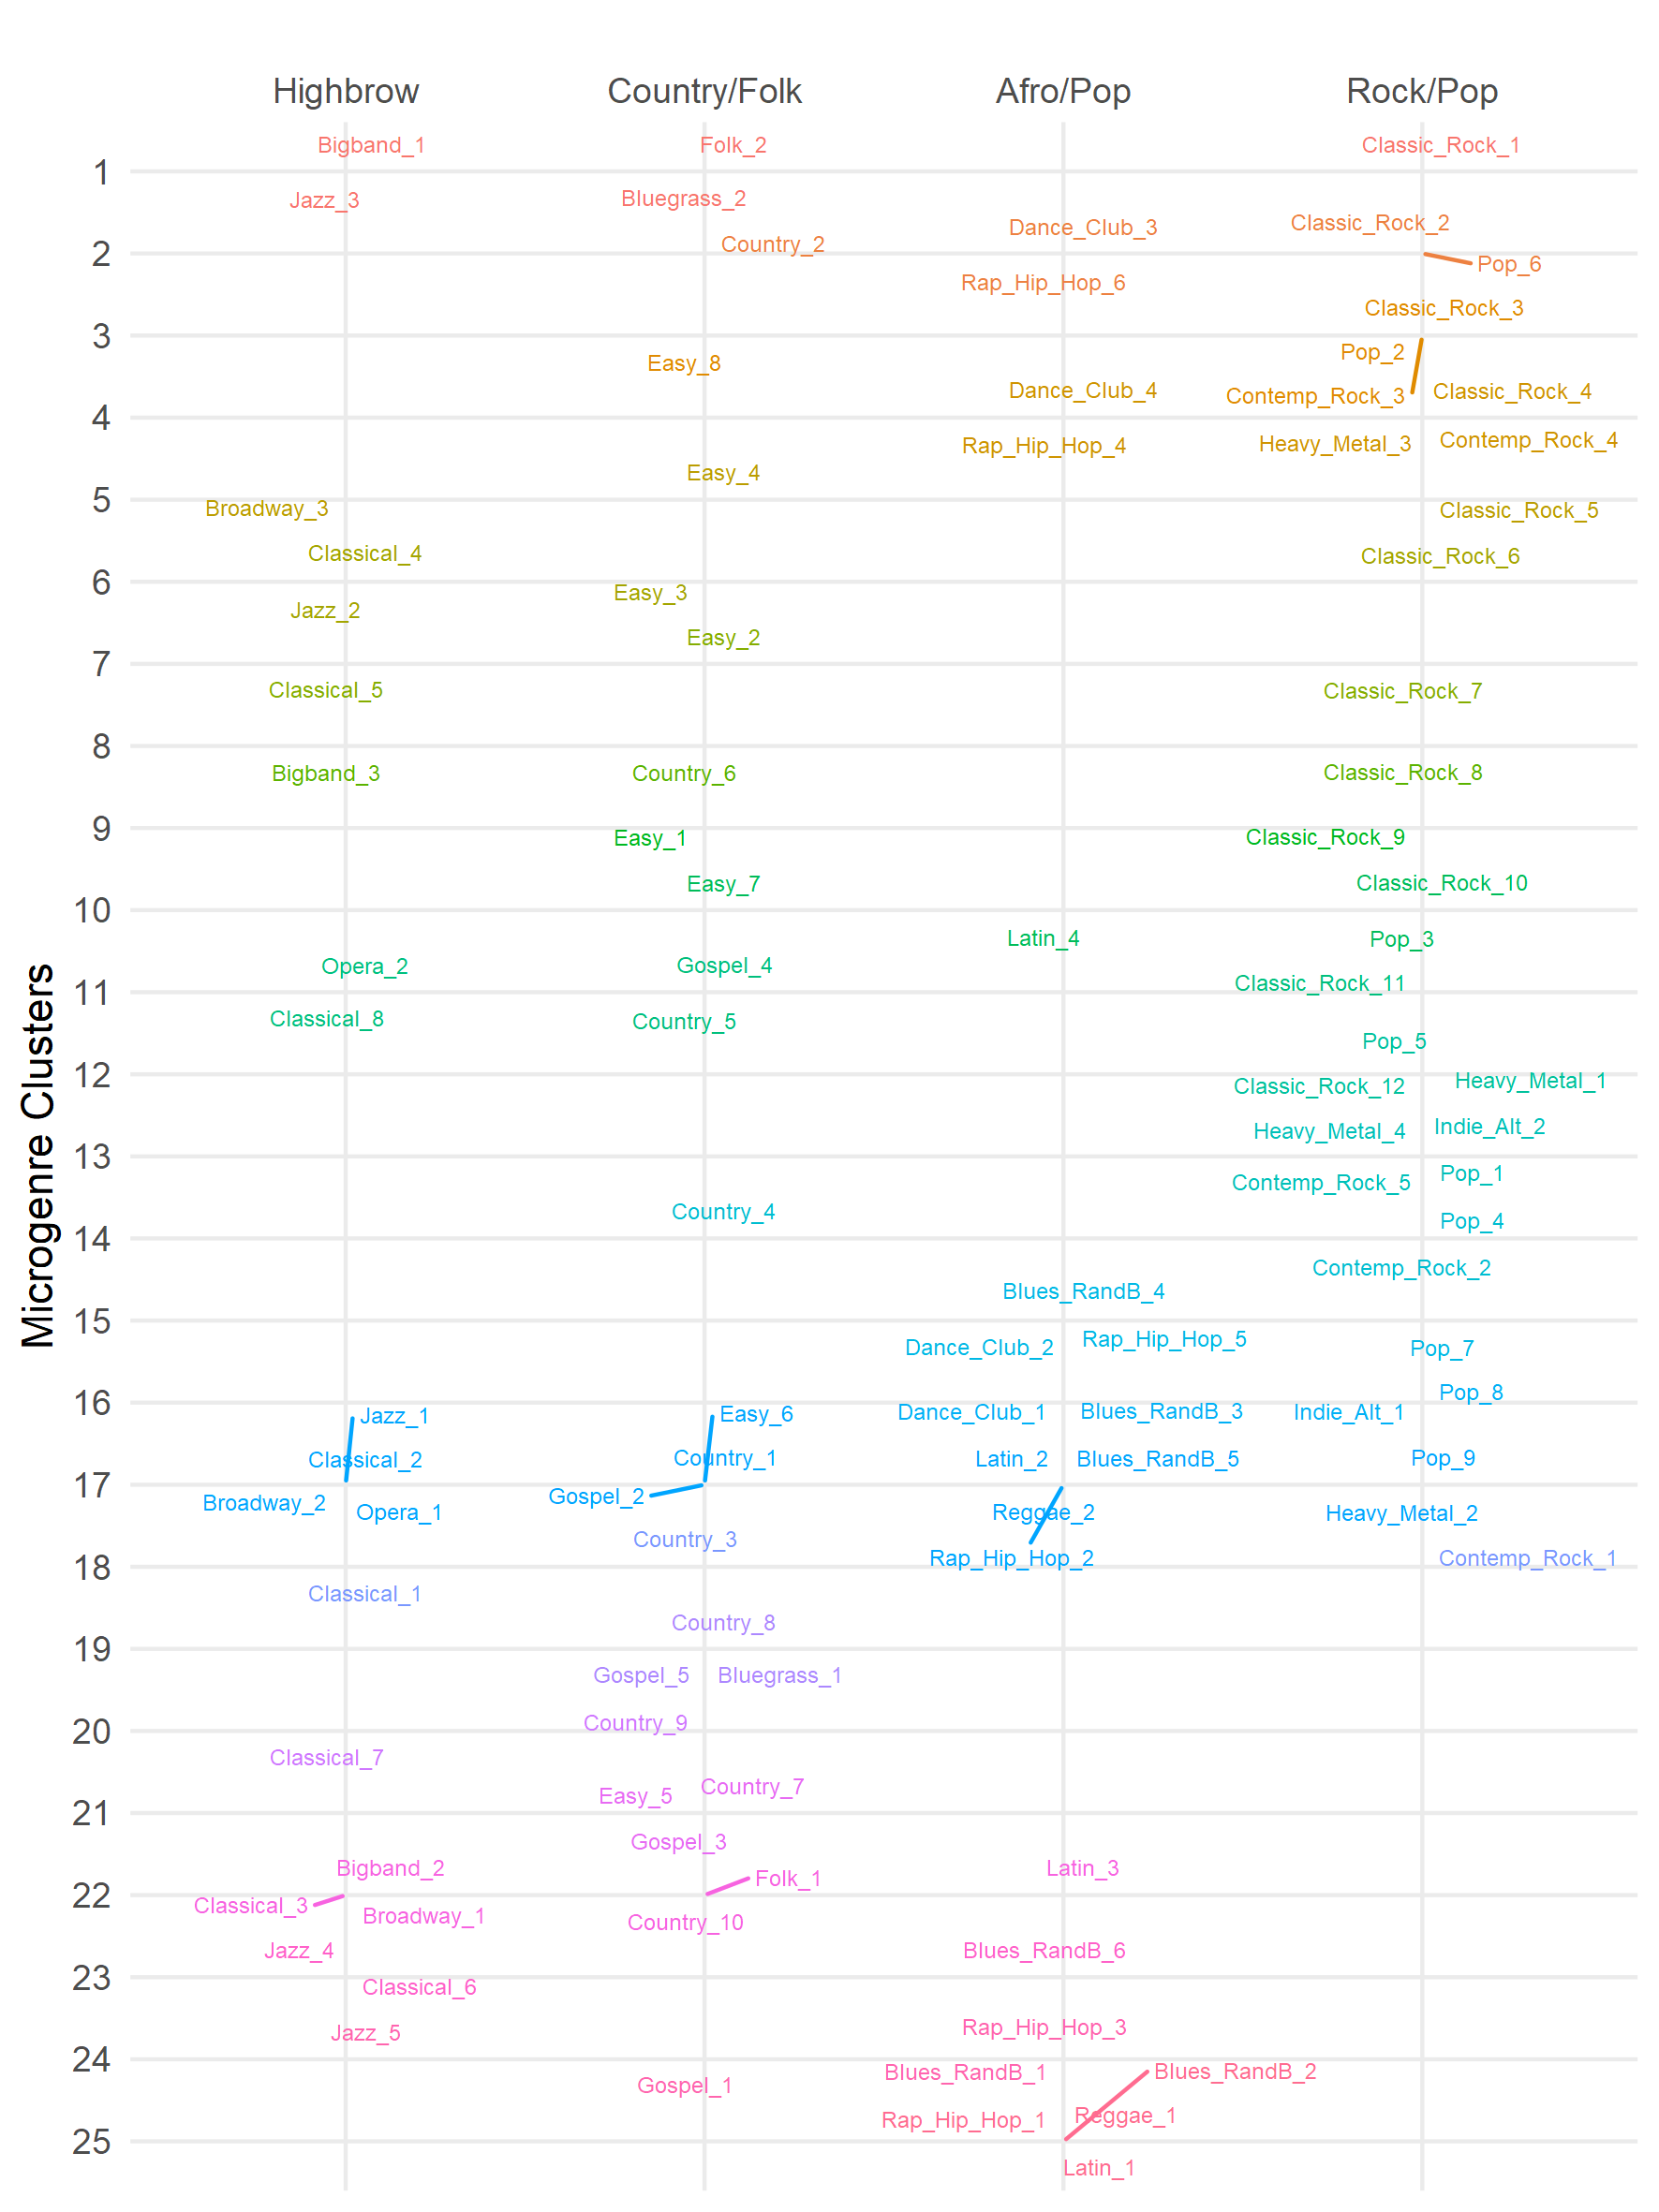
\includegraphics[width=1.0\textwidth]{Figs/Link Clust/macro-v-micro-clust.png}
    \caption{}
    \label{fig:macro-v-micro-cluster}
 \end{figure}
 
 Two contrasts are evident in the corresponding PCA-cluster plot (Figure~\ref{fig:micro-pca} for the LCD. First, the two-dimensional embedding represents the data poorly (covering less than 10\% of the variance). This makes sense since the LCD is a higher-dimensional entity, to begin with. Of more substantive importance, note that the cluster solution now presents a more complicated picture that is harder to fit into the stylized story of opposition and differentiation between broad discourses or logics. In Figure~\ref{fig:micro-pca}, micro-genres that belong to opposed or differentiated macro-discourses in Figure~\ref{fig:macro-pca} mingle freely into ``micro-discourses'' or ``micro-logics'' (e.g., combining variants of Country, Classic Rock, Classic, Gospel, and Pop) that would be harder to characterize except as varieties of ``omnivorousness.'' The problem with this approach, however, is that we will end up with more varieties of omnivorousness that we will know what to do with. 

 Figure~\ref{fig:macro-v-micro-pca} makes this point evident. In the figure, the twenty-five micro-genre clusters shown in Figure~\ref{fig:micro-pca} are plotted along the y-axis. The x-axis consists of the unordered four-category variable formed by the (labeled) clusters in Figure~\ref{fig:macro-pca}. Thus, micro-genres in the same horizontal ``row'' belong to the same micro-genre cluster; reading down the columns assigns each micro-genre to a macro-genre discourse based on their macro-genre ``parent'' label. The point of Figure~\ref{fig:macro-v-micro-pca} is evident; {\em micro-genres combine with one another in ways that typically violate the system of oppositions and differentiation posed by macro-genre discourses}. In that respect, it is clear that the way people combine micro-genres does not follow the rule book suggested by the usual dimension-reduction analyses that rely on macro-genre labels like those shown in Figure~\ref{fig:macro-pca}. Such an approach could not make sense of the micro-genre cluster combining Classical, Opera, Gospel, Country, and Classic Rock ($k_{mg}=11)$ or the set of micro-genre clusters on the bottom left of the figure combining various (presumed) ``highbrow'' and ``Folk'' micro-genres. 
 
 Of course, the standard approach cannot explain these micro-genre combination patterns. Some micro-genre clusters (e.g., $12 >=k_{mg}<=16$) stay within designated macro-genre discourse boundaries, consisting mainly of Rock/Pop and Afro/Pop combinations. Towards the top right, we see that the (very) vague macro-genre ``Classic Rock'' splits into micro-genre variants with the affinity to combine with various ``Country/Folk'' and "Highbrow'' micro-genres. The point of the micro-genre critique, however, is precisely that it is very likely that the {\em type} of Classic Rock that plays well with Rap is different, both stylistically and in terms of underlying audience, from the one that plays well with Country. In the same way, the type of Rap listened to by people who also like Classic Rock is likely to differ in consequential ways from the type of Rap listened to by people who also like to listen to Country. 

 Overall, we learn our second lesson: Audiences combine micro-genres in ways that do not respect the traditional boundaries suggested by standard data-reduction techniques applied to macro-genre labels. As such, some substantive conclusions, such as those regarding the existence of logics or discourses that explain affinities and oppositions between macro-genre categories prevalent in previous work, are likely to have been overstated and, in most cases, misleading. The principles of vision, division, and classification people use to combine and divide micro-genre categories seem to be keyed to distinctions that cut across macro-genre categories. 

 \subsubsection{Audience Segmentation and Microgenre Heterogeneity}
 A key task in the sociology of taste is linking audience engagement with particular cultural objects and genre categories to specific sociodemographic markers, primarily of class position, education, and socio-economic status, but also of such identity categories as gender, age (or generation), region of residence, and the like. This approach is crucial in getting a sense of the location of genres in social space and in making inferences about the ``status'' of genre categories themselves. 

\begin{figure}[ht!]
    \centering
    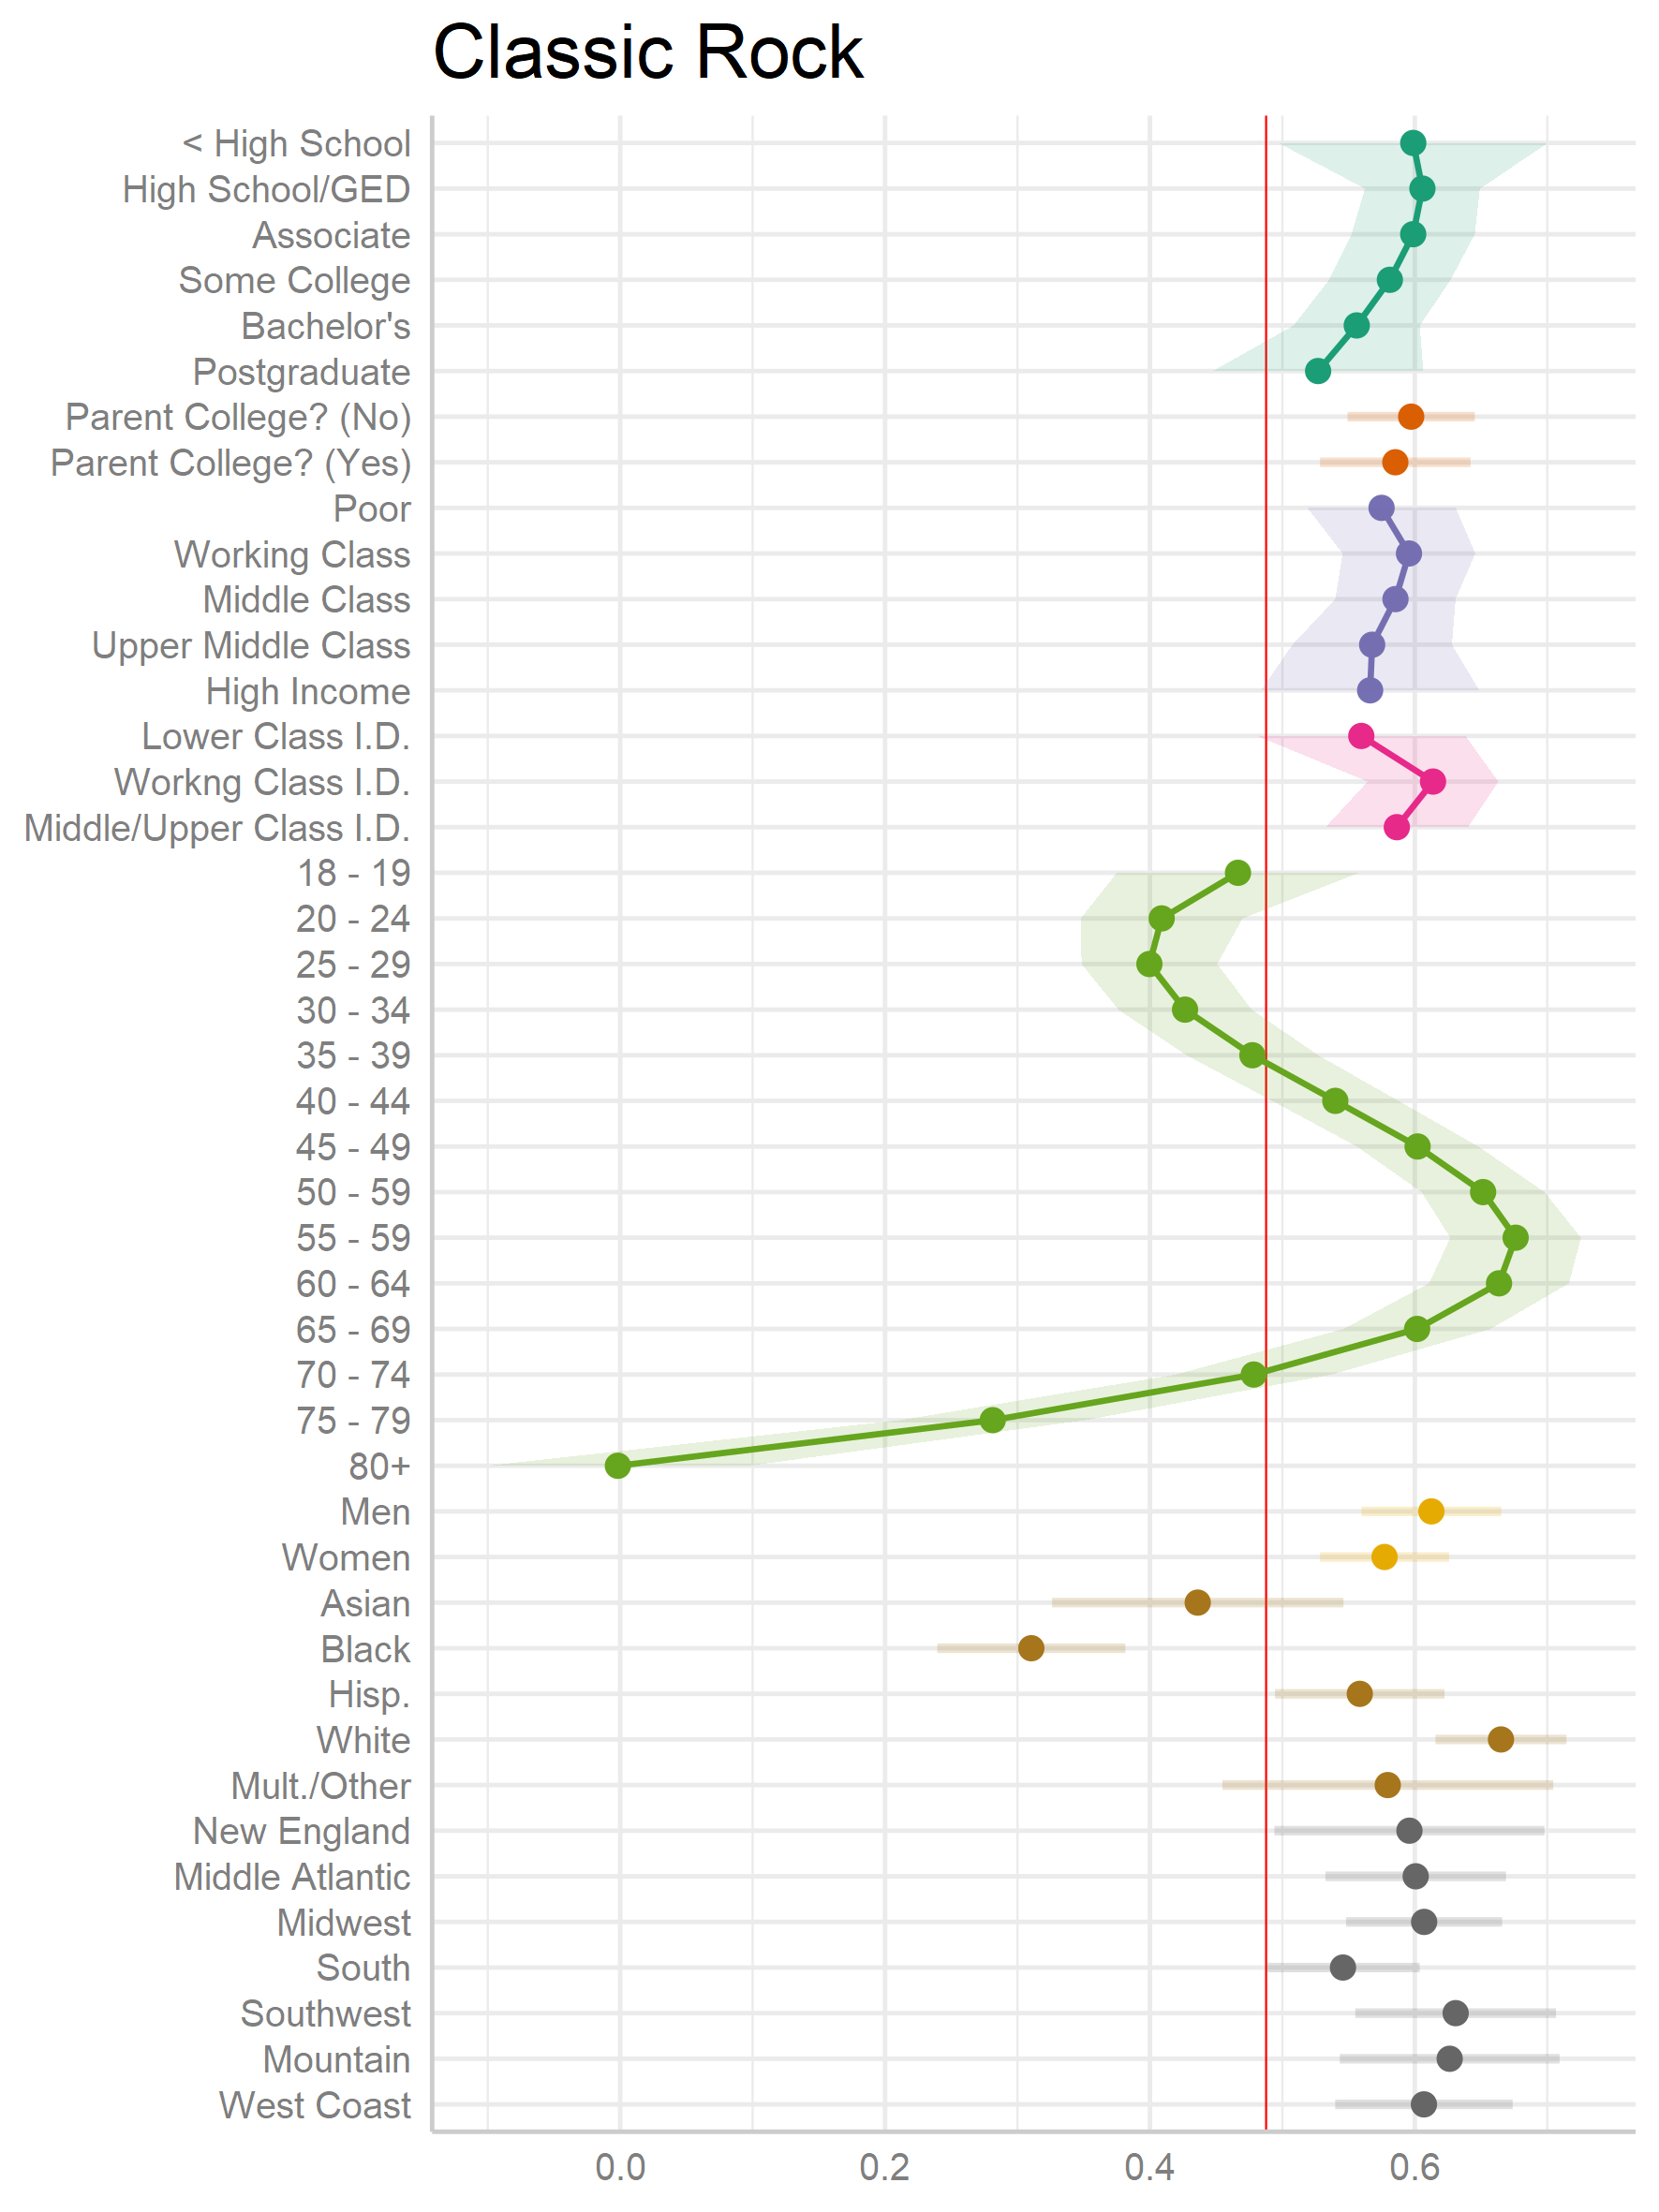
\includegraphics[width=0.8\textwidth]{Figs/Link Clust/classic-rock-macro-demog.png}
    \caption{}
    \label{fig:classic-rock-main}
\end{figure}
 
For instance, we can ascertain whether a given cluster of genres is indeed ``highbrow'' if such high-status markers of social position like higher education diplomas, high income, managerial/professional occupational status, and the like are correlated with their consumption (and the same for ``lower status'' genre categories \citep{bryson96}. The microgenre critique suggests that this crucial task will be controverted if macrogenre labels do not correspond to phenomenologically valid objects from the perspective of personal choices. That is, the conclusions that we may reach about the ``status'' of particular genre categories will be misleading if the macrogenre labels hide substantively important and relevant audience heterogeneity at the microgenre level.

\begin{figure}[ht!]
    \centering
    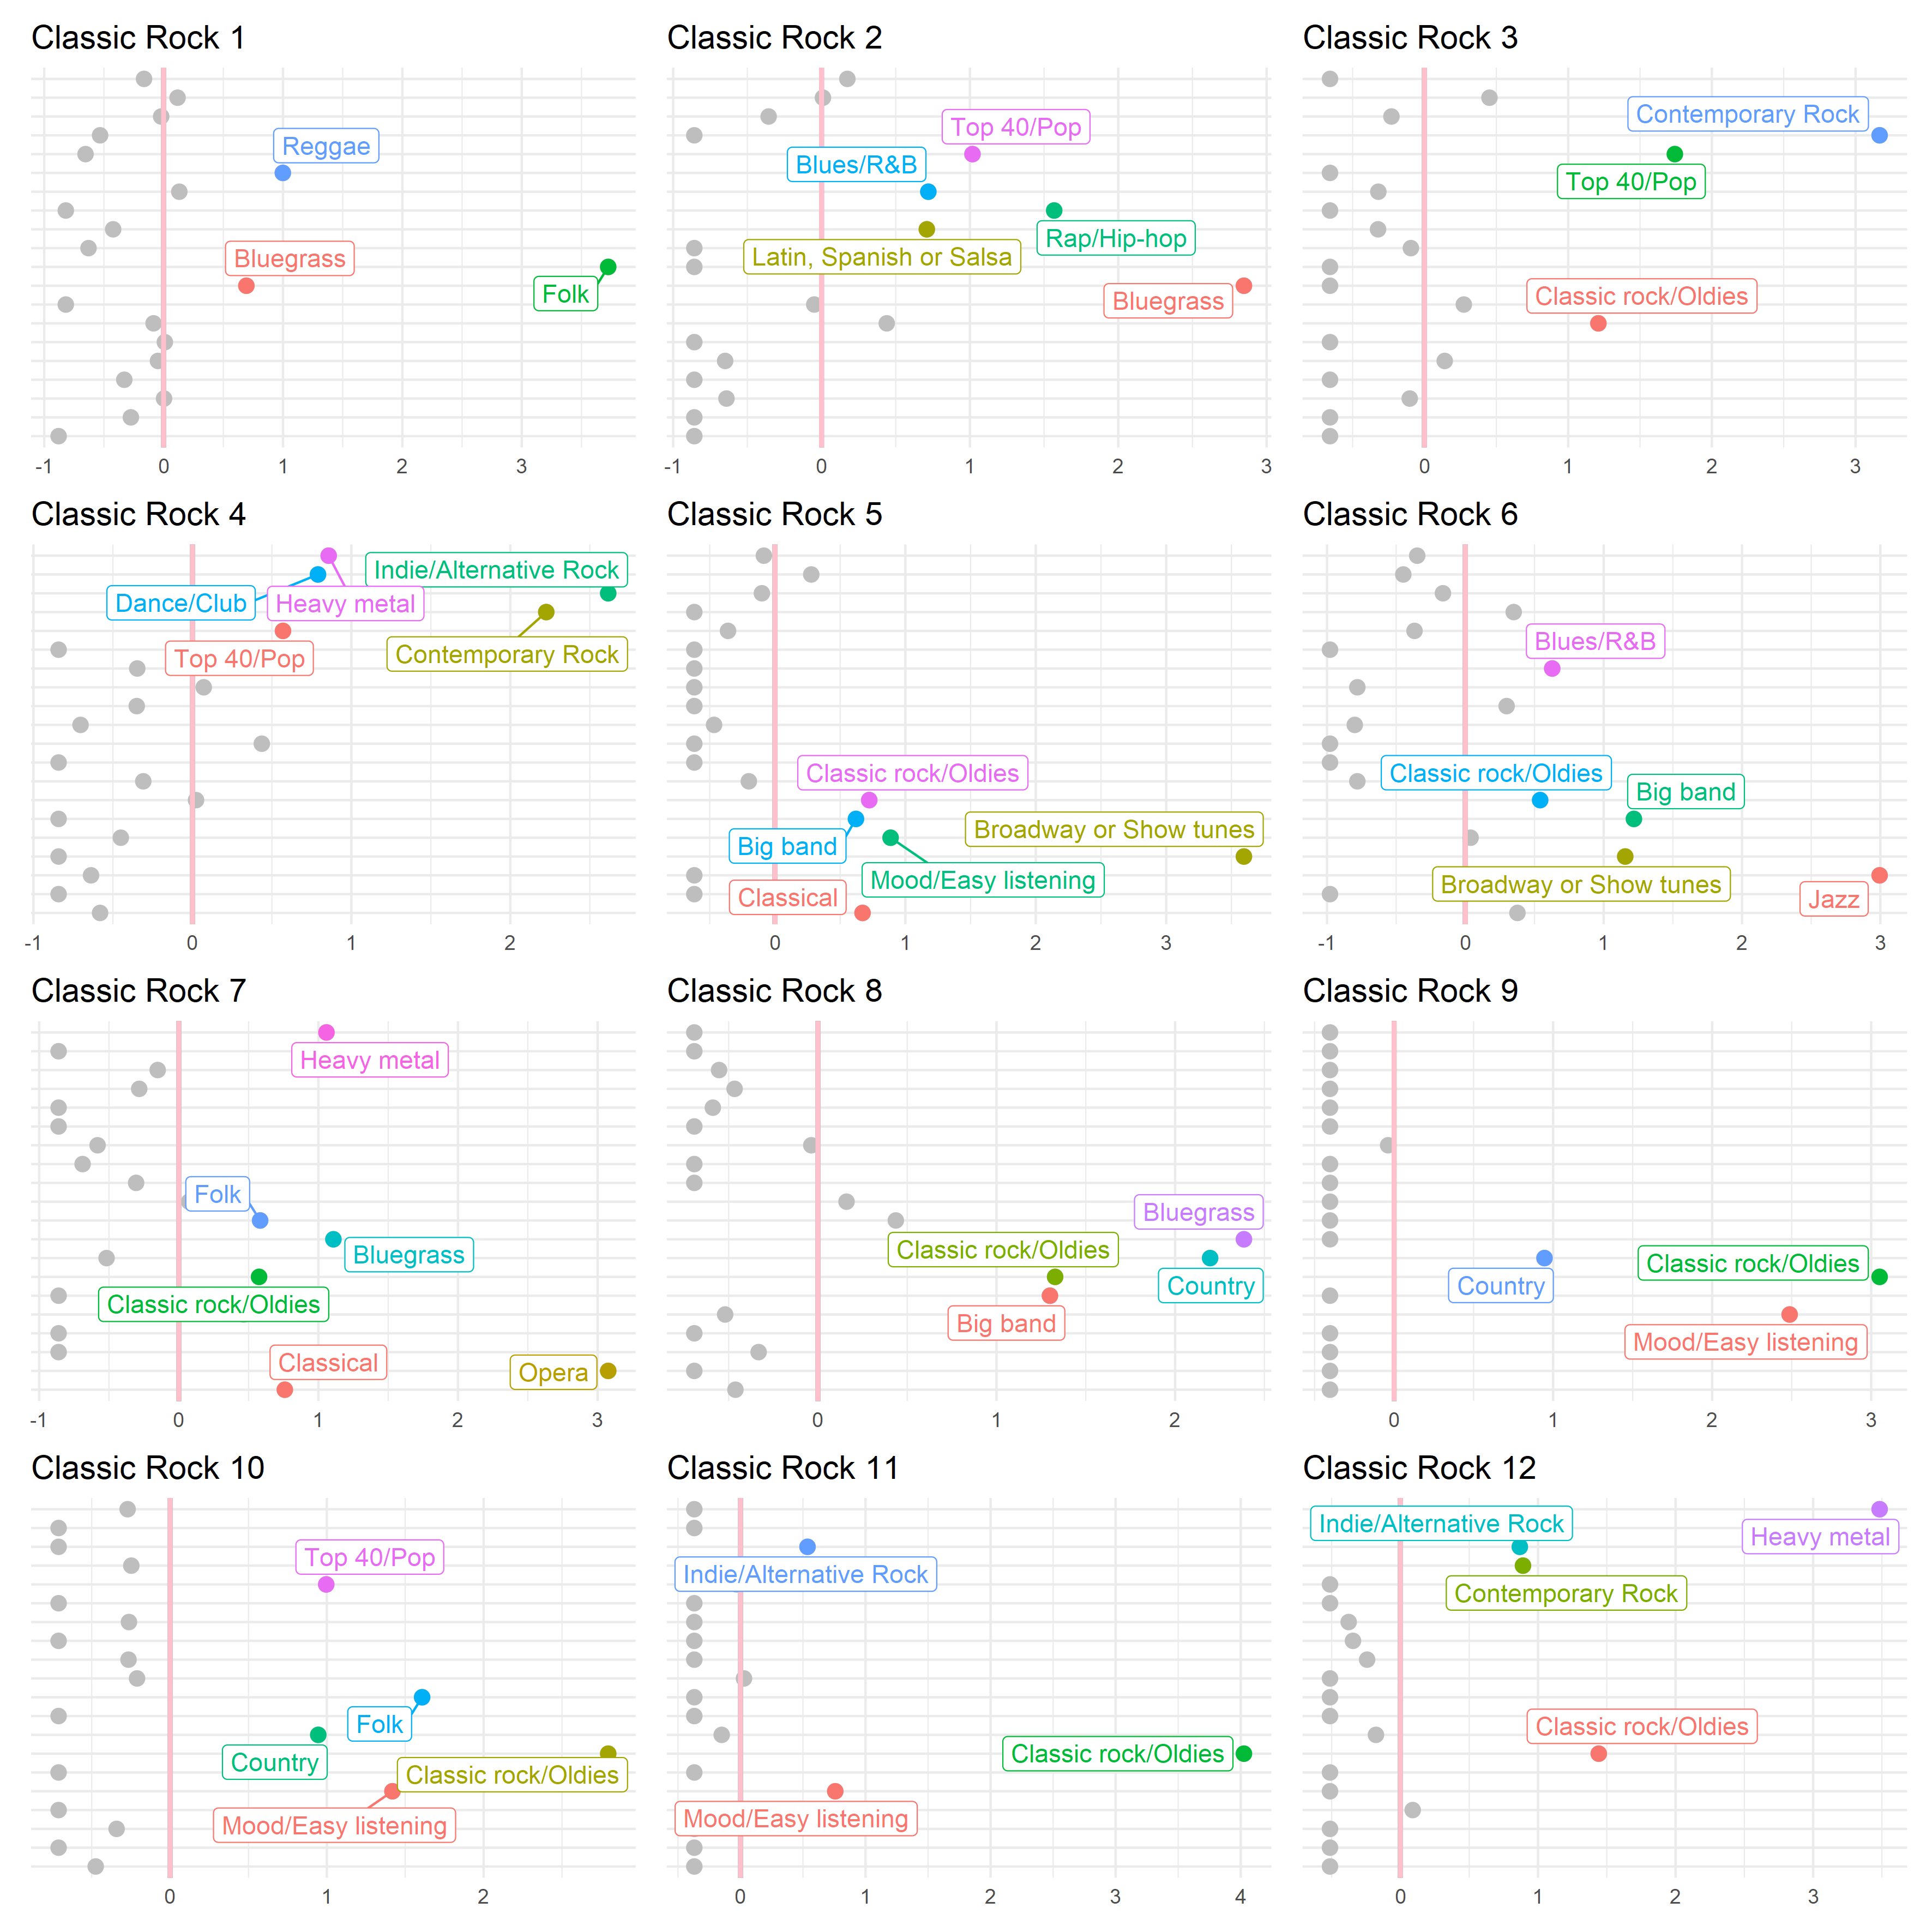
\includegraphics[width=1.0\textwidth]{Figs/Link Clust/classic-rock-fav.png}
    \caption{}
    \label{fig:fav}
\end{figure}

Let us take the case of the (very) vague (and hybrid) macrogenre label ``Classic Rock/Oldies'' as a case study (a similar exercise could be done with each of the twenty macrogenre labels). This is an instructive example since the link clustering approach divides this very broad macrogenre into the most microgenres (twelve). As shown in Figure~\ref{fig:macro-v-micro-cluster}, these micro-genres combine with most of the other micro-genres, indicative of substantial levels of stylistic diversity (and cultural meaning) within the category. If we were to follow the traditional approach, an inquiry as to the audience segmentation pattern of the vague macrogenre label ``Classic Rock,'' by, for instance, specifying a logistic regression with a binary indicator that equals one if the person reports both liking and listening to the genre and a variety of socio-demographic predictors on the right-hand side, we would end up with the results shown in Figure ~\ref{fig:classic-rock-main}. 

\begin{figure}[ht!]
    \centering
    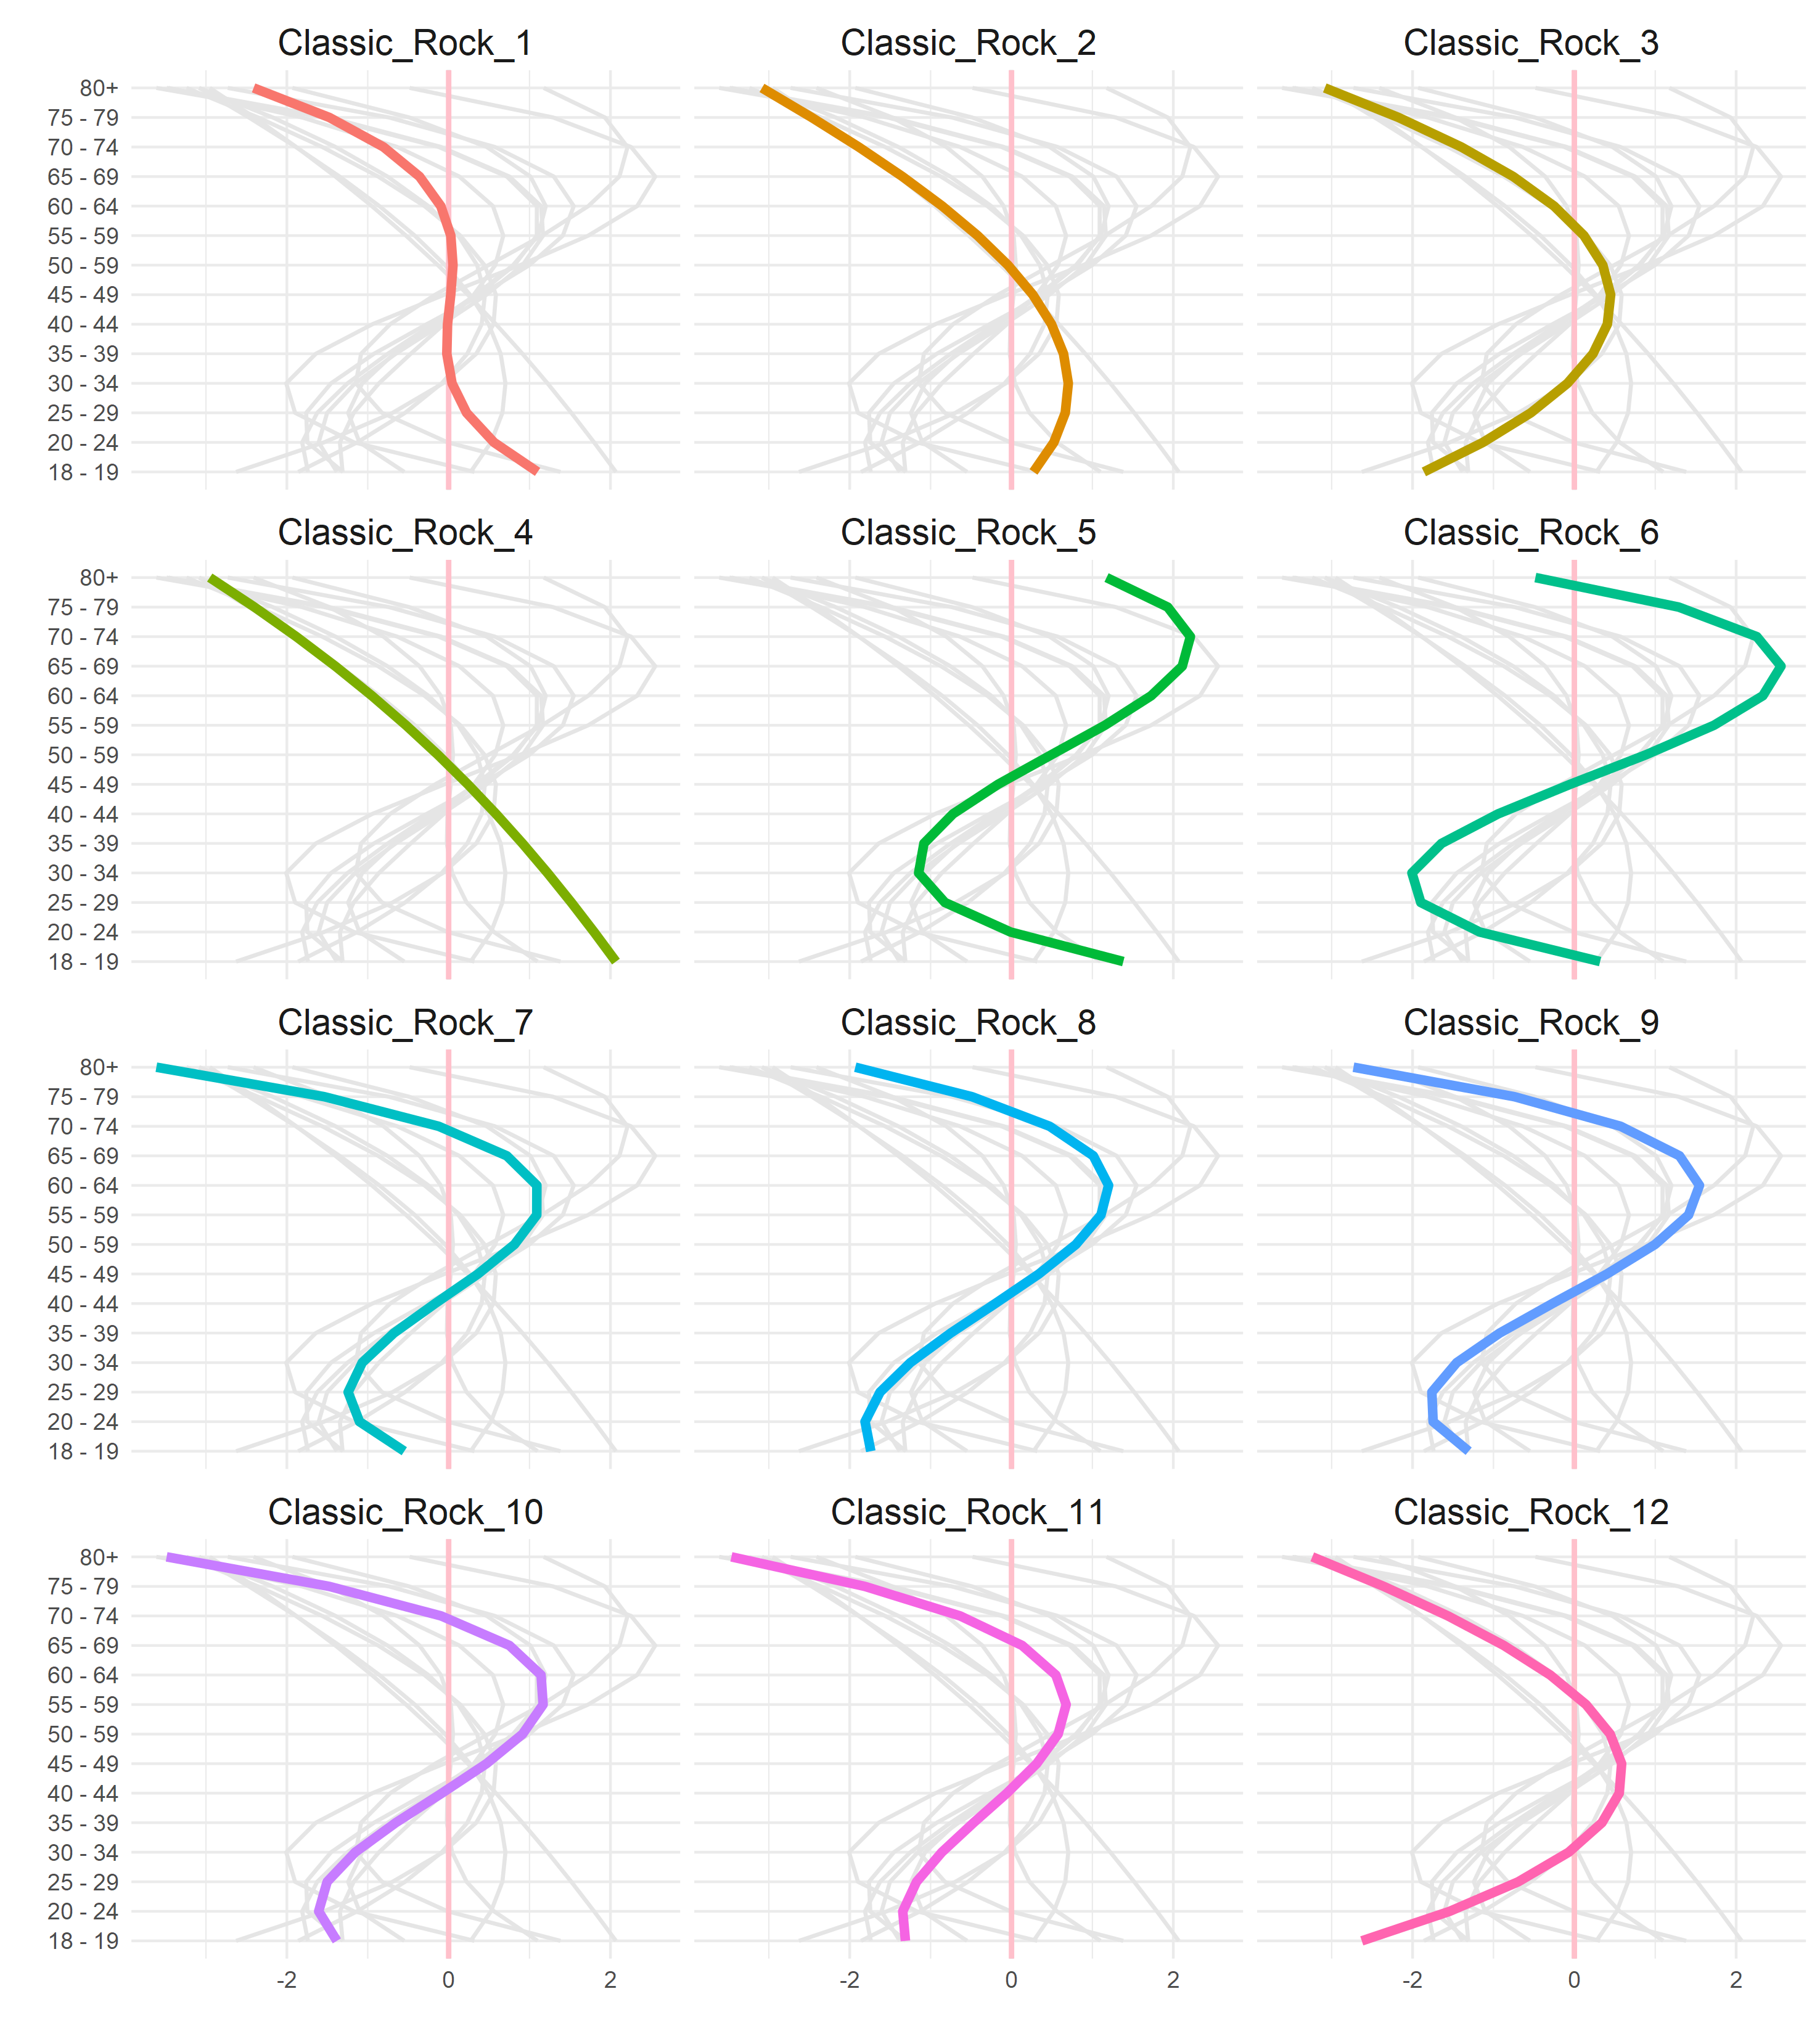
\includegraphics[width=1.0\textwidth]{Figs/Link Clust/classic-rock-age.png}
    \caption{}
    \label{fig:age}
\end{figure}
 
In the Figure, different socio-demographic characteristics are on the y-axis, and the probability of selecting the macrogenre is on the x-axis. The points represented the predicted probability, obtained from the logistic regression model that a person with that characteristic reports both listening to and liking ``Classic Rock''; the horizontal line around the point represents the 90\% confidence interval around the prediction. The red vertical line sits at the point on the x-axis, indicating the base-probability (sample average) of engaging ``Classic Rock''; points to the right of the red line indicating socio-demographic segments that are overrepresented among Classic Rock engagers, and points to the left, represent social categories underrepresented among ``Classic Rock'' engagers. 

\begin{figure}[ht!]
    \centering
    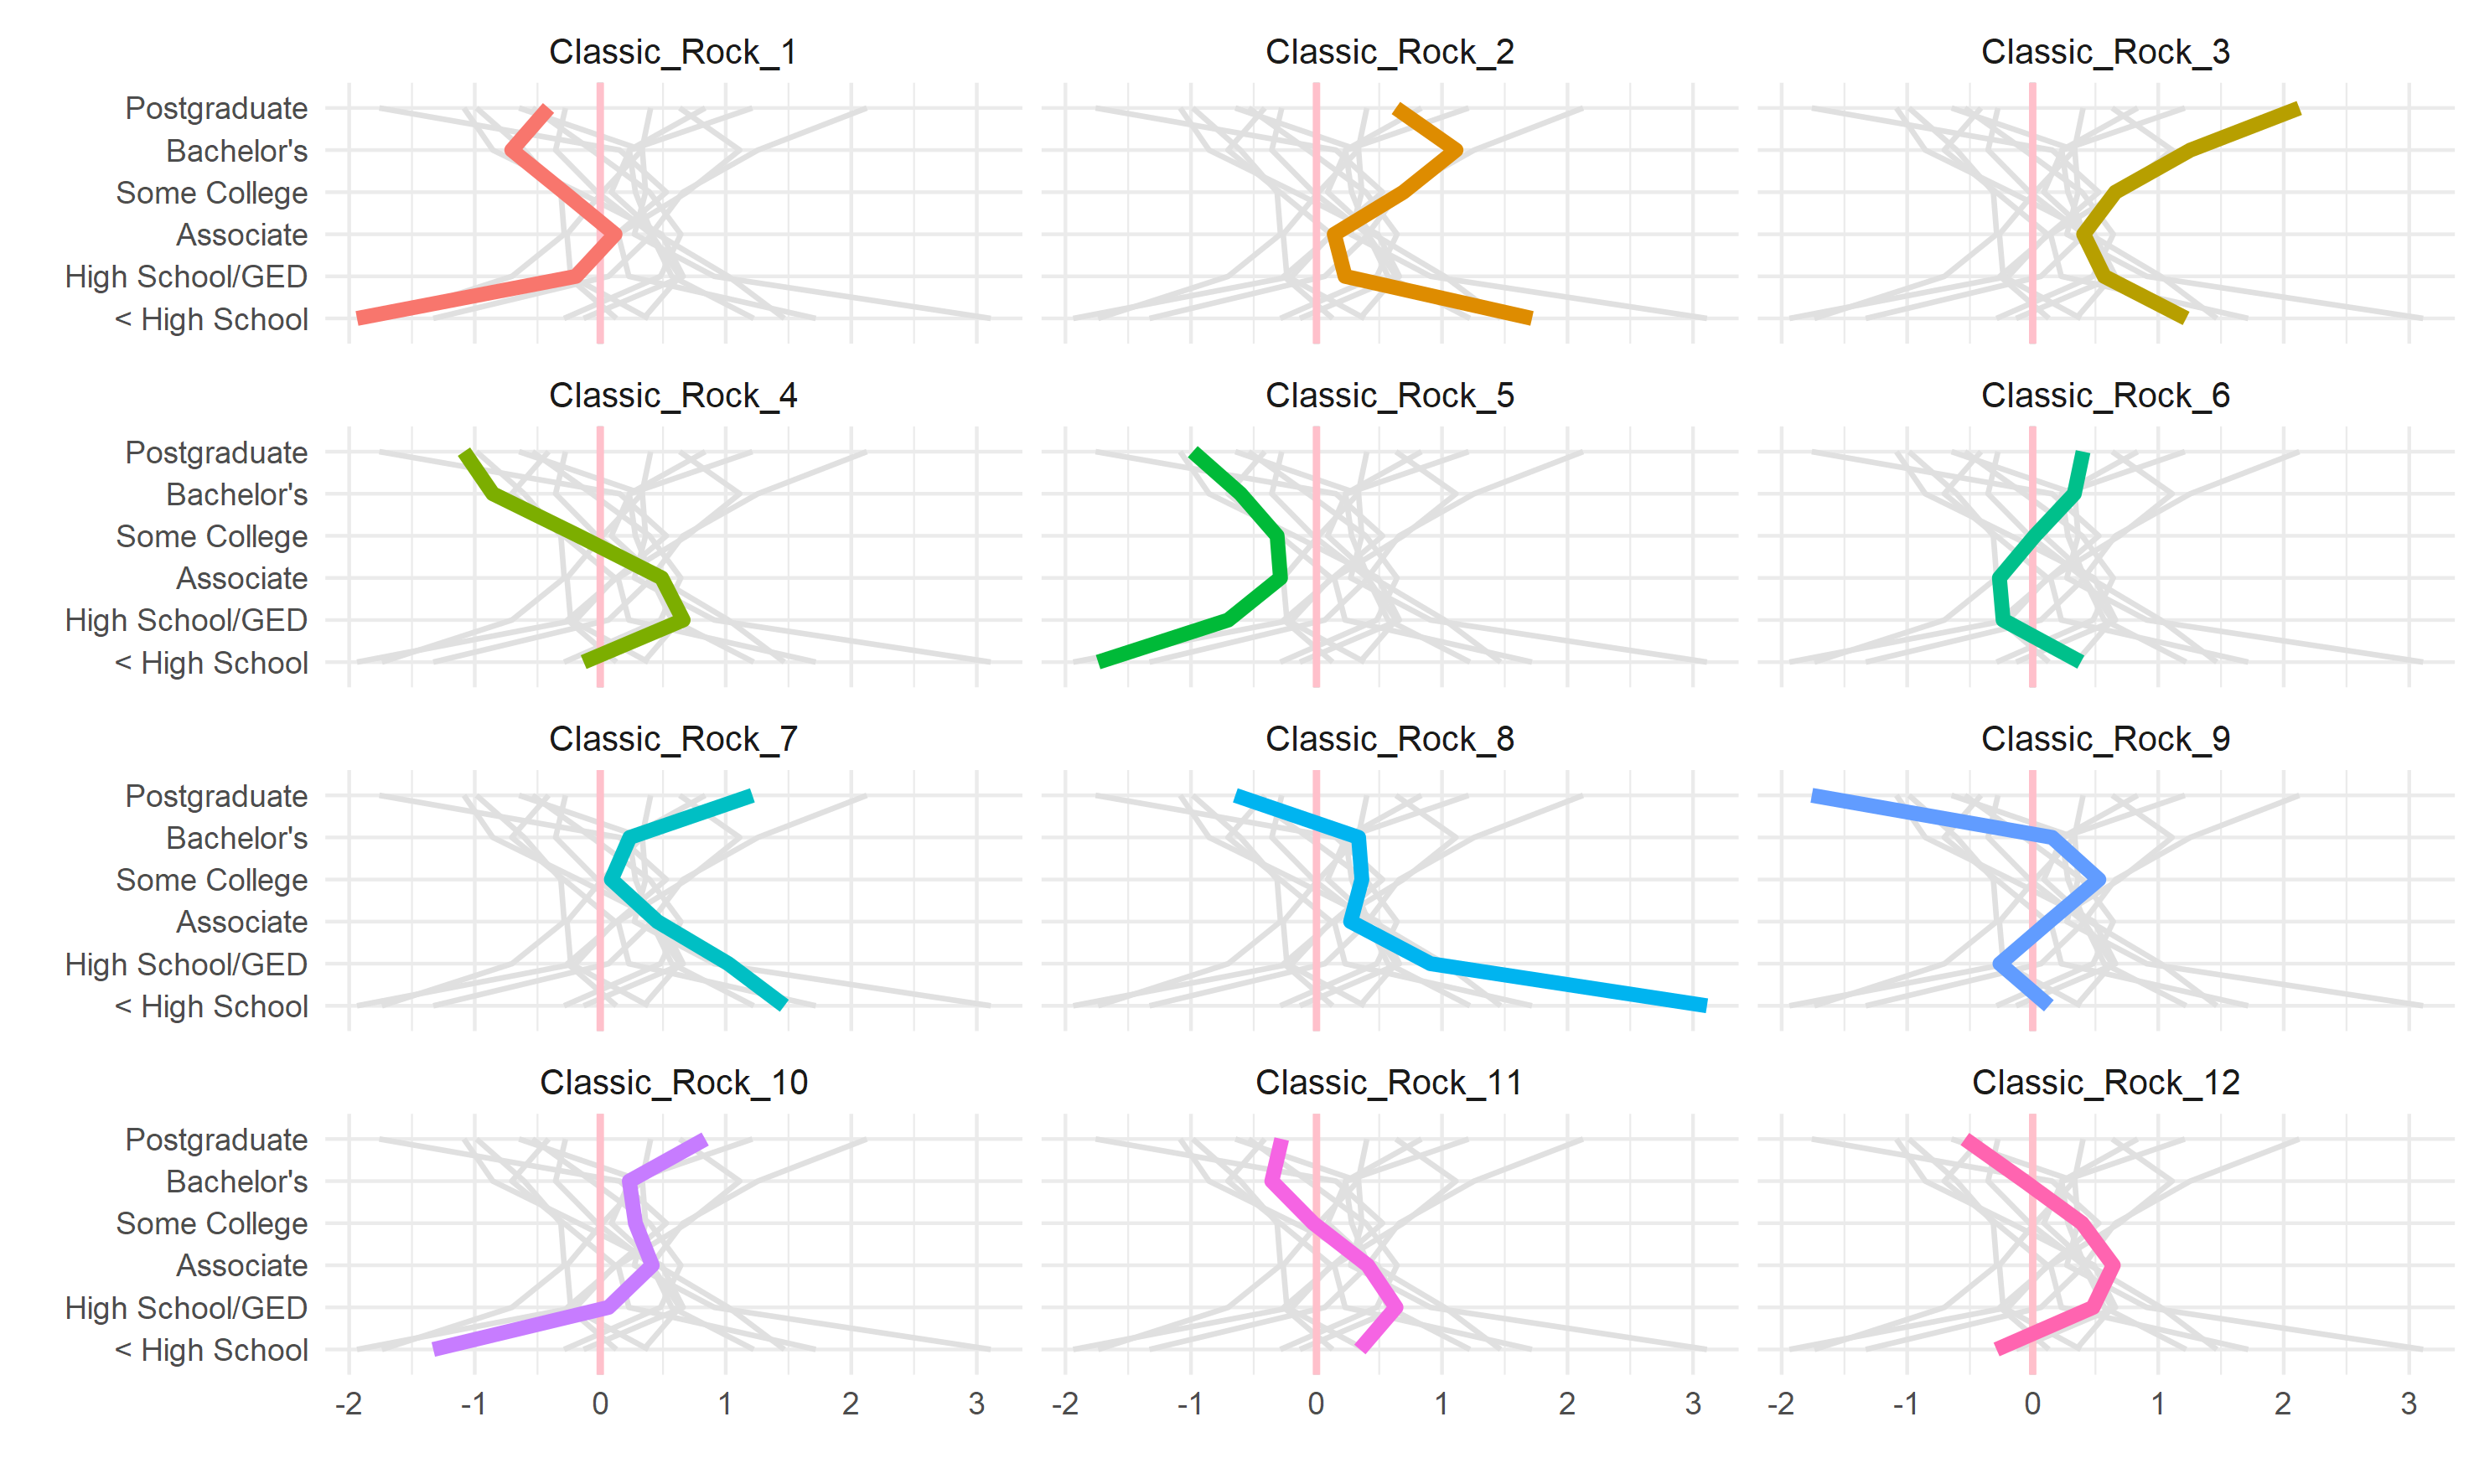
\includegraphics[width=1.0\textwidth]{Figs/Link Clust/classic-rock-educ.png}
    \caption{}
    \label{fig:educ}
\end{figure}

If we proceed in the usual fashion, we would draw various substantive conclusions regarding ``Classic Rock'' from these results. For instance, we would conclude, looking at the curvilinear---``inverted u-shape''---pattern for the effect of age, that ``Classic Rock'' is decidedly ``middle-aged'' genre, being engaged primarily by people in their 40s, 50s, and 60s--peaking for those in their late 50s---but being less likely to be engaged young adults (people younger than 40) or the old (people in their late seventies and eighties). We would also conclude that ``Classic Rock'' is a decidedly ``white'' genre, with white people being overrepresented among listeners, Black and Asian people being underrepresented, and Hispanic people being no more or less likely to engage it. We would also conclude that, beyond the higher likelihood of people without a college degree engaging ``Classic Rock," the genre does not have much class, regional, or gender differentiation (with men, women, people of class designations, and regions comparably likely to engage it). In other words, we would conclude that in the U.S. as of the early 2010s, ``Classic Rock'' is a generationally declining, raced (as white), partially classed (concerning education) musical genre that otherwise functions as a socio-demographically ``unmarked'' form of popular culture (it is the most chosen genre in the survey). 

The corresponding analysis for the twelve microgenre variations, shown in Figures~\ref{fig:age} through~\ref{fig:race} shows that pretty much every single one of these conclusions is either wrong, misleading, or both. Each figure presents the twelve ``Classic Rock'' variations in a separate panel, with the corresponding predictor categories on the y-axis and the (scaled) predicted probability on the x-axis. To facilitate comparison, the shape of the effect (for age, education, and class) for all variations is presented in light gray, and the corresponding effect for that ``Classic Rock'' microgenre is highlighted. Figures~\ref{fig:gender} and \ref{fig:race} show a dot plot using the same data visualization strategy. Additionally, to get more insight regarding the ``Classic Rock'' taste communities revealed by the microgenre analysis, Figure~\ref{fig:fav} plots the probability (on the x-axis) that people who chose each of the ``Classic Rock'' microgenres (on separate plot panels) reports choosing one of the twenty original macrogenres as their favorite. To facilitate interpretation, only macrogenres that are one-half a standard deviation above the predicted value are highlighted, indicating the strongest macrogenre preferences.

\begin{figure}[ht!]
    \centering
    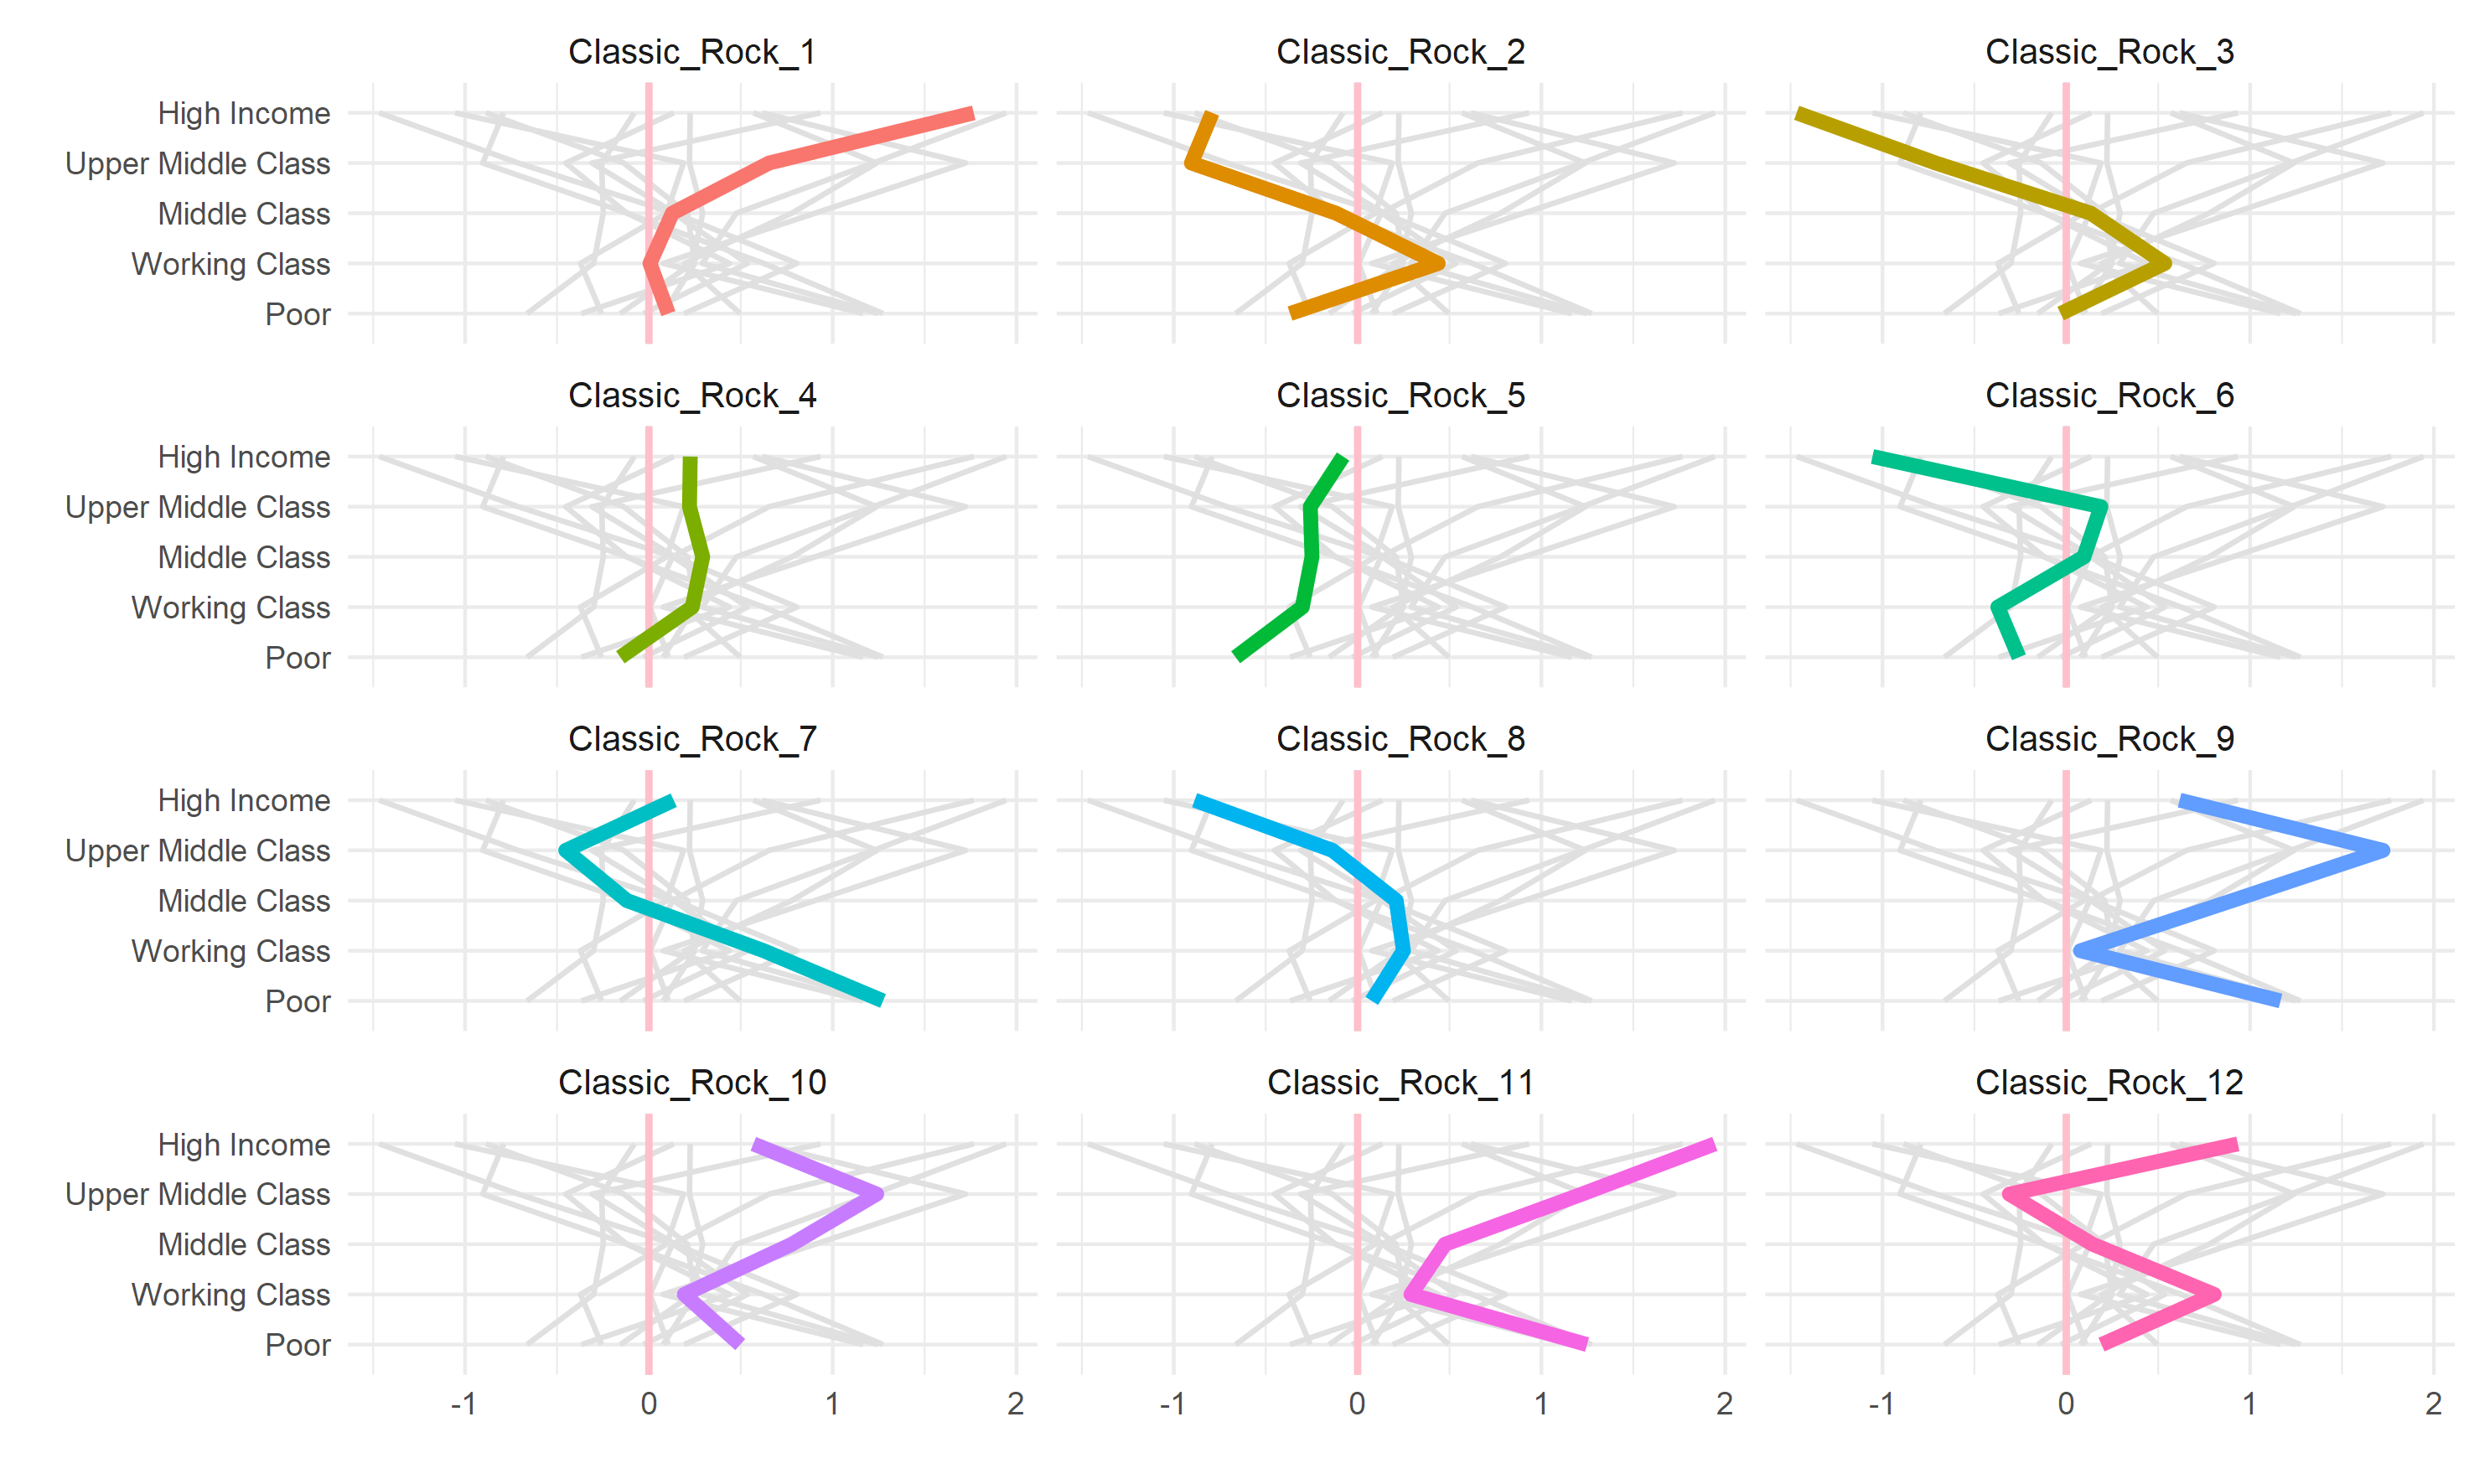
\includegraphics[width=1.0\textwidth]{Figs/Link Clust/classic-rock-class.png}
    \caption{}
    \label{fig:class}
\end{figure}
 
First, take the characterization of ``Classic Rock'' as a generationally ``middle-aged'' genre. As shown in Figure~\ref{fig:age}, the shape of the age effect varies consequentially across the different microgenre variations. As such, we could conclude that ``Classic Rock'' is relatively age-neutral (1), tilts young (2, 4), is preferred by people in their forties (3, 12), or tilts towards senior citizens (5 and 6). Even for those ``Classic Rock'' microgenres for which the peak of the inverted u-shaped effect for age is preserved for people in their fifties and sixties, the peak varies systematically. Accordingly, the characterization of ``middle-aged'' would range from people in their 50s (10, 11) or their sixties (7, 8, 9). 

\begin{figure}[ht!]
    \centering
    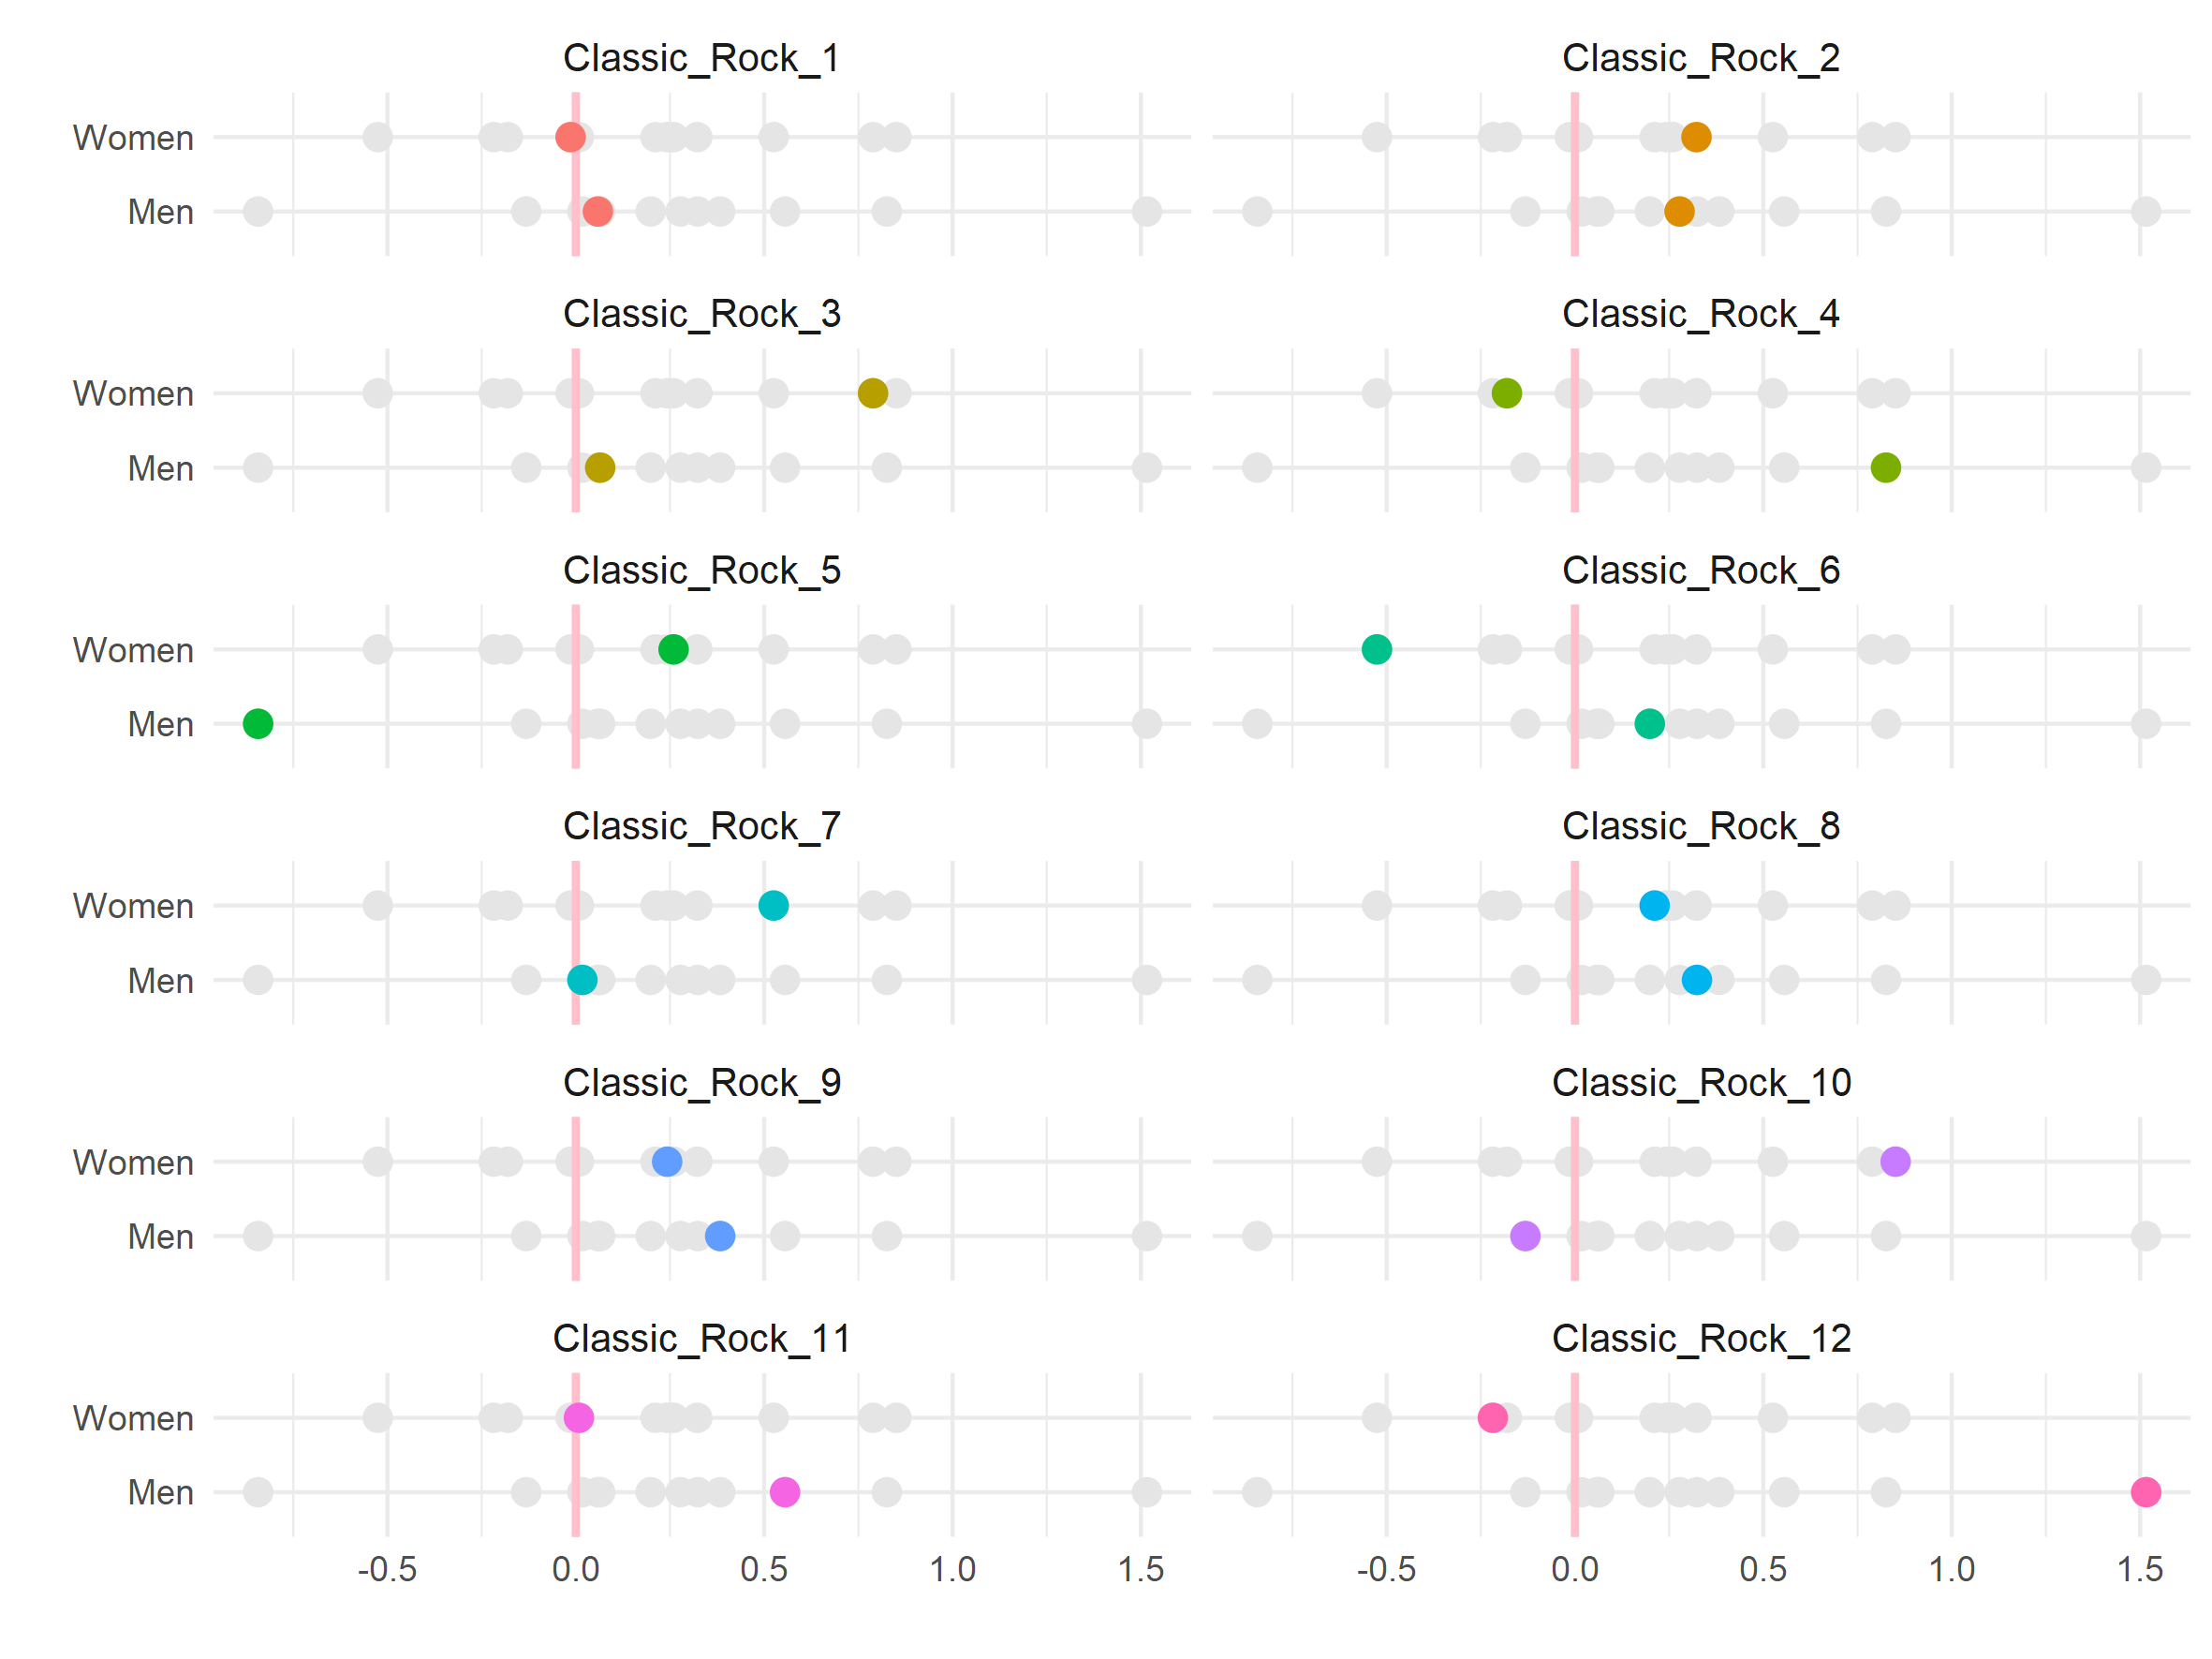
\includegraphics[width=1.0\textwidth]{Figs/Link Clust/classic-rock-gender.png}
    \caption{}
    \label{fig:gender}
\end{figure}

Looking at Figures~\ref{fig:educ} and Figure~\ref{fig:class}, we would also have to revise our conclusions about the alleged class neutrality of ``Classic Rock'' as a form of popular culture. While, indeed, some variants are class-neutral, others variants are decidedly class-inflected. For instance, (1) repels people without educational qualifications but attracts high-income people; (3) on the other hand, repels high-income people but attracts the highly educated. Variation (8) has an extreme tilt toward the less educated, and repels upper middle class and high-income people; as Figure~\ref{fig:fav} shows, fans of this Classic Rock variation are likely to report considering Bluegrass and Country as their favorite macrogenres. Other microgenre variations of ``Classic Rock'' like (10) and (11), appeal primarily to a socio-economically upper-middle class and high-income audience. Note that as shown in Figure~\ref{fig:fav} this is a variant combining preferentially with microgenre variations of Folk, Easy, and Country. These people are likely to report considering ``Classic Rock'' and Easy Listening as their favorite macrogenres. 

A similar story emerges for gender. While Figure~\ref{fig:classic-rock-main}, suggests that the macrogenre label ``Classic Rock'' is only weakly gendered, Figure~\ref{fig:gender} shows wide variation in the extent to which different microgenre variations appeal to men and women. Some like (3), (5), and (7) tilt toward women; others like (4), (11), and, particularly (12) tilt toward men. Note that fans of microgenre (12) are also disproportionately likely to report having Hard Rock/Heavy Metal as their favorite macrogenre, shedding light on its extreme tilt toward men. 

\begin{figure}[ht!]
    \centering
    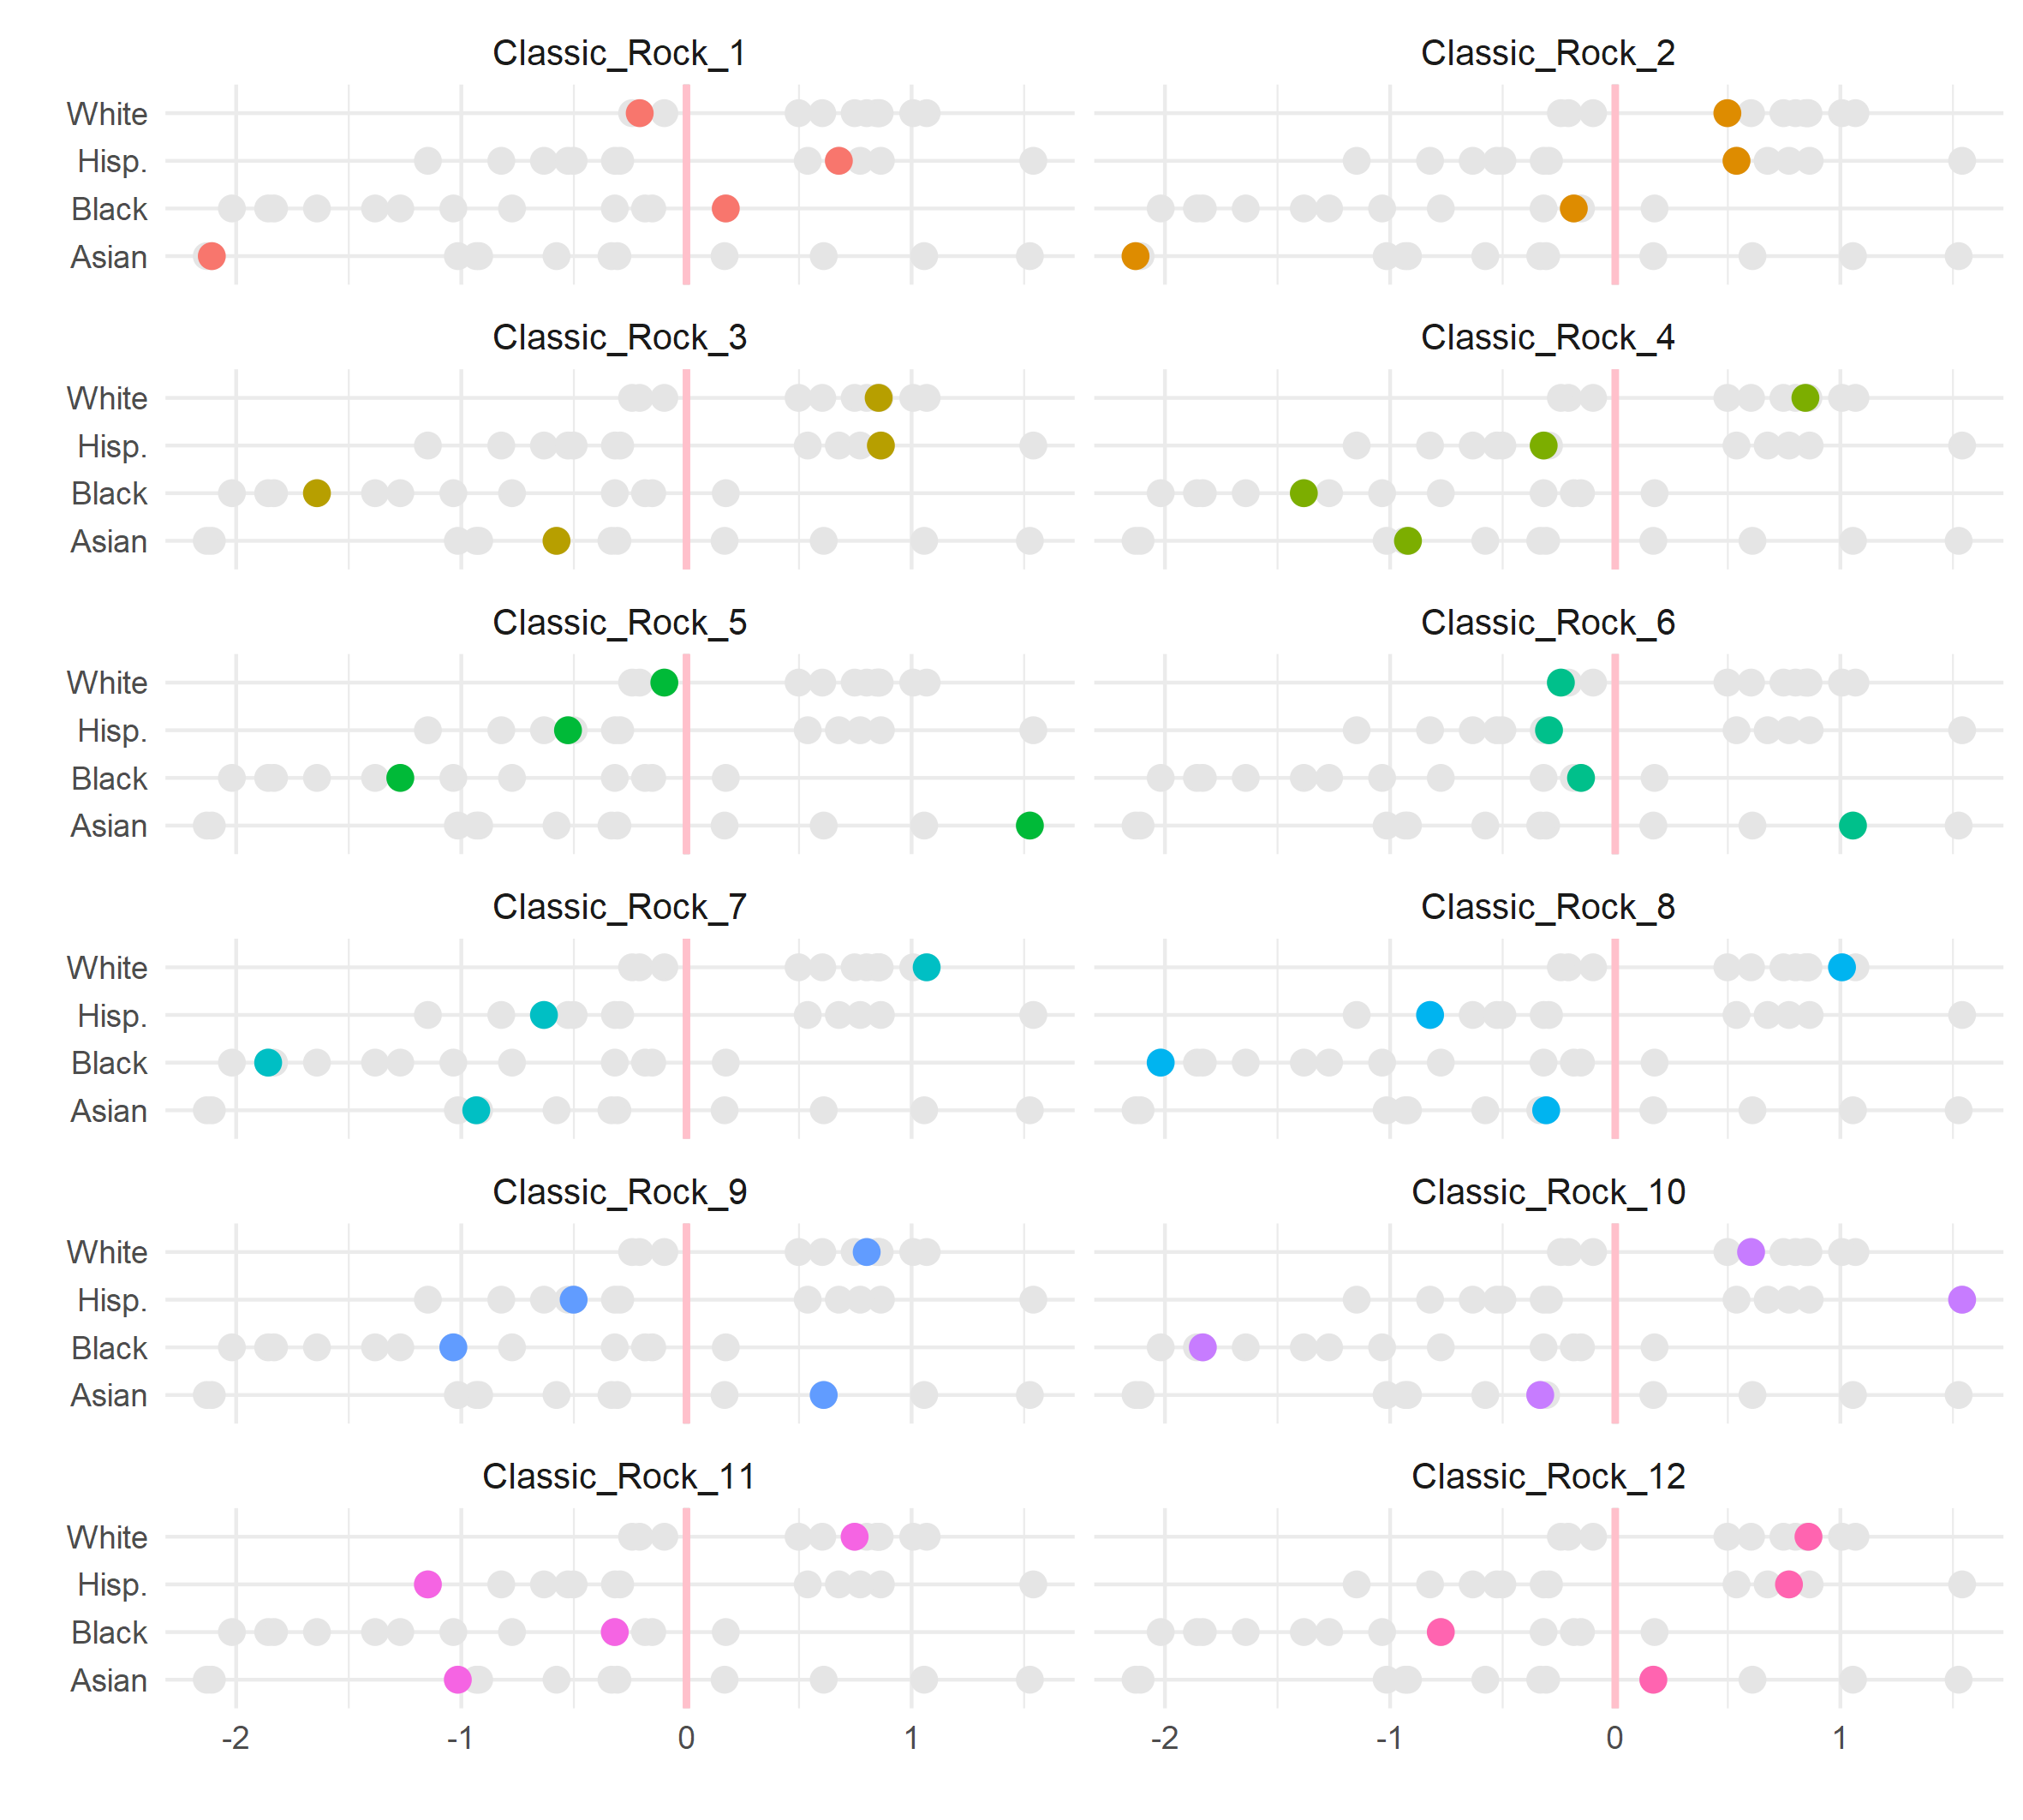
\includegraphics[width=1.0\textwidth]{Figs/Link Clust/classic-rock-race.png}
    \caption{}
    \label{fig:race}
\end{figure}

Looking at Figure~\ref{fig:race}, we can conclude that when it comes to ``Classic Rock'' having a racial tilt toward white people, the macrogenre analysis is not too misleading; most of the predicted probability estimates for this ethnoracial category are to the right of the expected mean. The same goes for its lack of appeal for people who racially identify as Black; most of the predicted probability estimates for this ethnoracial category are to the left of the expected mean for this socio-demographic category. However, the macrogenre analysis hides a lot of variation in the appeal of different variants of ``Classic Rock'' for both Hispanics and Asians. People whos self-identify as Hispanic are attracted to (1), (2), (3), and particularly (10) and (12). People who identify as Asian, on the other hand, are attracted to (5) and (6); note that as shown in Figure~\ref{fig:fav}, fans of these last two microgenre variations are also likely to report having such macrogenres as Classical, Broadway Showtunes, and Jazz as their favorites, as noted earlier these two variants also tend to have the oldest audiences. 

\section{Discussion}
Let us take stock. We began our discussion with the network or ``relational'' revolution in the quantitative study of taste in sociology \citep{pachucki2010cultural}. We noted that many good things have come from considering survey data on taste using a relational lens, including a deeper specification of core concepts in the literature and even discovering new phenomena and empirical patterns. However, we also noted that survey data are as good as the labels chosen to collect the data. A resurgent line of critics questions whether the labels that appear in our most venerable survey-based studies are true ``genres'' in the sociological (or even stylistic) sense \citep{lena2015relational, vlegels2015music}. The labels are broad, likely to be interpreted by people in heterogeneous ways, and thus hide as much as they reveal. I noted recent attempts to just drop the idea of vague macro-genre labels and either study actual sociological genres on the ground (thus partially abandoning studies of audience segmentation or at least radically reconfigure them) or ``dropping the label'' \citep{sonnett2016ambivalence} by querying people about more focused objects of taste (e.g., performers within genres). These are all important and good developments, but we also noted that they may throw away a good thing. Upping the relationality by exploiting hidden patterns in the same old vague macro-genre-based data collected before can reveal focused micro-genres. 

I proposed to do this using recent developments in the discovery of \textit{overlapping communities} in networks \citep{ahn_etal10}, which partially answers two of the challenges of macro-genre critics: The fact that actual genres are overlapping and not crisply bounded. The fact that there is hidden heterogeneity within the broad labels we usually focus on. Our analysis contrasted the application of the usual techniques to the same data, conceived in the usual ``macro" way, and \textit{after} upping the relationality and discovering the micro-genres hidden within. It is clear that focusing on micro-genres reveals variation and patterns of cultural choice (as well as audience segmentation) that we would not have noticed using the standard approach (in this, the critics are right). Still, we could do this without dropping the label or querying people about hundreds of micro-styles (most of which they'd be unfamiliar with). Instead, we exploited the venerable principle, etched into classical approaches to defining genres in network terms \citep{dimaggio1987classification}, noting that if genres are defined by the people that choose them, then they are also defined by the other choices that people make when they choose them; the country that combines with one version of Classical may not be the same country that combines with a version of the Blues (and neither is the same as the country that refuses to combine with any other style). 

The approach here is general and can be applied to studying other genre complexes beyond musical taste (allowing for economic data collection) and to studying other processes beyond taste. This includes belief, opinion, and attitude data. Essentially allows us to move from ``vague'' responses to more focused responses by exploiting the hidden patterns in the inter-response network formed when people respond to other items. Overall, we also learned a general lesson concerning our usual people or item classification techniques: To the extent that these are applied to items that themselves are ``vaguely'' defined, they will also yield even vaguer (and perhaps less than useful) macro-classifications of those items (like ``popular'' and ``high status''). The same may be said for such macro-classifications of opinions such as ``liberal'' and ``conservative,'' which, while being the primary way we interpret how people split themselves into groups by the beliefs they choose to hold, is decreasingly apt today if they ever were. 
 

\bibliography{refs.bib}
\end{document}
